\documentclass[titlepage]{report}
\usepackage[BibLaTeX,noParIndent,InlineTodonotes]{multipack}

\title{Computational Materials Science - Molecular Dynamics}
\author{Schippers, C.F.}
\date{\today}


\begin{document}
\setAbstract{}
\inserttitletoc

\listoftodos
\newpage


\chapter{Theoretical exercises}
\section{Exercise 1}
A Gaussian polymer coil with $ N $ monomers with a distance $ a $ between each other has a mean square end-to-end distance $ \left\langle R^2 \right\rangle = a^2 N $ and an approximate volume $ V \sim \left\langle R^2 \right\rangle^{\frac{3}{2}} = a^3 N^{\frac{3}{2}} $ \parencite{Rubinstein2003}. The actual volume which is occupied by the monomers with volume $ v $ of the polymer is given by $ V\sub{pol} = v N $. The volume fraction $ \phi = \frac{V\sub{pol}}{V} $ is then given by
\begin{equation}
	\phi \sim \frac{v N}{a^3 N^{\frac{3}{2}}} = \frac{v}{a^3} N^{-\frac{1}{2}}.
\end{equation}

As two-particle interactions occur when one particles is found close to another, which has probability $ phi $, one can assume that $ \nu_2 $ scales as
\begin{equation}
	\nu_2 \sim N \phi \sim N^\frac{1}{2}.
\end{equation}

Analogous, three-particle interactions occur only when two particles are found close to another particle, which has probability $ \phi^2 $, one can assume that $ \nu_3 $ scales as
\begin{equation}
	\nu_3 \sim N \phi^2 \sim N^0.
\end{equation}

As one can see $ \nu_2 $ increases with increasing $ N $ so becomes a significant contribution for a polymer, whereas $ \nu_3 $ remains small as it does not depend on $ N $.

\section{Exercise 2}
\subsection{Exercise 2a}\label{subsec:THEX2a}
The Lennard-Jones potential is given by
\begin{equation}\label{eq:LennardJones}
	U = 4 \varepsilon \left[ \left(\frac{\sigma}{r}\right)^{12} - \left(\frac{\sigma}{r}\right)^6\right].
\end{equation}

To find the minimum of this potential, take the derivative to $ r $ and put to zero for $ r = r\sub{min} $
\begin{equation}
	\left. \pd{U}{r} \right|_{r=r\sub{min}} = 4 \varepsilon \left[ -12 \frac{\sigma^{12}}{r\sub{min}^{13}} + 6\frac{\sigma^{6}}{r\sub{min}^{7}} \right] = 0.
\end{equation}

This solves to
\begin{equation}
	r\sub{min} = \sqrt[6]{2} \sigma.
\end{equation}

Putting this in $ U $ gives
\begin{equation}
	U\left(r = r\sub{min}\right) = - \varepsilon.
\end{equation}

\subsection{Exercise 2b}
$ D_e $ is the depth of the potential well. 
A Taylor expansion of the potential around $ l - l_0 = 0 $ gives
\begin{subequations}
	\begin{align}
		v(l) =& D_e \left[ 1 - \exp\left(-a (l-l_0)\right) \right]^2 \\
		\approx& a^2 D_e (l-l_0)^2 + \mathcal{O}\left((l-l_0)^3\right).
	\end{align}
\end{subequations}
So at small deviations from $ l_0 $ the Morse potential is approximately equal to a harmonic potential $ v(l) = k/2 (l-l_0)^2 $ with $ k = 2 a^2 D_e $.
At distances away from the equilibrium the Morse potential deviates from the harmonic potential as the Morse potential approaches the potential depth $ D_e $ asymptotically. 
The Morse potential and the Taylor expansion around $ l - l_0 = 0 $ are shown in \cref{fig:THEX2b}.
\begin{figure}[h!]
	\centering
	% GNUPLOT: LaTeX picture with Postscript
\begingroup
  \makeatletter
  \providecommand\color[2][]{%
    \GenericError{(gnuplot) \space\space\space\@spaces}{%
      Package color not loaded in conjunction with
      terminal option `colourtext'%
    }{See the gnuplot documentation for explanation.%
    }{Either use 'blacktext' in gnuplot or load the package
      color.sty in LaTeX.}%
    \renewcommand\color[2][]{}%
  }%
  \providecommand\includegraphics[2][]{%
    \GenericError{(gnuplot) \space\space\space\@spaces}{%
      Package graphicx or graphics not loaded%
    }{See the gnuplot documentation for explanation.%
    }{The gnuplot epslatex terminal needs graphicx.sty or graphics.sty.}%
    \renewcommand\includegraphics[2][]{}%
  }%
  \providecommand\rotatebox[2]{#2}%
  \@ifundefined{ifGPcolor}{%
    \newif\ifGPcolor
    \GPcolorfalse
  }{}%
  \@ifundefined{ifGPblacktext}{%
    \newif\ifGPblacktext
    \GPblacktexttrue
  }{}%
  % define a \g@addto@macro without @ in the name:
  \let\gplgaddtomacro\g@addto@macro
  % define empty templates for all commands taking text:
  \gdef\gplbacktext{}%
  \gdef\gplfronttext{}%
  \makeatother
  \ifGPblacktext
    % no textcolor at all
    \def\colorrgb#1{}%
    \def\colorgray#1{}%
  \else
    % gray or color?
    \ifGPcolor
      \def\colorrgb#1{\color[rgb]{#1}}%
      \def\colorgray#1{\color[gray]{#1}}%
      \expandafter\def\csname LTw\endcsname{\color{white}}%
      \expandafter\def\csname LTb\endcsname{\color{black}}%
      \expandafter\def\csname LTa\endcsname{\color{black}}%
      \expandafter\def\csname LT0\endcsname{\color[rgb]{1,0,0}}%
      \expandafter\def\csname LT1\endcsname{\color[rgb]{0,1,0}}%
      \expandafter\def\csname LT2\endcsname{\color[rgb]{0,0,1}}%
      \expandafter\def\csname LT3\endcsname{\color[rgb]{1,0,1}}%
      \expandafter\def\csname LT4\endcsname{\color[rgb]{0,1,1}}%
      \expandafter\def\csname LT5\endcsname{\color[rgb]{1,1,0}}%
      \expandafter\def\csname LT6\endcsname{\color[rgb]{0,0,0}}%
      \expandafter\def\csname LT7\endcsname{\color[rgb]{1,0.3,0}}%
      \expandafter\def\csname LT8\endcsname{\color[rgb]{0.5,0.5,0.5}}%
    \else
      % gray
      \def\colorrgb#1{\color{black}}%
      \def\colorgray#1{\color[gray]{#1}}%
      \expandafter\def\csname LTw\endcsname{\color{white}}%
      \expandafter\def\csname LTb\endcsname{\color{black}}%
      \expandafter\def\csname LTa\endcsname{\color{black}}%
      \expandafter\def\csname LT0\endcsname{\color{black}}%
      \expandafter\def\csname LT1\endcsname{\color{black}}%
      \expandafter\def\csname LT2\endcsname{\color{black}}%
      \expandafter\def\csname LT3\endcsname{\color{black}}%
      \expandafter\def\csname LT4\endcsname{\color{black}}%
      \expandafter\def\csname LT5\endcsname{\color{black}}%
      \expandafter\def\csname LT6\endcsname{\color{black}}%
      \expandafter\def\csname LT7\endcsname{\color{black}}%
      \expandafter\def\csname LT8\endcsname{\color{black}}%
    \fi
  \fi
    \setlength{\unitlength}{0.0500bp}%
    \ifx\gptboxheight\undefined%
      \newlength{\gptboxheight}%
      \newlength{\gptboxwidth}%
      \newsavebox{\gptboxtext}%
    \fi%
    \setlength{\fboxrule}{0.5pt}%
    \setlength{\fboxsep}{1pt}%
\begin{picture}(8496.00,5040.00)%
    \gplgaddtomacro\gplbacktext{%
      \csname LTb\endcsname%
      \put(814,704){\makebox(0,0)[r]{\strut{}$0$}}%
      \put(814,1383){\makebox(0,0)[r]{\strut{}$0.5$}}%
      \put(814,2061){\makebox(0,0)[r]{\strut{}$1$}}%
      \put(814,2740){\makebox(0,0)[r]{\strut{}$1.5$}}%
      \put(814,3418){\makebox(0,0)[r]{\strut{}$2$}}%
      \put(814,4097){\makebox(0,0)[r]{\strut{}$2.5$}}%
      \put(814,4775){\makebox(0,0)[r]{\strut{}$3$}}%
      \put(946,484){\makebox(0,0){\strut{}$-2$}}%
      \put(2271,484){\makebox(0,0){\strut{}$0$}}%
      \put(3596,484){\makebox(0,0){\strut{}$2$}}%
      \put(4921,484){\makebox(0,0){\strut{}$4$}}%
      \put(6246,484){\makebox(0,0){\strut{}$6$}}%
      \put(7571,484){\makebox(0,0){\strut{}$8$}}%
      \put(7703,2061){\makebox(0,0)[l]{\strut{}$D_e$}}%
    }%
    \gplgaddtomacro\gplfronttext{%
      \csname LTb\endcsname%
      \put(176,2739){\rotatebox{-270}{\makebox(0,0){\strut{}$v/D_e$}}}%
      \put(4258,154){\makebox(0,0){\strut{}$a(l-l_0)$}}%
      \csname LTb\endcsname%
      \put(6584,4602){\makebox(0,0)[r]{\strut{}Morse potential}}%
      \csname LTb\endcsname%
      \put(6584,4382){\makebox(0,0)[r]{\strut{}Linearised potential}}%
    }%
    \gplbacktext
    \put(0,0){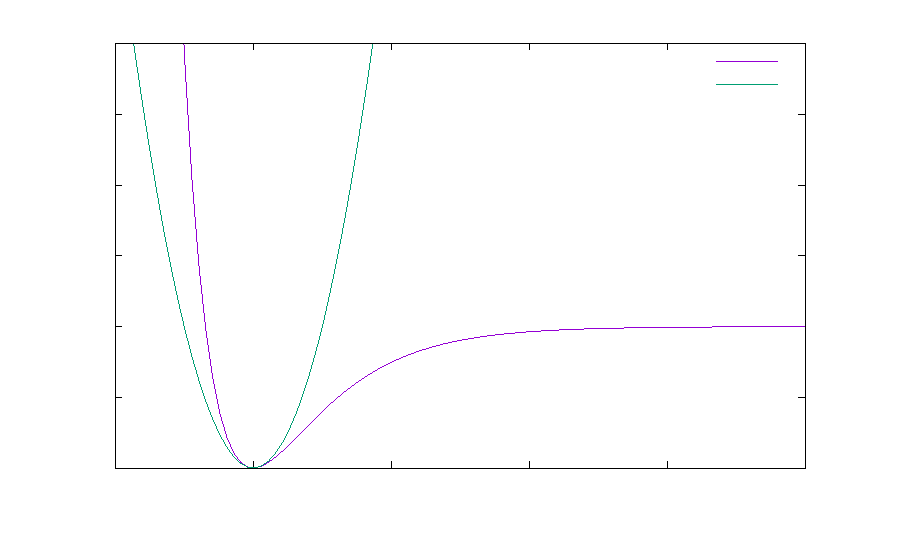
\includegraphics{THEX2b}}%
    \gplfronttext
  \end{picture}%
\endgroup

	\caption{Plot of the Morse potential and the Taylor expansion of the Morse potential around $ l-l_0 = 0 $.}
	\label{fig:THEX2b}
\end{figure}

\section{Exercise 3}
The characteristic frequency $ \omega $ of a harmonic spring with two masses is given by \cite[p. 164]{Taylor05}
\begin{equation}
	\omega = \sqrt{\frac{k\sub{spring}}{\mu}} 
\end{equation}
with $ k\sub{spring} $ the spring constant and $ \mu = \left(\frac{1}{m_1} + \frac{1}{m_2}\right)^{-1} $ the reduced mass. 
From this frequency, the wave-number $ k $ can be calculated with $ \omega = c k $, where $ c = 3\E{8}\unit{m \, s^{-1}} $ is the speed of light. This results in the values found in \cref{tab:THEX3wavenumbers}.
% Using $ 1\unit{N/m} = 1.4393 \unit{kcal \, mol^{-1} \textrm{\AA}^{-2}} $ and..
\begin{table}[h!]
	\centering
	\caption{Wave-numbers in $ \unit{cm^{-1}} $ for various bonds.}
	\label{tab:THEX3wavenumbers}
	\begin{tabular}{lr}
		Bond & Wave-number ($\unit{cm^{-1}}$) \\ 
		C-C & 4955.33 \\ 
		C=C & 7310.84 \\ 
		C=0 & 7257.00
	\end{tabular} 
\end{table}

\section{Exercise 4}
The total amount of boxes that has to be taken into account in $ N $-dimensions scales as $ C^N $.
For $ 1D $ systems this is known to be $ 3 $, for $ 2D $ systems this is $ 9 $ and for $ 3D $ systems this is $ 27 $, which leads to $ C=3 $.
So in a $ N $ dimensions the amount of periodic images is given by $ 3^N - 1 $.

\section{Exercise 5}
Using $ \vec{F} = m \ddot{\vec{r}} $, the virial $ \langle G \rangle $ can be calculated as
\begin{subequations}
	\begin{align}
		\langle G \rangle =& \left\langle \sum_i \vec{r}_i \cdot \vec{F}_i \right\rangle\\
		=& m \left\langle \sum_i \vec{r}_i \cdot \ddot{\vec{r}}_i \right\rangle.
	\end{align}
\end{subequations}

The average can be calculated using equation 2.1 from the lecture notes:
\begin{subequations}
	\begin{align}
	\langle G \rangle =& \lim\limits_{t\sub{obs} \rightarrow \infty} \frac{1}{t\sub{obs}} \int_{0}^{t\sub{obs}} m \sum_i \vec{r}_i \cdot \ddot{\vec{r}}_i \d t\\
	=& \lim\limits_{t\sub{obs} \rightarrow \infty} \frac{m}{t\sub{obs}} \left( \left. \left[\sum_i \vec{r}_i \cdot \dot{\vec{r}}_i \right] \right|_0^{t\sub{obs}} - \int_{0}^{t\sub{obs}} \sum_i \dot{\vec{r}}_i \cdot \dot{\vec{r}}_i \d t \right).
	\end{align}
\end{subequations}

As the first term vanishes as it is divided by $ t\sub{obs} $, which goes to $ \infty $. By using equation 2.1 from the lecture notes and $ \sum_i \left\langle \dot{\vec{r}}_i^{\;2} \right\rangle = N \left\langle \dot{\vec{r}}^{\;2} \right\rangle $, the remaining part can be rewritten:
\begin{subequations}
	\begin{align}
	\langle G \rangle =& - \lim\limits_{t\sub{obs} \rightarrow \infty} \frac{m}{t\sub{obs}} \int_{0}^{t\sub{obs}} \sum_i \dot{\vec{r}}_i^{\;2} \d t \\
	=& -m \left\langle \sum_i \dot{\vec{r}}_i^{\;2} \right\rangle\\
	=& -m N \left\langle \dot{\vec{r}}^{\;2} \right\rangle.
	\end{align}
\end{subequations}

As according to the equipartition theorem $ 3 k\sub{B} T = m \left\langle \vec{v}^{\;2} \right\rangle = m \left\langle \dot{\vec{r}}^{\;2} \right\rangle $, the virial is given by $ \langle G \rangle = -3 n k\sub{B} T $.\\

Moreover, the sum $ \sum_i \vec{r} \cdot \vec{F}_i\suprm{ext} $ can be calculated using $ \d \vec{F}_i\suprm{ext} = - P \d \vec{A})_i $:
\begin{subequations}
	\begin{align}
		\sum_i \vec{r} \cdot \vec{F}_i\suprm{ext} =& \sum_i \int \vec{r} \cdot \vec{F}_i\suprm{ext}\\
		=& \sum_i \int_{A_i} P \vec{r} \cdot \d\vec{A}_i.
	\end{align}
\end{subequations}

Using the Gauss theorem and the fact that $ \nabla \vec{r} = 3 $ this can be further calculated as
\begin{subequations}
	\begin{align}
		\sum_i \int_{A_i} P \vec{r} \cdot \d\vec{A}_i =& -P \sum_i \int_{V_i} \nabla \cdot \vec{r}_i \d V_i\\
		=& -3 P \sum_i V_i\\
		=& -3 P V.
	\end{align}
\end{subequations}

This results can be combined with $ \langle G \rangle = -3 n k\sub{B} T $ using $ \vec{F} = \vec{F}\suprm{int} + \vec{F}\suprm{ext} $:

\begin{subequations}
	\begin{align}
		-3 V P = \sum_i \vec{r} \cdot \vec{F}_i\suprm{ext} =& \left\langle \sum_i \vec{r}_i \cdot \vec{F}_i \right\rangle - \left\langle \sum_i \vec{r}_i \cdot \vec{F}_i\suprm{int} \right\rangle\\
		=& \langle G \rangle - \left\langle \sum_i \vec{r}_i \cdot \vec{F}_i\suprm{int} \right\rangle\\
		=& -3 N K\sub{B} T - \left\langle \sum_i \vec{r}_i \cdot \vec{F}_i\suprm{int} \right\rangle.
	\end{align}
\end{subequations}

This yields
\begin{equation}
P = \frac{1}{V} \left( N k\sub{B} T + \frac{1}{3} \left\langle \sum_i \vec{r}_i \cdot \vec{F}_i\suprm{int} \right\rangle \right).
\end{equation}

\section{Exercise 6}
\subsection{Exercise 6a}
The magnitude of the barrier separating trans and gauche isomeric states for polyethylene is $ 14 \unit{kJ / mol} $, which is equal to $ 5.65 k\sub{B} T $.

\subsection{Exercise 6b}
The Lennard-Jones time is defined as $ \tau\sub{LJ} = a\sqrt{\frac{m}{\varepsilon}} $.
For the specified model, $ a = 1 \AA $ is the size of the particle, $ m = 12 a.u. = 1.992 \E{-28} \unit{kg} $ is the mass and $ \varepsilon = 0.5 \unit{kJ / moll} = 8.3 \E{-20} \unit{J} $ is the interaction energy, so the Lennard-Jones time is given by $ \tau\sub{LJ} \approx 10^{-10} \sqrt{\frac{1.992 \E{-28}}{8.3 \E{-20}}} \approx 0.5 \unit{ps} $.
The rotational diffusion time is defined as $ \tau\sub{diff} = \frac{8 \pi \eta (l/2)^3}{k\sub{B} T} $.
With viscosity $ \eta = 1 \unit{mPa \, s} $ and temperature $ T = 300 \unit{K} $ and length $ l = 1 \AA $, this gives $ \tau\sub{diff} = \frac{8 \pi \E{-3} \E{-30}}{4.11\E{-21}} \approx 6\unit{ps} $.
An appropriate time-step would be $ \Delta t = \tau\sub{LJ} / 100 = 5 \E{-3} \unit{ps} $, as the Lennard-Jones time is the shortest time-scale. 

\section{Exercise 7}
The kinetic energy $ E\sub{k} $ and it's time derivative are given by
\begin{subequations}
	\begin{align}
		E\sub{k} =& \sum_{1=i}^{3N}\frac{1}{2} m_i v_i^2\\
		\dd{E\sub{k}}{t} =& \sum_{1=i}^{3N} m_i \dot{v}_i v_i.
	\end{align}
\end{subequations}

Using $	m_i \dot{v}_i = F_i + m_i \gamma \left(\frac{T_0}{T} -1 \right) v_i $, this can be written as
\begin{subequations}
	\begin{align}
		\dd{E\sub{k}}{t} =& \sum_{1=i}^{3N} \left( v_i F_i + m_i \gamma \left(\frac{T_0}{T} -1 \right) v_i^2 \right)\\
		=& \sum_{1=i}^{3N} v_i F_i + \gamma \left(\frac{T_0}{T} -1 \right) 2 E\sub{k}.
	\end{align}
\end{subequations}

Now using $ E\sub{k} = \frac{3}{2}N k\sub{B} T $ one can write
\begin{equation}
	\dd{E\sub{k}}{t} = \sum_{1=i}^{3N} v_i F_i + 2\gamma \left(\frac{3 N}{2} k\sub{B} T_0 - E\sub{k} \right).
\end{equation}


\chapter{Molecular Dynamics of a Simple Liquid}

\section{Exercise 1}
The model parameters are set in de main function.
The masses of the particles are determined by the variable \texttt{special}.
If $ \texttt{special} = 1 $ the particles have mass 1, but if $ \texttt{special} \neq 1 $ the particles have random masses following a Gaussian distribution centred around 1.

\section{Exercise 2}
\subsection{Exercise 2a}
The Lennard-Jones potential decreases sharply for values smaller than $ r\sub{min} = \sqrt[6]{2}\sigma \approx 1.122 \sigma $ and therefore induces a strong repulsive force, as can be seen in \cref{fig:MDSLEX2b}.
particles are initially spaced less then this $ r\sub{min} $, this force might cause particles to be displaced a multiple of the box size, which is unrealistic and thus leads to unrealistic behaviour.
Therefore, a spacing of $ r = 1.2 \sigma $ is a reasonable choice.

\subsection{Exercise 2b}
The Lennard-Jones potential is plotted in \cref{fig:MDSLEX2b}.
The minimum of the potential is $ U(r\sub{min}) = -\varepsilon $ with $ r\sub{min} = \sqrt[6]{2} \sigma $ as was calculated in theoretical exercise 2a (\cref{subsec:THEX2a}).
The asymptote for $ r \rightarrow 0 $ is $ U(r \rightarrow 0) \rightarrow \infty $ and the asymptote for $ r \rightarrow \infty $ is $ U(r \rightarrow \infty) \rightarrow 0 $.

\begin{figure}[h!]
	\centering
	%% Creator: Matplotlib, PGF backend
%%
%% To include the figure in your LaTeX document, write
%%   \input{<filename>.pgf}
%%
%% Make sure the required packages are loaded in your preamble
%%   \usepackage{pgf}
%%
%% Figures using additional raster images can only be included by \input if
%% they are in the same directory as the main LaTeX file. For loading figures
%% from other directories you can use the `import` package
%%   \usepackage{import}
%% and then include the figures with
%%   \import{<path to file>}{<filename>.pgf}
%%
%% Matplotlib used the following preamble
%%   \usepackage[utf8x]{inputenc}
%%   \usepackage[T1]{fontenc}
%%
\begingroup%
\makeatletter%
\begin{pgfpicture}%
\pgfpathrectangle{\pgfpointorigin}{\pgfqpoint{4.133858in}{2.480315in}}%
\pgfusepath{use as bounding box, clip}%
\begin{pgfscope}%
\pgfsetbuttcap%
\pgfsetmiterjoin%
\definecolor{currentfill}{rgb}{1.000000,1.000000,1.000000}%
\pgfsetfillcolor{currentfill}%
\pgfsetlinewidth{0.000000pt}%
\definecolor{currentstroke}{rgb}{1.000000,1.000000,1.000000}%
\pgfsetstrokecolor{currentstroke}%
\pgfsetdash{}{0pt}%
\pgfpathmoveto{\pgfqpoint{0.000000in}{0.000000in}}%
\pgfpathlineto{\pgfqpoint{4.133858in}{0.000000in}}%
\pgfpathlineto{\pgfqpoint{4.133858in}{2.480315in}}%
\pgfpathlineto{\pgfqpoint{0.000000in}{2.480315in}}%
\pgfpathclose%
\pgfusepath{fill}%
\end{pgfscope}%
\begin{pgfscope}%
\pgfsetbuttcap%
\pgfsetmiterjoin%
\definecolor{currentfill}{rgb}{1.000000,1.000000,1.000000}%
\pgfsetfillcolor{currentfill}%
\pgfsetlinewidth{0.000000pt}%
\definecolor{currentstroke}{rgb}{0.000000,0.000000,0.000000}%
\pgfsetstrokecolor{currentstroke}%
\pgfsetstrokeopacity{0.000000}%
\pgfsetdash{}{0pt}%
\pgfpathmoveto{\pgfqpoint{0.564740in}{0.512013in}}%
\pgfpathlineto{\pgfqpoint{3.908433in}{0.512013in}}%
\pgfpathlineto{\pgfqpoint{3.908433in}{2.281253in}}%
\pgfpathlineto{\pgfqpoint{0.564740in}{2.281253in}}%
\pgfpathclose%
\pgfusepath{fill}%
\end{pgfscope}%
\begin{pgfscope}%
\pgfpathrectangle{\pgfqpoint{0.564740in}{0.512013in}}{\pgfqpoint{3.343693in}{1.769240in}} %
\pgfusepath{clip}%
\pgfsetrectcap%
\pgfsetroundjoin%
\pgfsetlinewidth{1.003750pt}%
\definecolor{currentstroke}{rgb}{0.000000,0.000000,1.000000}%
\pgfsetstrokecolor{currentstroke}%
\pgfsetdash{}{0pt}%
\pgfpathmoveto{\pgfqpoint{1.582656in}{2.281753in}}%
\pgfpathlineto{\pgfqpoint{1.591254in}{2.059304in}}%
\pgfpathlineto{\pgfqpoint{1.602399in}{1.815961in}}%
\pgfpathlineto{\pgfqpoint{1.613545in}{1.610817in}}%
\pgfpathlineto{\pgfqpoint{1.624691in}{1.438101in}}%
\pgfpathlineto{\pgfqpoint{1.635836in}{1.292930in}}%
\pgfpathlineto{\pgfqpoint{1.646982in}{1.171169in}}%
\pgfpathlineto{\pgfqpoint{1.658127in}{1.069309in}}%
\pgfpathlineto{\pgfqpoint{1.669273in}{0.984373in}}%
\pgfpathlineto{\pgfqpoint{1.680419in}{0.913828in}}%
\pgfpathlineto{\pgfqpoint{1.691564in}{0.855523in}}%
\pgfpathlineto{\pgfqpoint{1.702710in}{0.807623in}}%
\pgfpathlineto{\pgfqpoint{1.713856in}{0.768567in}}%
\pgfpathlineto{\pgfqpoint{1.725001in}{0.737022in}}%
\pgfpathlineto{\pgfqpoint{1.736147in}{0.711853in}}%
\pgfpathlineto{\pgfqpoint{1.747293in}{0.692088in}}%
\pgfpathlineto{\pgfqpoint{1.758438in}{0.676900in}}%
\pgfpathlineto{\pgfqpoint{1.769584in}{0.665581in}}%
\pgfpathlineto{\pgfqpoint{1.780730in}{0.657524in}}%
\pgfpathlineto{\pgfqpoint{1.791875in}{0.652214in}}%
\pgfpathlineto{\pgfqpoint{1.803021in}{0.649207in}}%
\pgfpathlineto{\pgfqpoint{1.814166in}{0.648125in}}%
\pgfpathlineto{\pgfqpoint{1.825312in}{0.648646in}}%
\pgfpathlineto{\pgfqpoint{1.836458in}{0.650494in}}%
\pgfpathlineto{\pgfqpoint{1.847603in}{0.653431in}}%
\pgfpathlineto{\pgfqpoint{1.858749in}{0.657259in}}%
\pgfpathlineto{\pgfqpoint{1.869895in}{0.661804in}}%
\pgfpathlineto{\pgfqpoint{1.881040in}{0.666920in}}%
\pgfpathlineto{\pgfqpoint{1.892186in}{0.672484in}}%
\pgfpathlineto{\pgfqpoint{1.903332in}{0.678390in}}%
\pgfpathlineto{\pgfqpoint{1.914477in}{0.684548in}}%
\pgfpathlineto{\pgfqpoint{1.925623in}{0.690883in}}%
\pgfpathlineto{\pgfqpoint{1.947914in}{0.703837in}}%
\pgfpathlineto{\pgfqpoint{1.970205in}{0.716855in}}%
\pgfpathlineto{\pgfqpoint{1.981351in}{0.723299in}}%
\pgfpathlineto{\pgfqpoint{1.992497in}{0.729663in}}%
\pgfpathlineto{\pgfqpoint{2.003642in}{0.735927in}}%
\pgfpathlineto{\pgfqpoint{2.014788in}{0.742074in}}%
\pgfpathlineto{\pgfqpoint{2.025934in}{0.748091in}}%
\pgfpathlineto{\pgfqpoint{2.037079in}{0.753968in}}%
\pgfpathlineto{\pgfqpoint{2.048225in}{0.759696in}}%
\pgfpathlineto{\pgfqpoint{2.059371in}{0.765271in}}%
\pgfpathlineto{\pgfqpoint{2.070516in}{0.770687in}}%
\pgfpathlineto{\pgfqpoint{2.081662in}{0.775943in}}%
\pgfpathlineto{\pgfqpoint{2.092808in}{0.781038in}}%
\pgfpathlineto{\pgfqpoint{2.103953in}{0.785972in}}%
\pgfpathlineto{\pgfqpoint{2.115099in}{0.790745in}}%
\pgfpathlineto{\pgfqpoint{2.126245in}{0.795359in}}%
\pgfpathlineto{\pgfqpoint{2.137390in}{0.799816in}}%
\pgfpathlineto{\pgfqpoint{2.148536in}{0.804120in}}%
\pgfpathlineto{\pgfqpoint{2.159681in}{0.808272in}}%
\pgfpathlineto{\pgfqpoint{2.170827in}{0.812277in}}%
\pgfpathlineto{\pgfqpoint{2.181973in}{0.816138in}}%
\pgfpathlineto{\pgfqpoint{2.193118in}{0.819859in}}%
\pgfpathlineto{\pgfqpoint{2.204264in}{0.823443in}}%
\pgfpathlineto{\pgfqpoint{2.215410in}{0.826896in}}%
\pgfpathlineto{\pgfqpoint{2.226555in}{0.830221in}}%
\pgfpathlineto{\pgfqpoint{2.237701in}{0.833421in}}%
\pgfpathlineto{\pgfqpoint{2.248847in}{0.836502in}}%
\pgfpathlineto{\pgfqpoint{2.259992in}{0.839467in}}%
\pgfpathlineto{\pgfqpoint{2.271138in}{0.842320in}}%
\pgfpathlineto{\pgfqpoint{2.282284in}{0.845066in}}%
\pgfpathlineto{\pgfqpoint{2.293429in}{0.847707in}}%
\pgfpathlineto{\pgfqpoint{2.304575in}{0.850249in}}%
\pgfpathlineto{\pgfqpoint{2.315720in}{0.852694in}}%
\pgfpathlineto{\pgfqpoint{2.326866in}{0.855046in}}%
\pgfpathlineto{\pgfqpoint{2.338012in}{0.857309in}}%
\pgfpathlineto{\pgfqpoint{2.349157in}{0.859486in}}%
\pgfpathlineto{\pgfqpoint{2.360303in}{0.861580in}}%
\pgfpathlineto{\pgfqpoint{2.371449in}{0.863595in}}%
\pgfpathlineto{\pgfqpoint{2.382594in}{0.865534in}}%
\pgfpathlineto{\pgfqpoint{2.393740in}{0.867400in}}%
\pgfpathlineto{\pgfqpoint{2.404886in}{0.869195in}}%
\pgfpathlineto{\pgfqpoint{2.416031in}{0.870922in}}%
\pgfpathlineto{\pgfqpoint{2.427177in}{0.872585in}}%
\pgfpathlineto{\pgfqpoint{2.438323in}{0.874185in}}%
\pgfpathlineto{\pgfqpoint{2.449468in}{0.875725in}}%
\pgfpathlineto{\pgfqpoint{2.471759in}{0.878634in}}%
\pgfpathlineto{\pgfqpoint{2.494051in}{0.881332in}}%
\pgfpathlineto{\pgfqpoint{2.516342in}{0.883834in}}%
\pgfpathlineto{\pgfqpoint{2.538633in}{0.886155in}}%
\pgfpathlineto{\pgfqpoint{2.560925in}{0.888310in}}%
\pgfpathlineto{\pgfqpoint{2.583216in}{0.890312in}}%
\pgfpathlineto{\pgfqpoint{2.605507in}{0.892172in}}%
\pgfpathlineto{\pgfqpoint{2.627798in}{0.893902in}}%
\pgfpathlineto{\pgfqpoint{2.650090in}{0.895511in}}%
\pgfpathlineto{\pgfqpoint{2.672381in}{0.897009in}}%
\pgfpathlineto{\pgfqpoint{2.694672in}{0.898404in}}%
\pgfpathlineto{\pgfqpoint{2.716964in}{0.899703in}}%
\pgfpathlineto{\pgfqpoint{2.739255in}{0.900915in}}%
\pgfpathlineto{\pgfqpoint{2.761546in}{0.902046in}}%
\pgfpathlineto{\pgfqpoint{2.794983in}{0.903603in}}%
\pgfpathlineto{\pgfqpoint{2.828420in}{0.905008in}}%
\pgfpathlineto{\pgfqpoint{2.861857in}{0.906279in}}%
\pgfpathlineto{\pgfqpoint{2.895294in}{0.907429in}}%
\pgfpathlineto{\pgfqpoint{2.928731in}{0.908472in}}%
\pgfpathlineto{\pgfqpoint{2.962168in}{0.909418in}}%
\pgfpathlineto{\pgfqpoint{3.006750in}{0.910546in}}%
\pgfpathlineto{\pgfqpoint{3.051333in}{0.911541in}}%
\pgfpathlineto{\pgfqpoint{3.095915in}{0.912421in}}%
\pgfpathlineto{\pgfqpoint{3.140498in}{0.913199in}}%
\pgfpathlineto{\pgfqpoint{3.196226in}{0.914050in}}%
\pgfpathlineto{\pgfqpoint{3.251954in}{0.914784in}}%
\pgfpathlineto{\pgfqpoint{3.318828in}{0.915537in}}%
\pgfpathlineto{\pgfqpoint{3.385702in}{0.916173in}}%
\pgfpathlineto{\pgfqpoint{3.463722in}{0.916794in}}%
\pgfpathlineto{\pgfqpoint{3.552887in}{0.917375in}}%
\pgfpathlineto{\pgfqpoint{3.653198in}{0.917900in}}%
\pgfpathlineto{\pgfqpoint{3.764654in}{0.918359in}}%
\pgfpathlineto{\pgfqpoint{3.887256in}{0.918750in}}%
\pgfpathlineto{\pgfqpoint{3.898402in}{0.918781in}}%
\pgfpathlineto{\pgfqpoint{3.898402in}{0.918781in}}%
\pgfusepath{stroke}%
\end{pgfscope}%
\begin{pgfscope}%
\pgfsetrectcap%
\pgfsetmiterjoin%
\pgfsetlinewidth{1.003750pt}%
\definecolor{currentstroke}{rgb}{0.000000,0.000000,0.000000}%
\pgfsetstrokecolor{currentstroke}%
\pgfsetdash{}{0pt}%
\pgfpathmoveto{\pgfqpoint{0.564740in}{2.281253in}}%
\pgfpathlineto{\pgfqpoint{3.908433in}{2.281253in}}%
\pgfusepath{stroke}%
\end{pgfscope}%
\begin{pgfscope}%
\pgfsetrectcap%
\pgfsetmiterjoin%
\pgfsetlinewidth{1.003750pt}%
\definecolor{currentstroke}{rgb}{0.000000,0.000000,0.000000}%
\pgfsetstrokecolor{currentstroke}%
\pgfsetdash{}{0pt}%
\pgfpathmoveto{\pgfqpoint{0.564740in}{0.512013in}}%
\pgfpathlineto{\pgfqpoint{3.908433in}{0.512013in}}%
\pgfusepath{stroke}%
\end{pgfscope}%
\begin{pgfscope}%
\pgfsetrectcap%
\pgfsetmiterjoin%
\pgfsetlinewidth{1.003750pt}%
\definecolor{currentstroke}{rgb}{0.000000,0.000000,0.000000}%
\pgfsetstrokecolor{currentstroke}%
\pgfsetdash{}{0pt}%
\pgfpathmoveto{\pgfqpoint{3.908433in}{0.512013in}}%
\pgfpathlineto{\pgfqpoint{3.908433in}{2.281253in}}%
\pgfusepath{stroke}%
\end{pgfscope}%
\begin{pgfscope}%
\pgfsetrectcap%
\pgfsetmiterjoin%
\pgfsetlinewidth{1.003750pt}%
\definecolor{currentstroke}{rgb}{0.000000,0.000000,0.000000}%
\pgfsetstrokecolor{currentstroke}%
\pgfsetdash{}{0pt}%
\pgfpathmoveto{\pgfqpoint{0.564740in}{0.512013in}}%
\pgfpathlineto{\pgfqpoint{0.564740in}{2.281253in}}%
\pgfusepath{stroke}%
\end{pgfscope}%
\begin{pgfscope}%
\pgfsetbuttcap%
\pgfsetroundjoin%
\definecolor{currentfill}{rgb}{0.000000,0.000000,0.000000}%
\pgfsetfillcolor{currentfill}%
\pgfsetlinewidth{0.501875pt}%
\definecolor{currentstroke}{rgb}{0.000000,0.000000,0.000000}%
\pgfsetstrokecolor{currentstroke}%
\pgfsetdash{}{0pt}%
\pgfsys@defobject{currentmarker}{\pgfqpoint{0.000000in}{0.000000in}}{\pgfqpoint{0.000000in}{0.055556in}}{%
\pgfpathmoveto{\pgfqpoint{0.000000in}{0.000000in}}%
\pgfpathlineto{\pgfqpoint{0.000000in}{0.055556in}}%
\pgfusepath{stroke,fill}%
}%
\begin{pgfscope}%
\pgfsys@transformshift{0.564740in}{0.512013in}%
\pgfsys@useobject{currentmarker}{}%
\end{pgfscope}%
\end{pgfscope}%
\begin{pgfscope}%
\pgfsetbuttcap%
\pgfsetroundjoin%
\definecolor{currentfill}{rgb}{0.000000,0.000000,0.000000}%
\pgfsetfillcolor{currentfill}%
\pgfsetlinewidth{0.501875pt}%
\definecolor{currentstroke}{rgb}{0.000000,0.000000,0.000000}%
\pgfsetstrokecolor{currentstroke}%
\pgfsetdash{}{0pt}%
\pgfsys@defobject{currentmarker}{\pgfqpoint{0.000000in}{-0.055556in}}{\pgfqpoint{0.000000in}{0.000000in}}{%
\pgfpathmoveto{\pgfqpoint{0.000000in}{0.000000in}}%
\pgfpathlineto{\pgfqpoint{0.000000in}{-0.055556in}}%
\pgfusepath{stroke,fill}%
}%
\begin{pgfscope}%
\pgfsys@transformshift{0.564740in}{2.281253in}%
\pgfsys@useobject{currentmarker}{}%
\end{pgfscope}%
\end{pgfscope}%
\begin{pgfscope}%
\pgftext[x=0.564740in,y=0.456458in,,top]{\rmfamily\fontsize{8.000000}{9.600000}\selectfont \(\displaystyle 0.0\)}%
\end{pgfscope}%
\begin{pgfscope}%
\pgfsetbuttcap%
\pgfsetroundjoin%
\definecolor{currentfill}{rgb}{0.000000,0.000000,0.000000}%
\pgfsetfillcolor{currentfill}%
\pgfsetlinewidth{0.501875pt}%
\definecolor{currentstroke}{rgb}{0.000000,0.000000,0.000000}%
\pgfsetstrokecolor{currentstroke}%
\pgfsetdash{}{0pt}%
\pgfsys@defobject{currentmarker}{\pgfqpoint{0.000000in}{0.000000in}}{\pgfqpoint{0.000000in}{0.055556in}}{%
\pgfpathmoveto{\pgfqpoint{0.000000in}{0.000000in}}%
\pgfpathlineto{\pgfqpoint{0.000000in}{0.055556in}}%
\pgfusepath{stroke,fill}%
}%
\begin{pgfscope}%
\pgfsys@transformshift{1.122022in}{0.512013in}%
\pgfsys@useobject{currentmarker}{}%
\end{pgfscope}%
\end{pgfscope}%
\begin{pgfscope}%
\pgfsetbuttcap%
\pgfsetroundjoin%
\definecolor{currentfill}{rgb}{0.000000,0.000000,0.000000}%
\pgfsetfillcolor{currentfill}%
\pgfsetlinewidth{0.501875pt}%
\definecolor{currentstroke}{rgb}{0.000000,0.000000,0.000000}%
\pgfsetstrokecolor{currentstroke}%
\pgfsetdash{}{0pt}%
\pgfsys@defobject{currentmarker}{\pgfqpoint{0.000000in}{-0.055556in}}{\pgfqpoint{0.000000in}{0.000000in}}{%
\pgfpathmoveto{\pgfqpoint{0.000000in}{0.000000in}}%
\pgfpathlineto{\pgfqpoint{0.000000in}{-0.055556in}}%
\pgfusepath{stroke,fill}%
}%
\begin{pgfscope}%
\pgfsys@transformshift{1.122022in}{2.281253in}%
\pgfsys@useobject{currentmarker}{}%
\end{pgfscope}%
\end{pgfscope}%
\begin{pgfscope}%
\pgftext[x=1.122022in,y=0.456458in,,top]{\rmfamily\fontsize{8.000000}{9.600000}\selectfont \(\displaystyle 0.5\)}%
\end{pgfscope}%
\begin{pgfscope}%
\pgfsetbuttcap%
\pgfsetroundjoin%
\definecolor{currentfill}{rgb}{0.000000,0.000000,0.000000}%
\pgfsetfillcolor{currentfill}%
\pgfsetlinewidth{0.501875pt}%
\definecolor{currentstroke}{rgb}{0.000000,0.000000,0.000000}%
\pgfsetstrokecolor{currentstroke}%
\pgfsetdash{}{0pt}%
\pgfsys@defobject{currentmarker}{\pgfqpoint{0.000000in}{0.000000in}}{\pgfqpoint{0.000000in}{0.055556in}}{%
\pgfpathmoveto{\pgfqpoint{0.000000in}{0.000000in}}%
\pgfpathlineto{\pgfqpoint{0.000000in}{0.055556in}}%
\pgfusepath{stroke,fill}%
}%
\begin{pgfscope}%
\pgfsys@transformshift{1.679304in}{0.512013in}%
\pgfsys@useobject{currentmarker}{}%
\end{pgfscope}%
\end{pgfscope}%
\begin{pgfscope}%
\pgfsetbuttcap%
\pgfsetroundjoin%
\definecolor{currentfill}{rgb}{0.000000,0.000000,0.000000}%
\pgfsetfillcolor{currentfill}%
\pgfsetlinewidth{0.501875pt}%
\definecolor{currentstroke}{rgb}{0.000000,0.000000,0.000000}%
\pgfsetstrokecolor{currentstroke}%
\pgfsetdash{}{0pt}%
\pgfsys@defobject{currentmarker}{\pgfqpoint{0.000000in}{-0.055556in}}{\pgfqpoint{0.000000in}{0.000000in}}{%
\pgfpathmoveto{\pgfqpoint{0.000000in}{0.000000in}}%
\pgfpathlineto{\pgfqpoint{0.000000in}{-0.055556in}}%
\pgfusepath{stroke,fill}%
}%
\begin{pgfscope}%
\pgfsys@transformshift{1.679304in}{2.281253in}%
\pgfsys@useobject{currentmarker}{}%
\end{pgfscope}%
\end{pgfscope}%
\begin{pgfscope}%
\pgftext[x=1.679304in,y=0.456458in,,top]{\rmfamily\fontsize{8.000000}{9.600000}\selectfont \(\displaystyle 1.0\)}%
\end{pgfscope}%
\begin{pgfscope}%
\pgfsetbuttcap%
\pgfsetroundjoin%
\definecolor{currentfill}{rgb}{0.000000,0.000000,0.000000}%
\pgfsetfillcolor{currentfill}%
\pgfsetlinewidth{0.501875pt}%
\definecolor{currentstroke}{rgb}{0.000000,0.000000,0.000000}%
\pgfsetstrokecolor{currentstroke}%
\pgfsetdash{}{0pt}%
\pgfsys@defobject{currentmarker}{\pgfqpoint{0.000000in}{0.000000in}}{\pgfqpoint{0.000000in}{0.055556in}}{%
\pgfpathmoveto{\pgfqpoint{0.000000in}{0.000000in}}%
\pgfpathlineto{\pgfqpoint{0.000000in}{0.055556in}}%
\pgfusepath{stroke,fill}%
}%
\begin{pgfscope}%
\pgfsys@transformshift{2.236586in}{0.512013in}%
\pgfsys@useobject{currentmarker}{}%
\end{pgfscope}%
\end{pgfscope}%
\begin{pgfscope}%
\pgfsetbuttcap%
\pgfsetroundjoin%
\definecolor{currentfill}{rgb}{0.000000,0.000000,0.000000}%
\pgfsetfillcolor{currentfill}%
\pgfsetlinewidth{0.501875pt}%
\definecolor{currentstroke}{rgb}{0.000000,0.000000,0.000000}%
\pgfsetstrokecolor{currentstroke}%
\pgfsetdash{}{0pt}%
\pgfsys@defobject{currentmarker}{\pgfqpoint{0.000000in}{-0.055556in}}{\pgfqpoint{0.000000in}{0.000000in}}{%
\pgfpathmoveto{\pgfqpoint{0.000000in}{0.000000in}}%
\pgfpathlineto{\pgfqpoint{0.000000in}{-0.055556in}}%
\pgfusepath{stroke,fill}%
}%
\begin{pgfscope}%
\pgfsys@transformshift{2.236586in}{2.281253in}%
\pgfsys@useobject{currentmarker}{}%
\end{pgfscope}%
\end{pgfscope}%
\begin{pgfscope}%
\pgftext[x=2.236586in,y=0.456458in,,top]{\rmfamily\fontsize{8.000000}{9.600000}\selectfont \(\displaystyle 1.5\)}%
\end{pgfscope}%
\begin{pgfscope}%
\pgfsetbuttcap%
\pgfsetroundjoin%
\definecolor{currentfill}{rgb}{0.000000,0.000000,0.000000}%
\pgfsetfillcolor{currentfill}%
\pgfsetlinewidth{0.501875pt}%
\definecolor{currentstroke}{rgb}{0.000000,0.000000,0.000000}%
\pgfsetstrokecolor{currentstroke}%
\pgfsetdash{}{0pt}%
\pgfsys@defobject{currentmarker}{\pgfqpoint{0.000000in}{0.000000in}}{\pgfqpoint{0.000000in}{0.055556in}}{%
\pgfpathmoveto{\pgfqpoint{0.000000in}{0.000000in}}%
\pgfpathlineto{\pgfqpoint{0.000000in}{0.055556in}}%
\pgfusepath{stroke,fill}%
}%
\begin{pgfscope}%
\pgfsys@transformshift{2.793869in}{0.512013in}%
\pgfsys@useobject{currentmarker}{}%
\end{pgfscope}%
\end{pgfscope}%
\begin{pgfscope}%
\pgfsetbuttcap%
\pgfsetroundjoin%
\definecolor{currentfill}{rgb}{0.000000,0.000000,0.000000}%
\pgfsetfillcolor{currentfill}%
\pgfsetlinewidth{0.501875pt}%
\definecolor{currentstroke}{rgb}{0.000000,0.000000,0.000000}%
\pgfsetstrokecolor{currentstroke}%
\pgfsetdash{}{0pt}%
\pgfsys@defobject{currentmarker}{\pgfqpoint{0.000000in}{-0.055556in}}{\pgfqpoint{0.000000in}{0.000000in}}{%
\pgfpathmoveto{\pgfqpoint{0.000000in}{0.000000in}}%
\pgfpathlineto{\pgfqpoint{0.000000in}{-0.055556in}}%
\pgfusepath{stroke,fill}%
}%
\begin{pgfscope}%
\pgfsys@transformshift{2.793869in}{2.281253in}%
\pgfsys@useobject{currentmarker}{}%
\end{pgfscope}%
\end{pgfscope}%
\begin{pgfscope}%
\pgftext[x=2.793869in,y=0.456458in,,top]{\rmfamily\fontsize{8.000000}{9.600000}\selectfont \(\displaystyle 2.0\)}%
\end{pgfscope}%
\begin{pgfscope}%
\pgfsetbuttcap%
\pgfsetroundjoin%
\definecolor{currentfill}{rgb}{0.000000,0.000000,0.000000}%
\pgfsetfillcolor{currentfill}%
\pgfsetlinewidth{0.501875pt}%
\definecolor{currentstroke}{rgb}{0.000000,0.000000,0.000000}%
\pgfsetstrokecolor{currentstroke}%
\pgfsetdash{}{0pt}%
\pgfsys@defobject{currentmarker}{\pgfqpoint{0.000000in}{0.000000in}}{\pgfqpoint{0.000000in}{0.055556in}}{%
\pgfpathmoveto{\pgfqpoint{0.000000in}{0.000000in}}%
\pgfpathlineto{\pgfqpoint{0.000000in}{0.055556in}}%
\pgfusepath{stroke,fill}%
}%
\begin{pgfscope}%
\pgfsys@transformshift{3.351151in}{0.512013in}%
\pgfsys@useobject{currentmarker}{}%
\end{pgfscope}%
\end{pgfscope}%
\begin{pgfscope}%
\pgfsetbuttcap%
\pgfsetroundjoin%
\definecolor{currentfill}{rgb}{0.000000,0.000000,0.000000}%
\pgfsetfillcolor{currentfill}%
\pgfsetlinewidth{0.501875pt}%
\definecolor{currentstroke}{rgb}{0.000000,0.000000,0.000000}%
\pgfsetstrokecolor{currentstroke}%
\pgfsetdash{}{0pt}%
\pgfsys@defobject{currentmarker}{\pgfqpoint{0.000000in}{-0.055556in}}{\pgfqpoint{0.000000in}{0.000000in}}{%
\pgfpathmoveto{\pgfqpoint{0.000000in}{0.000000in}}%
\pgfpathlineto{\pgfqpoint{0.000000in}{-0.055556in}}%
\pgfusepath{stroke,fill}%
}%
\begin{pgfscope}%
\pgfsys@transformshift{3.351151in}{2.281253in}%
\pgfsys@useobject{currentmarker}{}%
\end{pgfscope}%
\end{pgfscope}%
\begin{pgfscope}%
\pgftext[x=3.351151in,y=0.456458in,,top]{\rmfamily\fontsize{8.000000}{9.600000}\selectfont \(\displaystyle 2.5\)}%
\end{pgfscope}%
\begin{pgfscope}%
\pgfsetbuttcap%
\pgfsetroundjoin%
\definecolor{currentfill}{rgb}{0.000000,0.000000,0.000000}%
\pgfsetfillcolor{currentfill}%
\pgfsetlinewidth{0.501875pt}%
\definecolor{currentstroke}{rgb}{0.000000,0.000000,0.000000}%
\pgfsetstrokecolor{currentstroke}%
\pgfsetdash{}{0pt}%
\pgfsys@defobject{currentmarker}{\pgfqpoint{0.000000in}{0.000000in}}{\pgfqpoint{0.000000in}{0.055556in}}{%
\pgfpathmoveto{\pgfqpoint{0.000000in}{0.000000in}}%
\pgfpathlineto{\pgfqpoint{0.000000in}{0.055556in}}%
\pgfusepath{stroke,fill}%
}%
\begin{pgfscope}%
\pgfsys@transformshift{3.908433in}{0.512013in}%
\pgfsys@useobject{currentmarker}{}%
\end{pgfscope}%
\end{pgfscope}%
\begin{pgfscope}%
\pgfsetbuttcap%
\pgfsetroundjoin%
\definecolor{currentfill}{rgb}{0.000000,0.000000,0.000000}%
\pgfsetfillcolor{currentfill}%
\pgfsetlinewidth{0.501875pt}%
\definecolor{currentstroke}{rgb}{0.000000,0.000000,0.000000}%
\pgfsetstrokecolor{currentstroke}%
\pgfsetdash{}{0pt}%
\pgfsys@defobject{currentmarker}{\pgfqpoint{0.000000in}{-0.055556in}}{\pgfqpoint{0.000000in}{0.000000in}}{%
\pgfpathmoveto{\pgfqpoint{0.000000in}{0.000000in}}%
\pgfpathlineto{\pgfqpoint{0.000000in}{-0.055556in}}%
\pgfusepath{stroke,fill}%
}%
\begin{pgfscope}%
\pgfsys@transformshift{3.908433in}{2.281253in}%
\pgfsys@useobject{currentmarker}{}%
\end{pgfscope}%
\end{pgfscope}%
\begin{pgfscope}%
\pgftext[x=3.908433in,y=0.456458in,,top]{\rmfamily\fontsize{8.000000}{9.600000}\selectfont \(\displaystyle 3.0\)}%
\end{pgfscope}%
\begin{pgfscope}%
\pgftext[x=2.236586in,y=0.288889in,,top]{\rmfamily\fontsize{10.000000}{12.000000}\selectfont \(\displaystyle r/\sigma\)}%
\end{pgfscope}%
\begin{pgfscope}%
\pgfsetbuttcap%
\pgfsetroundjoin%
\definecolor{currentfill}{rgb}{0.000000,0.000000,0.000000}%
\pgfsetfillcolor{currentfill}%
\pgfsetlinewidth{0.501875pt}%
\definecolor{currentstroke}{rgb}{0.000000,0.000000,0.000000}%
\pgfsetstrokecolor{currentstroke}%
\pgfsetdash{}{0pt}%
\pgfsys@defobject{currentmarker}{\pgfqpoint{0.000000in}{0.000000in}}{\pgfqpoint{0.055556in}{0.000000in}}{%
\pgfpathmoveto{\pgfqpoint{0.000000in}{0.000000in}}%
\pgfpathlineto{\pgfqpoint{0.055556in}{0.000000in}}%
\pgfusepath{stroke,fill}%
}%
\begin{pgfscope}%
\pgfsys@transformshift{0.564740in}{0.648109in}%
\pgfsys@useobject{currentmarker}{}%
\end{pgfscope}%
\end{pgfscope}%
\begin{pgfscope}%
\pgfsetbuttcap%
\pgfsetroundjoin%
\definecolor{currentfill}{rgb}{0.000000,0.000000,0.000000}%
\pgfsetfillcolor{currentfill}%
\pgfsetlinewidth{0.501875pt}%
\definecolor{currentstroke}{rgb}{0.000000,0.000000,0.000000}%
\pgfsetstrokecolor{currentstroke}%
\pgfsetdash{}{0pt}%
\pgfsys@defobject{currentmarker}{\pgfqpoint{-0.055556in}{0.000000in}}{\pgfqpoint{0.000000in}{0.000000in}}{%
\pgfpathmoveto{\pgfqpoint{0.000000in}{0.000000in}}%
\pgfpathlineto{\pgfqpoint{-0.055556in}{0.000000in}}%
\pgfusepath{stroke,fill}%
}%
\begin{pgfscope}%
\pgfsys@transformshift{3.908433in}{0.648109in}%
\pgfsys@useobject{currentmarker}{}%
\end{pgfscope}%
\end{pgfscope}%
\begin{pgfscope}%
\pgftext[x=0.509184in,y=0.648109in,right,]{\rmfamily\fontsize{8.000000}{9.600000}\selectfont \(\displaystyle -1\)}%
\end{pgfscope}%
\begin{pgfscope}%
\pgfsetbuttcap%
\pgfsetroundjoin%
\definecolor{currentfill}{rgb}{0.000000,0.000000,0.000000}%
\pgfsetfillcolor{currentfill}%
\pgfsetlinewidth{0.501875pt}%
\definecolor{currentstroke}{rgb}{0.000000,0.000000,0.000000}%
\pgfsetstrokecolor{currentstroke}%
\pgfsetdash{}{0pt}%
\pgfsys@defobject{currentmarker}{\pgfqpoint{0.000000in}{0.000000in}}{\pgfqpoint{0.055556in}{0.000000in}}{%
\pgfpathmoveto{\pgfqpoint{0.000000in}{0.000000in}}%
\pgfpathlineto{\pgfqpoint{0.055556in}{0.000000in}}%
\pgfusepath{stroke,fill}%
}%
\begin{pgfscope}%
\pgfsys@transformshift{0.564740in}{0.920299in}%
\pgfsys@useobject{currentmarker}{}%
\end{pgfscope}%
\end{pgfscope}%
\begin{pgfscope}%
\pgfsetbuttcap%
\pgfsetroundjoin%
\definecolor{currentfill}{rgb}{0.000000,0.000000,0.000000}%
\pgfsetfillcolor{currentfill}%
\pgfsetlinewidth{0.501875pt}%
\definecolor{currentstroke}{rgb}{0.000000,0.000000,0.000000}%
\pgfsetstrokecolor{currentstroke}%
\pgfsetdash{}{0pt}%
\pgfsys@defobject{currentmarker}{\pgfqpoint{-0.055556in}{0.000000in}}{\pgfqpoint{0.000000in}{0.000000in}}{%
\pgfpathmoveto{\pgfqpoint{0.000000in}{0.000000in}}%
\pgfpathlineto{\pgfqpoint{-0.055556in}{0.000000in}}%
\pgfusepath{stroke,fill}%
}%
\begin{pgfscope}%
\pgfsys@transformshift{3.908433in}{0.920299in}%
\pgfsys@useobject{currentmarker}{}%
\end{pgfscope}%
\end{pgfscope}%
\begin{pgfscope}%
\pgftext[x=0.509184in,y=0.920299in,right,]{\rmfamily\fontsize{8.000000}{9.600000}\selectfont \(\displaystyle 0\)}%
\end{pgfscope}%
\begin{pgfscope}%
\pgfsetbuttcap%
\pgfsetroundjoin%
\definecolor{currentfill}{rgb}{0.000000,0.000000,0.000000}%
\pgfsetfillcolor{currentfill}%
\pgfsetlinewidth{0.501875pt}%
\definecolor{currentstroke}{rgb}{0.000000,0.000000,0.000000}%
\pgfsetstrokecolor{currentstroke}%
\pgfsetdash{}{0pt}%
\pgfsys@defobject{currentmarker}{\pgfqpoint{0.000000in}{0.000000in}}{\pgfqpoint{0.055556in}{0.000000in}}{%
\pgfpathmoveto{\pgfqpoint{0.000000in}{0.000000in}}%
\pgfpathlineto{\pgfqpoint{0.055556in}{0.000000in}}%
\pgfusepath{stroke,fill}%
}%
\begin{pgfscope}%
\pgfsys@transformshift{0.564740in}{1.192490in}%
\pgfsys@useobject{currentmarker}{}%
\end{pgfscope}%
\end{pgfscope}%
\begin{pgfscope}%
\pgfsetbuttcap%
\pgfsetroundjoin%
\definecolor{currentfill}{rgb}{0.000000,0.000000,0.000000}%
\pgfsetfillcolor{currentfill}%
\pgfsetlinewidth{0.501875pt}%
\definecolor{currentstroke}{rgb}{0.000000,0.000000,0.000000}%
\pgfsetstrokecolor{currentstroke}%
\pgfsetdash{}{0pt}%
\pgfsys@defobject{currentmarker}{\pgfqpoint{-0.055556in}{0.000000in}}{\pgfqpoint{0.000000in}{0.000000in}}{%
\pgfpathmoveto{\pgfqpoint{0.000000in}{0.000000in}}%
\pgfpathlineto{\pgfqpoint{-0.055556in}{0.000000in}}%
\pgfusepath{stroke,fill}%
}%
\begin{pgfscope}%
\pgfsys@transformshift{3.908433in}{1.192490in}%
\pgfsys@useobject{currentmarker}{}%
\end{pgfscope}%
\end{pgfscope}%
\begin{pgfscope}%
\pgftext[x=0.509184in,y=1.192490in,right,]{\rmfamily\fontsize{8.000000}{9.600000}\selectfont \(\displaystyle 1\)}%
\end{pgfscope}%
\begin{pgfscope}%
\pgfsetbuttcap%
\pgfsetroundjoin%
\definecolor{currentfill}{rgb}{0.000000,0.000000,0.000000}%
\pgfsetfillcolor{currentfill}%
\pgfsetlinewidth{0.501875pt}%
\definecolor{currentstroke}{rgb}{0.000000,0.000000,0.000000}%
\pgfsetstrokecolor{currentstroke}%
\pgfsetdash{}{0pt}%
\pgfsys@defobject{currentmarker}{\pgfqpoint{0.000000in}{0.000000in}}{\pgfqpoint{0.055556in}{0.000000in}}{%
\pgfpathmoveto{\pgfqpoint{0.000000in}{0.000000in}}%
\pgfpathlineto{\pgfqpoint{0.055556in}{0.000000in}}%
\pgfusepath{stroke,fill}%
}%
\begin{pgfscope}%
\pgfsys@transformshift{0.564740in}{1.464681in}%
\pgfsys@useobject{currentmarker}{}%
\end{pgfscope}%
\end{pgfscope}%
\begin{pgfscope}%
\pgfsetbuttcap%
\pgfsetroundjoin%
\definecolor{currentfill}{rgb}{0.000000,0.000000,0.000000}%
\pgfsetfillcolor{currentfill}%
\pgfsetlinewidth{0.501875pt}%
\definecolor{currentstroke}{rgb}{0.000000,0.000000,0.000000}%
\pgfsetstrokecolor{currentstroke}%
\pgfsetdash{}{0pt}%
\pgfsys@defobject{currentmarker}{\pgfqpoint{-0.055556in}{0.000000in}}{\pgfqpoint{0.000000in}{0.000000in}}{%
\pgfpathmoveto{\pgfqpoint{0.000000in}{0.000000in}}%
\pgfpathlineto{\pgfqpoint{-0.055556in}{0.000000in}}%
\pgfusepath{stroke,fill}%
}%
\begin{pgfscope}%
\pgfsys@transformshift{3.908433in}{1.464681in}%
\pgfsys@useobject{currentmarker}{}%
\end{pgfscope}%
\end{pgfscope}%
\begin{pgfscope}%
\pgftext[x=0.509184in,y=1.464681in,right,]{\rmfamily\fontsize{8.000000}{9.600000}\selectfont \(\displaystyle 2\)}%
\end{pgfscope}%
\begin{pgfscope}%
\pgfsetbuttcap%
\pgfsetroundjoin%
\definecolor{currentfill}{rgb}{0.000000,0.000000,0.000000}%
\pgfsetfillcolor{currentfill}%
\pgfsetlinewidth{0.501875pt}%
\definecolor{currentstroke}{rgb}{0.000000,0.000000,0.000000}%
\pgfsetstrokecolor{currentstroke}%
\pgfsetdash{}{0pt}%
\pgfsys@defobject{currentmarker}{\pgfqpoint{0.000000in}{0.000000in}}{\pgfqpoint{0.055556in}{0.000000in}}{%
\pgfpathmoveto{\pgfqpoint{0.000000in}{0.000000in}}%
\pgfpathlineto{\pgfqpoint{0.055556in}{0.000000in}}%
\pgfusepath{stroke,fill}%
}%
\begin{pgfscope}%
\pgfsys@transformshift{0.564740in}{1.736871in}%
\pgfsys@useobject{currentmarker}{}%
\end{pgfscope}%
\end{pgfscope}%
\begin{pgfscope}%
\pgfsetbuttcap%
\pgfsetroundjoin%
\definecolor{currentfill}{rgb}{0.000000,0.000000,0.000000}%
\pgfsetfillcolor{currentfill}%
\pgfsetlinewidth{0.501875pt}%
\definecolor{currentstroke}{rgb}{0.000000,0.000000,0.000000}%
\pgfsetstrokecolor{currentstroke}%
\pgfsetdash{}{0pt}%
\pgfsys@defobject{currentmarker}{\pgfqpoint{-0.055556in}{0.000000in}}{\pgfqpoint{0.000000in}{0.000000in}}{%
\pgfpathmoveto{\pgfqpoint{0.000000in}{0.000000in}}%
\pgfpathlineto{\pgfqpoint{-0.055556in}{0.000000in}}%
\pgfusepath{stroke,fill}%
}%
\begin{pgfscope}%
\pgfsys@transformshift{3.908433in}{1.736871in}%
\pgfsys@useobject{currentmarker}{}%
\end{pgfscope}%
\end{pgfscope}%
\begin{pgfscope}%
\pgftext[x=0.509184in,y=1.736871in,right,]{\rmfamily\fontsize{8.000000}{9.600000}\selectfont \(\displaystyle 3\)}%
\end{pgfscope}%
\begin{pgfscope}%
\pgfsetbuttcap%
\pgfsetroundjoin%
\definecolor{currentfill}{rgb}{0.000000,0.000000,0.000000}%
\pgfsetfillcolor{currentfill}%
\pgfsetlinewidth{0.501875pt}%
\definecolor{currentstroke}{rgb}{0.000000,0.000000,0.000000}%
\pgfsetstrokecolor{currentstroke}%
\pgfsetdash{}{0pt}%
\pgfsys@defobject{currentmarker}{\pgfqpoint{0.000000in}{0.000000in}}{\pgfqpoint{0.055556in}{0.000000in}}{%
\pgfpathmoveto{\pgfqpoint{0.000000in}{0.000000in}}%
\pgfpathlineto{\pgfqpoint{0.055556in}{0.000000in}}%
\pgfusepath{stroke,fill}%
}%
\begin{pgfscope}%
\pgfsys@transformshift{0.564740in}{2.009062in}%
\pgfsys@useobject{currentmarker}{}%
\end{pgfscope}%
\end{pgfscope}%
\begin{pgfscope}%
\pgfsetbuttcap%
\pgfsetroundjoin%
\definecolor{currentfill}{rgb}{0.000000,0.000000,0.000000}%
\pgfsetfillcolor{currentfill}%
\pgfsetlinewidth{0.501875pt}%
\definecolor{currentstroke}{rgb}{0.000000,0.000000,0.000000}%
\pgfsetstrokecolor{currentstroke}%
\pgfsetdash{}{0pt}%
\pgfsys@defobject{currentmarker}{\pgfqpoint{-0.055556in}{0.000000in}}{\pgfqpoint{0.000000in}{0.000000in}}{%
\pgfpathmoveto{\pgfqpoint{0.000000in}{0.000000in}}%
\pgfpathlineto{\pgfqpoint{-0.055556in}{0.000000in}}%
\pgfusepath{stroke,fill}%
}%
\begin{pgfscope}%
\pgfsys@transformshift{3.908433in}{2.009062in}%
\pgfsys@useobject{currentmarker}{}%
\end{pgfscope}%
\end{pgfscope}%
\begin{pgfscope}%
\pgftext[x=0.509184in,y=2.009062in,right,]{\rmfamily\fontsize{8.000000}{9.600000}\selectfont \(\displaystyle 4\)}%
\end{pgfscope}%
\begin{pgfscope}%
\pgfsetbuttcap%
\pgfsetroundjoin%
\definecolor{currentfill}{rgb}{0.000000,0.000000,0.000000}%
\pgfsetfillcolor{currentfill}%
\pgfsetlinewidth{0.501875pt}%
\definecolor{currentstroke}{rgb}{0.000000,0.000000,0.000000}%
\pgfsetstrokecolor{currentstroke}%
\pgfsetdash{}{0pt}%
\pgfsys@defobject{currentmarker}{\pgfqpoint{0.000000in}{0.000000in}}{\pgfqpoint{0.055556in}{0.000000in}}{%
\pgfpathmoveto{\pgfqpoint{0.000000in}{0.000000in}}%
\pgfpathlineto{\pgfqpoint{0.055556in}{0.000000in}}%
\pgfusepath{stroke,fill}%
}%
\begin{pgfscope}%
\pgfsys@transformshift{0.564740in}{2.281253in}%
\pgfsys@useobject{currentmarker}{}%
\end{pgfscope}%
\end{pgfscope}%
\begin{pgfscope}%
\pgfsetbuttcap%
\pgfsetroundjoin%
\definecolor{currentfill}{rgb}{0.000000,0.000000,0.000000}%
\pgfsetfillcolor{currentfill}%
\pgfsetlinewidth{0.501875pt}%
\definecolor{currentstroke}{rgb}{0.000000,0.000000,0.000000}%
\pgfsetstrokecolor{currentstroke}%
\pgfsetdash{}{0pt}%
\pgfsys@defobject{currentmarker}{\pgfqpoint{-0.055556in}{0.000000in}}{\pgfqpoint{0.000000in}{0.000000in}}{%
\pgfpathmoveto{\pgfqpoint{0.000000in}{0.000000in}}%
\pgfpathlineto{\pgfqpoint{-0.055556in}{0.000000in}}%
\pgfusepath{stroke,fill}%
}%
\begin{pgfscope}%
\pgfsys@transformshift{3.908433in}{2.281253in}%
\pgfsys@useobject{currentmarker}{}%
\end{pgfscope}%
\end{pgfscope}%
\begin{pgfscope}%
\pgftext[x=0.509184in,y=2.281253in,right,]{\rmfamily\fontsize{8.000000}{9.600000}\selectfont \(\displaystyle 5\)}%
\end{pgfscope}%
\begin{pgfscope}%
\pgftext[x=0.288889in,y=1.396633in,,bottom,rotate=90.000000]{\rmfamily\fontsize{10.000000}{12.000000}\selectfont \(\displaystyle  U_\mathrm{LJ}/\varepsilon\)}%
\end{pgfscope}%
\end{pgfpicture}%
\makeatother%
\endgroup%

	\caption{Lennard-Jones potential.}
	\label{fig:MDSLEX2b}
\end{figure}

\section{Exercise 3}
\subsection{Exercise 3a}
The time-scale $ \tau $ can be defined as $ \tau = \sqrt{\frac{m \sigma^2}{\varepsilon}} $ with mass $ m $ in $ \unit{kg} $, distance $ \sigma $ in $ \unit{m} $ and energy $ \varepsilon $ in $ \unit{J} = \unit{kg \, m \, s^{-2}} $.

\subsection{Exercise 3b}
A unit of temperature $ T $ can be defined as $ T = \frac{\varepsilon}{k\sub{B}} $ with Boltzmann constant $ k\sub{B} $ in $ \unit{J \, K^{-1}} $.
A unit of pressure $ p $ can be defined as $ p = \frac{\varepsilon}{\sigma^3} $.

\subsection{Exercise 3c}
The unit of velocity can be defined as $ \frac{\sigma}{\tau} = \sqrt{\frac{\varepsilon}{m}} $.

\section{Exercises 4}
The centre of mass velocity $ v\sub{CM} $ is given by
\begin{equation}
	v\sub{CM} = \frac{\sum_{i = 1}^{N} m_i v_i}{ \sum_{i = 1}^{N} m_i },
\end{equation}
where $ v_i $ is the velocity of particle $ i $ with mass $ m_i $. 
In order to force the system to be stationary, for each direction, $ v\sub{CM} $ is calculated for the initial system with random velocities and is subtracted from each of the individual velocities so that a new calculation of $ v\sub{CM} $ yields $ v\sub{CM} = 0 $.
This is implemented in the code in the two for-loops starting at line 228.

\section{Exercise 5}
\subsection{Exercise 5a}
The force $ \vec{f} $ is calculated by
\begin{equation}
	\vec{f} = - \nabla U = 23 \varepsilon \left[ 2 \frac{\sigma^{12}}{r^{13}} - \frac{\sigma^6}{r^7} \right].
\end{equation}

\subsection{Exercise 5b}
For an $ N $-particle system, each particle interacts with $ N-1 $ other particles.
Therefore there are $ \frac{1}{2} N (N-1) $ interactions that have to be calculated.

\section{Exercise 6}
The Verlet algorithm is implemented in the code in the for-loop starting at line 348.

\section{Exercise 7}
\subsection{Exercise 7a}
This can be implemented in the code by subtracting or adding $ L $ to each of the coordinates of a particle independently such that $ 0 < x < L $, $ 0 < y < L $ and $ 0 < z < L $.
This could be done by using a modulus function or by using a floor function.

\subsection{Exercise 7b}
From $ 3^N -1 $, one finds that in $ 3 $-dimensions $ 26 $ mirror images are needed.

\subsection{Exercise 7c}
For interactions, the periodic boundary conditions can be implemented by subtracting or adding $ L $ such that $ -L/2 < \delta x < L/2 $, $ -L/2 < \delta y < L/2 $ and $ -L/2 < \delta z < L/2 $ where $ \delta x $, $ delta y $ and $ \delta z $ are the $ x $, $ y $ and $ z $ components of the distance between two interacting particles. 
This could be done by using a modulus function or by using a floor function.

\section{Problem 1}
The trajectories and the energy plots of a system with $ N = 2 $ particles is shown in \cref{fig:MDSLP1}.
\begin{figure}[h!]
	\centering
	%% Creator: Matplotlib, PGF backend
%%
%% To include the figure in your LaTeX document, write
%%   \input{<filename>.pgf}
%%
%% Make sure the required packages are loaded in your preamble
%%   \usepackage{pgf}
%%
%% Figures using additional raster images can only be included by \input if
%% they are in the same directory as the main LaTeX file. For loading figures
%% from other directories you can use the `import` package
%%   \usepackage{import}
%% and then include the figures with
%%   \import{<path to file>}{<filename>.pgf}
%%
%% Matplotlib used the following preamble
%%   \usepackage[utf8x]{inputenc}
%%   \usepackage[T1]{fontenc}
%%
\begingroup%
\makeatletter%
\begin{pgfpicture}%
\pgfpathrectangle{\pgfpointorigin}{\pgfqpoint{5.905512in}{2.952756in}}%
\pgfusepath{use as bounding box, clip}%
\begin{pgfscope}%
\pgfsetbuttcap%
\pgfsetmiterjoin%
\definecolor{currentfill}{rgb}{1.000000,1.000000,1.000000}%
\pgfsetfillcolor{currentfill}%
\pgfsetlinewidth{0.000000pt}%
\definecolor{currentstroke}{rgb}{1.000000,1.000000,1.000000}%
\pgfsetstrokecolor{currentstroke}%
\pgfsetdash{}{0pt}%
\pgfpathmoveto{\pgfqpoint{0.000000in}{0.000000in}}%
\pgfpathlineto{\pgfqpoint{5.905512in}{0.000000in}}%
\pgfpathlineto{\pgfqpoint{5.905512in}{2.952756in}}%
\pgfpathlineto{\pgfqpoint{0.000000in}{2.952756in}}%
\pgfpathclose%
\pgfusepath{fill}%
\end{pgfscope}%
\begin{pgfscope}%
\pgfsetbuttcap%
\pgfsetmiterjoin%
\definecolor{currentfill}{rgb}{1.000000,1.000000,1.000000}%
\pgfsetfillcolor{currentfill}%
\pgfsetlinewidth{0.000000pt}%
\definecolor{currentstroke}{rgb}{0.000000,0.000000,0.000000}%
\pgfsetstrokecolor{currentstroke}%
\pgfsetstrokeopacity{0.000000}%
\pgfsetdash{}{0pt}%
\pgfpathmoveto{\pgfqpoint{0.150000in}{0.495779in}}%
\pgfpathlineto{\pgfqpoint{2.603078in}{0.495779in}}%
\pgfpathlineto{\pgfqpoint{2.603078in}{2.802756in}}%
\pgfpathlineto{\pgfqpoint{0.150000in}{2.802756in}}%
\pgfpathclose%
\pgfusepath{fill}%
\end{pgfscope}%
\begin{pgfscope}%
\pgfsetbuttcap%
\pgfsetmiterjoin%
\definecolor{currentfill}{rgb}{0.950000,0.950000,0.950000}%
\pgfsetfillcolor{currentfill}%
\pgfsetfillopacity{0.500000}%
\pgfsetlinewidth{1.003750pt}%
\definecolor{currentstroke}{rgb}{0.950000,0.950000,0.950000}%
\pgfsetstrokecolor{currentstroke}%
\pgfsetstrokeopacity{0.500000}%
\pgfsetdash{}{0pt}%
\pgfpathmoveto{\pgfqpoint{1.176637in}{1.397525in}}%
\pgfpathlineto{\pgfqpoint{2.320548in}{1.169682in}}%
\pgfpathlineto{\pgfqpoint{2.352996in}{2.371999in}}%
\pgfpathlineto{\pgfqpoint{1.168722in}{2.551488in}}%
\pgfusepath{stroke,fill}%
\end{pgfscope}%
\begin{pgfscope}%
\pgfsetbuttcap%
\pgfsetmiterjoin%
\definecolor{currentfill}{rgb}{0.900000,0.900000,0.900000}%
\pgfsetfillcolor{currentfill}%
\pgfsetfillopacity{0.500000}%
\pgfsetlinewidth{1.003750pt}%
\definecolor{currentstroke}{rgb}{0.900000,0.900000,0.900000}%
\pgfsetstrokecolor{currentstroke}%
\pgfsetstrokeopacity{0.500000}%
\pgfsetdash{}{0pt}%
\pgfpathmoveto{\pgfqpoint{1.176637in}{1.397525in}}%
\pgfpathlineto{\pgfqpoint{0.466191in}{0.988748in}}%
\pgfpathlineto{\pgfqpoint{0.431331in}{2.229053in}}%
\pgfpathlineto{\pgfqpoint{1.168722in}{2.551488in}}%
\pgfusepath{stroke,fill}%
\end{pgfscope}%
\begin{pgfscope}%
\pgfsetbuttcap%
\pgfsetmiterjoin%
\definecolor{currentfill}{rgb}{0.925000,0.925000,0.925000}%
\pgfsetfillcolor{currentfill}%
\pgfsetfillopacity{0.500000}%
\pgfsetlinewidth{1.003750pt}%
\definecolor{currentstroke}{rgb}{0.925000,0.925000,0.925000}%
\pgfsetstrokecolor{currentstroke}%
\pgfsetstrokeopacity{0.500000}%
\pgfsetdash{}{0pt}%
\pgfpathmoveto{\pgfqpoint{1.176637in}{1.397525in}}%
\pgfpathlineto{\pgfqpoint{0.466191in}{0.988748in}}%
\pgfpathlineto{\pgfqpoint{1.675509in}{0.719555in}}%
\pgfpathlineto{\pgfqpoint{2.320548in}{1.169682in}}%
\pgfusepath{stroke,fill}%
\end{pgfscope}%
\begin{pgfscope}%
\pgfsetrectcap%
\pgfsetroundjoin%
\pgfsetlinewidth{0.752812pt}%
\definecolor{currentstroke}{rgb}{0.000000,0.000000,0.000000}%
\pgfsetstrokecolor{currentstroke}%
\pgfsetdash{}{0pt}%
\pgfpathmoveto{\pgfqpoint{2.320548in}{1.169682in}}%
\pgfpathlineto{\pgfqpoint{1.675509in}{0.719555in}}%
\pgfusepath{stroke}%
\end{pgfscope}%
\begin{pgfscope}%
\pgftext[x=2.167228in,y=0.766741in,,]{\rmfamily\fontsize{10.000000}{12.000000}\selectfont \(\displaystyle x\)}%
\end{pgfscope}%
\begin{pgfscope}%
\pgfsetbuttcap%
\pgfsetroundjoin%
\pgfsetlinewidth{1.003750pt}%
\definecolor{currentstroke}{rgb}{0.900000,0.900000,0.900000}%
\pgfsetstrokecolor{currentstroke}%
\pgfsetdash{}{0pt}%
\pgfpathmoveto{\pgfqpoint{2.236673in}{1.111151in}}%
\pgfpathlineto{\pgfqpoint{1.083934in}{1.344186in}}%
\pgfpathlineto{\pgfqpoint{1.072744in}{2.509520in}}%
\pgfusepath{stroke}%
\end{pgfscope}%
\begin{pgfscope}%
\pgfsetbuttcap%
\pgfsetroundjoin%
\pgfsetlinewidth{1.003750pt}%
\definecolor{currentstroke}{rgb}{0.900000,0.900000,0.900000}%
\pgfsetstrokecolor{currentstroke}%
\pgfsetdash{}{0pt}%
\pgfpathmoveto{\pgfqpoint{2.050225in}{0.981043in}}%
\pgfpathlineto{\pgfqpoint{0.878209in}{1.225815in}}%
\pgfpathlineto{\pgfqpoint{0.859494in}{2.416273in}}%
\pgfusepath{stroke}%
\end{pgfscope}%
\begin{pgfscope}%
\pgfsetbuttcap%
\pgfsetroundjoin%
\pgfsetlinewidth{1.003750pt}%
\definecolor{currentstroke}{rgb}{0.900000,0.900000,0.900000}%
\pgfsetstrokecolor{currentstroke}%
\pgfsetdash{}{0pt}%
\pgfpathmoveto{\pgfqpoint{1.854032in}{0.844133in}}%
\pgfpathlineto{\pgfqpoint{0.662245in}{1.101554in}}%
\pgfpathlineto{\pgfqpoint{0.635247in}{2.318218in}}%
\pgfusepath{stroke}%
\end{pgfscope}%
\begin{pgfscope}%
\pgfsetrectcap%
\pgfsetroundjoin%
\pgfsetlinewidth{1.003750pt}%
\definecolor{currentstroke}{rgb}{0.000000,0.000000,0.000000}%
\pgfsetstrokecolor{currentstroke}%
\pgfsetdash{}{0pt}%
\pgfpathmoveto{\pgfqpoint{2.227014in}{1.113104in}}%
\pgfpathlineto{\pgfqpoint{2.256013in}{1.107241in}}%
\pgfusepath{stroke}%
\end{pgfscope}%
\begin{pgfscope}%
\pgftext[x=2.302749in,y=1.031766in,,top]{\rmfamily\fontsize{8.000000}{9.600000}\selectfont \(\displaystyle 0.0\)}%
\end{pgfscope}%
\begin{pgfscope}%
\pgfsetrectcap%
\pgfsetroundjoin%
\pgfsetlinewidth{1.003750pt}%
\definecolor{currentstroke}{rgb}{0.000000,0.000000,0.000000}%
\pgfsetstrokecolor{currentstroke}%
\pgfsetdash{}{0pt}%
\pgfpathmoveto{\pgfqpoint{2.040394in}{0.983096in}}%
\pgfpathlineto{\pgfqpoint{2.069912in}{0.976931in}}%
\pgfusepath{stroke}%
\end{pgfscope}%
\begin{pgfscope}%
\pgftext[x=2.117846in,y=0.899537in,,top]{\rmfamily\fontsize{8.000000}{9.600000}\selectfont \(\displaystyle 0.5\)}%
\end{pgfscope}%
\begin{pgfscope}%
\pgfsetrectcap%
\pgfsetroundjoin%
\pgfsetlinewidth{1.003750pt}%
\definecolor{currentstroke}{rgb}{0.000000,0.000000,0.000000}%
\pgfsetstrokecolor{currentstroke}%
\pgfsetdash{}{0pt}%
\pgfpathmoveto{\pgfqpoint{1.844022in}{0.846295in}}%
\pgfpathlineto{\pgfqpoint{1.874076in}{0.839804in}}%
\pgfusepath{stroke}%
\end{pgfscope}%
\begin{pgfscope}%
\pgftext[x=1.923271in,y=0.760391in,,top]{\rmfamily\fontsize{8.000000}{9.600000}\selectfont \(\displaystyle 1.0\)}%
\end{pgfscope}%
\begin{pgfscope}%
\pgfsetrectcap%
\pgfsetroundjoin%
\pgfsetlinewidth{0.752812pt}%
\definecolor{currentstroke}{rgb}{0.000000,0.000000,0.000000}%
\pgfsetstrokecolor{currentstroke}%
\pgfsetdash{}{0pt}%
\pgfpathmoveto{\pgfqpoint{0.466191in}{0.988748in}}%
\pgfpathlineto{\pgfqpoint{1.675509in}{0.719555in}}%
\pgfusepath{stroke}%
\end{pgfscope}%
\begin{pgfscope}%
\pgftext[x=0.962169in,y=0.640153in,,]{\rmfamily\fontsize{10.000000}{12.000000}\selectfont \(\displaystyle y\)}%
\end{pgfscope}%
\begin{pgfscope}%
\pgfsetbuttcap%
\pgfsetroundjoin%
\pgfsetlinewidth{1.003750pt}%
\definecolor{currentstroke}{rgb}{0.900000,0.900000,0.900000}%
\pgfsetstrokecolor{currentstroke}%
\pgfsetdash{}{0pt}%
\pgfpathmoveto{\pgfqpoint{1.282154in}{2.534296in}}%
\pgfpathlineto{\pgfqpoint{1.286362in}{1.375670in}}%
\pgfpathlineto{\pgfqpoint{0.581769in}{0.963020in}}%
\pgfusepath{stroke}%
\end{pgfscope}%
\begin{pgfscope}%
\pgfsetbuttcap%
\pgfsetroundjoin%
\pgfsetlinewidth{1.003750pt}%
\definecolor{currentstroke}{rgb}{0.900000,0.900000,0.900000}%
\pgfsetstrokecolor{currentstroke}%
\pgfsetdash{}{0pt}%
\pgfpathmoveto{\pgfqpoint{1.746716in}{2.463887in}}%
\pgfpathlineto{\pgfqpoint{1.735391in}{1.286233in}}%
\pgfpathlineto{\pgfqpoint{1.055681in}{0.857528in}}%
\pgfusepath{stroke}%
\end{pgfscope}%
\begin{pgfscope}%
\pgfsetbuttcap%
\pgfsetroundjoin%
\pgfsetlinewidth{1.003750pt}%
\definecolor{currentstroke}{rgb}{0.900000,0.900000,0.900000}%
\pgfsetstrokecolor{currentstroke}%
\pgfsetdash{}{0pt}%
\pgfpathmoveto{\pgfqpoint{2.229378in}{2.390735in}}%
\pgfpathlineto{\pgfqpoint{2.201315in}{1.193430in}}%
\pgfpathlineto{\pgfqpoint{1.549004in}{0.747715in}}%
\pgfusepath{stroke}%
\end{pgfscope}%
\begin{pgfscope}%
\pgfsetrectcap%
\pgfsetroundjoin%
\pgfsetlinewidth{1.003750pt}%
\definecolor{currentstroke}{rgb}{0.000000,0.000000,0.000000}%
\pgfsetstrokecolor{currentstroke}%
\pgfsetdash{}{0pt}%
\pgfpathmoveto{\pgfqpoint{0.587882in}{0.966600in}}%
\pgfpathlineto{\pgfqpoint{0.569519in}{0.955845in}}%
\pgfusepath{stroke}%
\end{pgfscope}%
\begin{pgfscope}%
\pgftext[x=0.540496in,y=0.870427in,,top]{\rmfamily\fontsize{8.000000}{9.600000}\selectfont \(\displaystyle -0.5\)}%
\end{pgfscope}%
\begin{pgfscope}%
\pgfsetrectcap%
\pgfsetroundjoin%
\pgfsetlinewidth{1.003750pt}%
\definecolor{currentstroke}{rgb}{0.000000,0.000000,0.000000}%
\pgfsetstrokecolor{currentstroke}%
\pgfsetdash{}{0pt}%
\pgfpathmoveto{\pgfqpoint{1.061587in}{0.861253in}}%
\pgfpathlineto{\pgfqpoint{1.043844in}{0.850062in}}%
\pgfusepath{stroke}%
\end{pgfscope}%
\begin{pgfscope}%
\pgftext[x=1.014918in,y=0.762773in,,top]{\rmfamily\fontsize{8.000000}{9.600000}\selectfont \(\displaystyle 0.0\)}%
\end{pgfscope}%
\begin{pgfscope}%
\pgfsetrectcap%
\pgfsetroundjoin%
\pgfsetlinewidth{1.003750pt}%
\definecolor{currentstroke}{rgb}{0.000000,0.000000,0.000000}%
\pgfsetstrokecolor{currentstroke}%
\pgfsetdash{}{0pt}%
\pgfpathmoveto{\pgfqpoint{1.554682in}{0.751594in}}%
\pgfpathlineto{\pgfqpoint{1.537626in}{0.739940in}}%
\pgfusepath{stroke}%
\end{pgfscope}%
\begin{pgfscope}%
\pgftext[x=1.508829in,y=0.650696in,,top]{\rmfamily\fontsize{8.000000}{9.600000}\selectfont \(\displaystyle 0.5\)}%
\end{pgfscope}%
\begin{pgfscope}%
\pgfsetrectcap%
\pgfsetroundjoin%
\pgfsetlinewidth{0.752812pt}%
\definecolor{currentstroke}{rgb}{0.000000,0.000000,0.000000}%
\pgfsetstrokecolor{currentstroke}%
\pgfsetdash{}{0pt}%
\pgfpathmoveto{\pgfqpoint{0.466191in}{0.988748in}}%
\pgfpathlineto{\pgfqpoint{0.431331in}{2.229053in}}%
\pgfusepath{stroke}%
\end{pgfscope}%
\begin{pgfscope}%
\pgftext[x=0.197500in,y=1.575970in,,]{\rmfamily\fontsize{10.000000}{12.000000}\selectfont \(\displaystyle z\)}%
\end{pgfscope}%
\begin{pgfscope}%
\pgfsetbuttcap%
\pgfsetroundjoin%
\pgfsetlinewidth{1.003750pt}%
\definecolor{currentstroke}{rgb}{0.900000,0.900000,0.900000}%
\pgfsetstrokecolor{currentstroke}%
\pgfsetdash{}{0pt}%
\pgfpathmoveto{\pgfqpoint{0.460101in}{1.205438in}}%
\pgfpathlineto{\pgfqpoint{1.175251in}{1.599611in}}%
\pgfpathlineto{\pgfqpoint{2.326223in}{1.379956in}}%
\pgfusepath{stroke}%
\end{pgfscope}%
\begin{pgfscope}%
\pgfsetbuttcap%
\pgfsetroundjoin%
\pgfsetlinewidth{1.003750pt}%
\definecolor{currentstroke}{rgb}{0.900000,0.900000,0.900000}%
\pgfsetstrokecolor{currentstroke}%
\pgfsetdash{}{0pt}%
\pgfpathmoveto{\pgfqpoint{0.449077in}{1.597652in}}%
\pgfpathlineto{\pgfqpoint{1.172746in}{1.964873in}}%
\pgfpathlineto{\pgfqpoint{2.336488in}{1.760320in}}%
\pgfusepath{stroke}%
\end{pgfscope}%
\begin{pgfscope}%
\pgfsetbuttcap%
\pgfsetroundjoin%
\pgfsetlinewidth{1.003750pt}%
\definecolor{currentstroke}{rgb}{0.900000,0.900000,0.900000}%
\pgfsetstrokecolor{currentstroke}%
\pgfsetdash{}{0pt}%
\pgfpathmoveto{\pgfqpoint{0.437795in}{1.999079in}}%
\pgfpathlineto{\pgfqpoint{1.170186in}{2.338025in}}%
\pgfpathlineto{\pgfqpoint{2.346986in}{2.149301in}}%
\pgfusepath{stroke}%
\end{pgfscope}%
\begin{pgfscope}%
\pgfsetrectcap%
\pgfsetroundjoin%
\pgfsetlinewidth{1.003750pt}%
\definecolor{currentstroke}{rgb}{0.000000,0.000000,0.000000}%
\pgfsetstrokecolor{currentstroke}%
\pgfsetdash{}{0pt}%
\pgfpathmoveto{\pgfqpoint{0.466306in}{1.208858in}}%
\pgfpathlineto{\pgfqpoint{0.447665in}{1.198584in}}%
\pgfusepath{stroke}%
\end{pgfscope}%
\begin{pgfscope}%
\pgftext[x=0.351610in,y=1.195292in,,top]{\rmfamily\fontsize{8.000000}{9.600000}\selectfont \(\displaystyle -0.1\)}%
\end{pgfscope}%
\begin{pgfscope}%
\pgfsetrectcap%
\pgfsetroundjoin%
\pgfsetlinewidth{1.003750pt}%
\definecolor{currentstroke}{rgb}{0.000000,0.000000,0.000000}%
\pgfsetstrokecolor{currentstroke}%
\pgfsetdash{}{0pt}%
\pgfpathmoveto{\pgfqpoint{0.455362in}{1.600841in}}%
\pgfpathlineto{\pgfqpoint{0.436482in}{1.591260in}}%
\pgfusepath{stroke}%
\end{pgfscope}%
\begin{pgfscope}%
\pgftext[x=0.339302in,y=1.588191in,,top]{\rmfamily\fontsize{8.000000}{9.600000}\selectfont \(\displaystyle 0.0\)}%
\end{pgfscope}%
\begin{pgfscope}%
\pgfsetrectcap%
\pgfsetroundjoin%
\pgfsetlinewidth{1.003750pt}%
\definecolor{currentstroke}{rgb}{0.000000,0.000000,0.000000}%
\pgfsetstrokecolor{currentstroke}%
\pgfsetdash{}{0pt}%
\pgfpathmoveto{\pgfqpoint{0.444161in}{2.002026in}}%
\pgfpathlineto{\pgfqpoint{0.425035in}{1.993174in}}%
\pgfusepath{stroke}%
\end{pgfscope}%
\begin{pgfscope}%
\pgftext[x=0.326704in,y=1.990338in,,top]{\rmfamily\fontsize{8.000000}{9.600000}\selectfont \(\displaystyle 0.1\)}%
\end{pgfscope}%
\begin{pgfscope}%
\pgfpathrectangle{\pgfqpoint{0.150000in}{0.495779in}}{\pgfqpoint{2.453078in}{2.306977in}} %
\pgfusepath{clip}%
\pgfsetrectcap%
\pgfsetroundjoin%
\pgfsetlinewidth{1.003750pt}%
\definecolor{currentstroke}{rgb}{0.000000,0.000000,1.000000}%
\pgfsetstrokecolor{currentstroke}%
\pgfsetdash{}{0pt}%
\pgfpathmoveto{\pgfqpoint{1.650949in}{1.814852in}}%
\pgfpathlineto{\pgfqpoint{1.615069in}{1.846276in}}%
\pgfpathlineto{\pgfqpoint{1.576689in}{1.876848in}}%
\pgfpathlineto{\pgfqpoint{1.535266in}{1.906835in}}%
\pgfpathlineto{\pgfqpoint{1.490278in}{1.936448in}}%
\pgfpathlineto{\pgfqpoint{1.441284in}{1.966076in}}%
\pgfpathlineto{\pgfqpoint{1.269212in}{2.068245in}}%
\pgfpathlineto{\pgfqpoint{1.181694in}{2.121752in}}%
\pgfpathlineto{\pgfqpoint{1.138142in}{2.145722in}}%
\pgfpathlineto{\pgfqpoint{1.102165in}{2.163210in}}%
\pgfpathlineto{\pgfqpoint{1.071216in}{2.176055in}}%
\pgfpathlineto{\pgfqpoint{1.043072in}{2.185489in}}%
\pgfpathlineto{\pgfqpoint{1.018370in}{2.191512in}}%
\pgfpathlineto{\pgfqpoint{0.998007in}{2.194436in}}%
\pgfpathlineto{\pgfqpoint{0.978512in}{2.194966in}}%
\pgfpathlineto{\pgfqpoint{0.962828in}{2.193289in}}%
\pgfpathlineto{\pgfqpoint{0.947987in}{2.189430in}}%
\pgfpathlineto{\pgfqpoint{0.934468in}{2.183486in}}%
\pgfpathlineto{\pgfqpoint{0.921459in}{2.175289in}}%
\pgfpathlineto{\pgfqpoint{0.901228in}{2.159268in}}%
\pgfpathlineto{\pgfqpoint{0.884095in}{2.146854in}}%
\pgfpathlineto{\pgfqpoint{0.868050in}{2.137890in}}%
\pgfpathlineto{\pgfqpoint{0.818557in}{2.112316in}}%
\pgfpathlineto{\pgfqpoint{0.809249in}{2.104108in}}%
\pgfpathlineto{\pgfqpoint{0.802240in}{2.095134in}}%
\pgfpathlineto{\pgfqpoint{0.797261in}{2.085181in}}%
\pgfpathlineto{\pgfqpoint{0.794186in}{2.073935in}}%
\pgfpathlineto{\pgfqpoint{0.793098in}{2.061388in}}%
\pgfpathlineto{\pgfqpoint{0.794115in}{2.047063in}}%
\pgfpathlineto{\pgfqpoint{0.797612in}{2.030339in}}%
\pgfpathlineto{\pgfqpoint{0.804039in}{2.011004in}}%
\pgfpathlineto{\pgfqpoint{0.813819in}{1.988886in}}%
\pgfpathlineto{\pgfqpoint{0.827707in}{1.963205in}}%
\pgfpathlineto{\pgfqpoint{0.847117in}{1.932413in}}%
\pgfpathlineto{\pgfqpoint{0.873159in}{1.895619in}}%
\pgfpathlineto{\pgfqpoint{0.913214in}{1.843234in}}%
\pgfpathlineto{\pgfqpoint{0.974089in}{1.762731in}}%
\pgfpathlineto{\pgfqpoint{1.076301in}{1.622595in}}%
\pgfpathlineto{\pgfqpoint{1.107482in}{1.586126in}}%
\pgfpathlineto{\pgfqpoint{1.137710in}{1.553961in}}%
\pgfpathlineto{\pgfqpoint{1.171450in}{1.521252in}}%
\pgfpathlineto{\pgfqpoint{1.207148in}{1.489772in}}%
\pgfpathlineto{\pgfqpoint{1.244506in}{1.459794in}}%
\pgfpathlineto{\pgfqpoint{1.283187in}{1.431544in}}%
\pgfpathlineto{\pgfqpoint{1.324558in}{1.404057in}}%
\pgfpathlineto{\pgfqpoint{1.369166in}{1.377059in}}%
\pgfpathlineto{\pgfqpoint{1.428934in}{1.343843in}}%
\pgfpathlineto{\pgfqpoint{1.530056in}{1.288291in}}%
\pgfpathlineto{\pgfqpoint{1.710338in}{1.185359in}}%
\pgfpathlineto{\pgfqpoint{1.747022in}{1.168374in}}%
\pgfpathlineto{\pgfqpoint{1.778270in}{1.156215in}}%
\pgfpathlineto{\pgfqpoint{1.807056in}{1.147495in}}%
\pgfpathlineto{\pgfqpoint{1.830183in}{1.142752in}}%
\pgfpathlineto{\pgfqpoint{1.850019in}{1.140829in}}%
\pgfpathlineto{\pgfqpoint{1.866834in}{1.141276in}}%
\pgfpathlineto{\pgfqpoint{1.881366in}{1.143762in}}%
\pgfpathlineto{\pgfqpoint{1.893789in}{1.148002in}}%
\pgfpathlineto{\pgfqpoint{1.905298in}{1.154360in}}%
\pgfpathlineto{\pgfqpoint{1.915189in}{1.162379in}}%
\pgfpathlineto{\pgfqpoint{1.924693in}{1.172935in}}%
\pgfpathlineto{\pgfqpoint{1.936102in}{1.189043in}}%
\pgfpathlineto{\pgfqpoint{1.952357in}{1.211483in}}%
\pgfpathlineto{\pgfqpoint{1.964528in}{1.224144in}}%
\pgfpathlineto{\pgfqpoint{1.984443in}{1.241105in}}%
\pgfpathlineto{\pgfqpoint{1.998960in}{1.254934in}}%
\pgfpathlineto{\pgfqpoint{2.007189in}{1.265901in}}%
\pgfpathlineto{\pgfqpoint{2.012647in}{1.276941in}}%
\pgfpathlineto{\pgfqpoint{2.015897in}{1.288530in}}%
\pgfpathlineto{\pgfqpoint{2.017185in}{1.301791in}}%
\pgfpathlineto{\pgfqpoint{2.016281in}{1.316375in}}%
\pgfpathlineto{\pgfqpoint{2.013006in}{1.332786in}}%
\pgfpathlineto{\pgfqpoint{2.006927in}{1.351644in}}%
\pgfpathlineto{\pgfqpoint{1.997619in}{1.373119in}}%
\pgfpathlineto{\pgfqpoint{1.984328in}{1.397969in}}%
\pgfpathlineto{\pgfqpoint{1.965591in}{1.427714in}}%
\pgfpathlineto{\pgfqpoint{1.941121in}{1.461873in}}%
\pgfpathlineto{\pgfqpoint{1.909073in}{1.502500in}}%
\pgfpathlineto{\pgfqpoint{1.842421in}{1.582346in}}%
\pgfpathlineto{\pgfqpoint{1.797977in}{1.637792in}}%
\pgfpathlineto{\pgfqpoint{1.718048in}{1.739329in}}%
\pgfpathlineto{\pgfqpoint{1.685827in}{1.776075in}}%
\pgfpathlineto{\pgfqpoint{1.652047in}{1.811233in}}%
\pgfpathlineto{\pgfqpoint{1.617623in}{1.843852in}}%
\pgfpathlineto{\pgfqpoint{1.582986in}{1.873798in}}%
\pgfpathlineto{\pgfqpoint{1.543900in}{1.904530in}}%
\pgfpathlineto{\pgfqpoint{1.502797in}{1.933744in}}%
\pgfpathlineto{\pgfqpoint{1.460841in}{1.960688in}}%
\pgfpathlineto{\pgfqpoint{1.414345in}{1.987714in}}%
\pgfpathlineto{\pgfqpoint{1.353823in}{2.020028in}}%
\pgfpathlineto{\pgfqpoint{1.269095in}{2.065393in}}%
\pgfpathlineto{\pgfqpoint{1.098404in}{2.159732in}}%
\pgfpathlineto{\pgfqpoint{1.061661in}{2.176033in}}%
\pgfpathlineto{\pgfqpoint{1.030998in}{2.187276in}}%
\pgfpathlineto{\pgfqpoint{1.004696in}{2.194651in}}%
\pgfpathlineto{\pgfqpoint{0.982449in}{2.198728in}}%
\pgfpathlineto{\pgfqpoint{0.962872in}{2.200111in}}%
\pgfpathlineto{\pgfqpoint{0.945871in}{2.199023in}}%
\pgfpathlineto{\pgfqpoint{0.932078in}{2.195971in}}%
\pgfpathlineto{\pgfqpoint{0.919631in}{2.190874in}}%
\pgfpathlineto{\pgfqpoint{0.909452in}{2.184432in}}%
\pgfpathlineto{\pgfqpoint{0.899557in}{2.175559in}}%
\pgfpathlineto{\pgfqpoint{0.889321in}{2.163345in}}%
\pgfpathlineto{\pgfqpoint{0.861946in}{2.129126in}}%
\pgfpathlineto{\pgfqpoint{0.847861in}{2.116790in}}%
\pgfpathlineto{\pgfqpoint{0.818351in}{2.091982in}}%
\pgfpathlineto{\pgfqpoint{0.809655in}{2.081141in}}%
\pgfpathlineto{\pgfqpoint{0.803919in}{2.070530in}}%
\pgfpathlineto{\pgfqpoint{0.800210in}{2.059018in}}%
\pgfpathlineto{\pgfqpoint{0.798487in}{2.046239in}}%
\pgfpathlineto{\pgfqpoint{0.798854in}{2.032174in}}%
\pgfpathlineto{\pgfqpoint{0.801490in}{2.016314in}}%
\pgfpathlineto{\pgfqpoint{0.806832in}{1.998019in}}%
\pgfpathlineto{\pgfqpoint{0.815336in}{1.977104in}}%
\pgfpathlineto{\pgfqpoint{0.827432in}{1.953421in}}%
\pgfpathlineto{\pgfqpoint{0.843488in}{1.926877in}}%
\pgfpathlineto{\pgfqpoint{0.864779in}{1.896039in}}%
\pgfpathlineto{\pgfqpoint{0.892302in}{1.860112in}}%
\pgfpathlineto{\pgfqpoint{0.932335in}{1.811640in}}%
\pgfpathlineto{\pgfqpoint{1.005483in}{1.723652in}}%
\pgfpathlineto{\pgfqpoint{1.061362in}{1.651803in}}%
\pgfpathlineto{\pgfqpoint{1.103697in}{1.598994in}}%
\pgfpathlineto{\pgfqpoint{1.137363in}{1.560419in}}%
\pgfpathlineto{\pgfqpoint{1.170495in}{1.525675in}}%
\pgfpathlineto{\pgfqpoint{1.204821in}{1.492794in}}%
\pgfpathlineto{\pgfqpoint{1.242418in}{1.460032in}}%
\pgfpathlineto{\pgfqpoint{1.280686in}{1.429792in}}%
\pgfpathlineto{\pgfqpoint{1.320045in}{1.401635in}}%
\pgfpathlineto{\pgfqpoint{1.360123in}{1.375734in}}%
\pgfpathlineto{\pgfqpoint{1.402274in}{1.351176in}}%
\pgfpathlineto{\pgfqpoint{1.451305in}{1.325422in}}%
\pgfpathlineto{\pgfqpoint{1.535908in}{1.284211in}}%
\pgfpathlineto{\pgfqpoint{1.598790in}{1.252061in}}%
\pgfpathlineto{\pgfqpoint{1.743871in}{1.176249in}}%
\pgfpathlineto{\pgfqpoint{1.779216in}{1.161036in}}%
\pgfpathlineto{\pgfqpoint{1.809857in}{1.150077in}}%
\pgfpathlineto{\pgfqpoint{1.835966in}{1.142950in}}%
\pgfpathlineto{\pgfqpoint{1.857874in}{1.139085in}}%
\pgfpathlineto{\pgfqpoint{1.877550in}{1.137867in}}%
\pgfpathlineto{\pgfqpoint{1.894001in}{1.139143in}}%
\pgfpathlineto{\pgfqpoint{1.907159in}{1.142321in}}%
\pgfpathlineto{\pgfqpoint{1.918221in}{1.147166in}}%
\pgfpathlineto{\pgfqpoint{1.927672in}{1.153660in}}%
\pgfpathlineto{\pgfqpoint{1.935836in}{1.161956in}}%
\pgfpathlineto{\pgfqpoint{1.943112in}{1.172658in}}%
\pgfpathlineto{\pgfqpoint{1.949888in}{1.186878in}}%
\pgfpathlineto{\pgfqpoint{1.974226in}{1.244308in}}%
\pgfpathlineto{\pgfqpoint{1.987506in}{1.263775in}}%
\pgfpathlineto{\pgfqpoint{1.999155in}{1.282370in}}%
\pgfpathlineto{\pgfqpoint{2.004847in}{1.295790in}}%
\pgfpathlineto{\pgfqpoint{2.007999in}{1.309004in}}%
\pgfpathlineto{\pgfqpoint{2.009006in}{1.323059in}}%
\pgfpathlineto{\pgfqpoint{2.007819in}{1.338382in}}%
\pgfpathlineto{\pgfqpoint{2.004208in}{1.355491in}}%
\pgfpathlineto{\pgfqpoint{1.997699in}{1.375024in}}%
\pgfpathlineto{\pgfqpoint{1.988141in}{1.396541in}}%
\pgfpathlineto{\pgfqpoint{1.974608in}{1.421316in}}%
\pgfpathlineto{\pgfqpoint{1.956508in}{1.449518in}}%
\pgfpathlineto{\pgfqpoint{1.933921in}{1.480504in}}%
\pgfpathlineto{\pgfqpoint{1.904431in}{1.517027in}}%
\pgfpathlineto{\pgfqpoint{1.864582in}{1.562642in}}%
\pgfpathlineto{\pgfqpoint{1.757430in}{1.683652in}}%
\pgfpathlineto{\pgfqpoint{1.669925in}{1.786089in}}%
\pgfpathlineto{\pgfqpoint{1.631857in}{1.826199in}}%
\pgfpathlineto{\pgfqpoint{1.596655in}{1.860081in}}%
\pgfpathlineto{\pgfqpoint{1.560650in}{1.891735in}}%
\pgfpathlineto{\pgfqpoint{1.521853in}{1.922732in}}%
\pgfpathlineto{\pgfqpoint{1.484397in}{1.949849in}}%
\pgfpathlineto{\pgfqpoint{1.445535in}{1.975298in}}%
\pgfpathlineto{\pgfqpoint{1.404756in}{1.999310in}}%
\pgfpathlineto{\pgfqpoint{1.361560in}{2.022167in}}%
\pgfpathlineto{\pgfqpoint{1.300277in}{2.051622in}}%
\pgfpathlineto{\pgfqpoint{1.218495in}{2.091191in}}%
\pgfpathlineto{\pgfqpoint{1.059185in}{2.171429in}}%
\pgfpathlineto{\pgfqpoint{1.024849in}{2.185099in}}%
\pgfpathlineto{\pgfqpoint{0.995844in}{2.194384in}}%
\pgfpathlineto{\pgfqpoint{0.970047in}{2.200241in}}%
\pgfpathlineto{\pgfqpoint{0.949574in}{2.202685in}}%
\pgfpathlineto{\pgfqpoint{0.932256in}{2.202619in}}%
\pgfpathlineto{\pgfqpoint{0.917814in}{2.200448in}}%
\pgfpathlineto{\pgfqpoint{0.905581in}{2.196427in}}%
\pgfpathlineto{\pgfqpoint{0.895685in}{2.191013in}}%
\pgfpathlineto{\pgfqpoint{0.889366in}{2.186078in}}%
\pgfpathlineto{\pgfqpoint{0.889366in}{2.186078in}}%
\pgfusepath{stroke}%
\end{pgfscope}%
\begin{pgfscope}%
\pgfpathrectangle{\pgfqpoint{0.150000in}{0.495779in}}{\pgfqpoint{2.453078in}{2.306977in}} %
\pgfusepath{clip}%
\pgfsetrectcap%
\pgfsetroundjoin%
\pgfsetlinewidth{1.003750pt}%
\definecolor{currentstroke}{rgb}{0.000000,0.500000,0.000000}%
\pgfsetstrokecolor{currentstroke}%
\pgfsetdash{}{0pt}%
\pgfpathmoveto{\pgfqpoint{1.153240in}{1.537572in}}%
\pgfpathlineto{\pgfqpoint{1.188722in}{1.505969in}}%
\pgfpathlineto{\pgfqpoint{1.224358in}{1.477010in}}%
\pgfpathlineto{\pgfqpoint{1.265614in}{1.446470in}}%
\pgfpathlineto{\pgfqpoint{1.308952in}{1.417312in}}%
\pgfpathlineto{\pgfqpoint{1.360117in}{1.385928in}}%
\pgfpathlineto{\pgfqpoint{1.444393in}{1.337858in}}%
\pgfpathlineto{\pgfqpoint{1.514626in}{1.296645in}}%
\pgfpathlineto{\pgfqpoint{1.668006in}{1.204081in}}%
\pgfpathlineto{\pgfqpoint{1.707893in}{1.183378in}}%
\pgfpathlineto{\pgfqpoint{1.744623in}{1.166911in}}%
\pgfpathlineto{\pgfqpoint{1.775111in}{1.155716in}}%
\pgfpathlineto{\pgfqpoint{1.800564in}{1.148593in}}%
\pgfpathlineto{\pgfqpoint{1.823249in}{1.144455in}}%
\pgfpathlineto{\pgfqpoint{1.843233in}{1.143082in}}%
\pgfpathlineto{\pgfqpoint{1.859693in}{1.144077in}}%
\pgfpathlineto{\pgfqpoint{1.874371in}{1.147143in}}%
\pgfpathlineto{\pgfqpoint{1.887321in}{1.152144in}}%
\pgfpathlineto{\pgfqpoint{1.898998in}{1.159083in}}%
\pgfpathlineto{\pgfqpoint{1.910373in}{1.168556in}}%
\pgfpathlineto{\pgfqpoint{1.923622in}{1.182675in}}%
\pgfpathlineto{\pgfqpoint{1.944049in}{1.204202in}}%
\pgfpathlineto{\pgfqpoint{1.958053in}{1.215322in}}%
\pgfpathlineto{\pgfqpoint{1.982232in}{1.231113in}}%
\pgfpathlineto{\pgfqpoint{1.997352in}{1.242437in}}%
\pgfpathlineto{\pgfqpoint{2.006865in}{1.252348in}}%
\pgfpathlineto{\pgfqpoint{2.013268in}{1.262182in}}%
\pgfpathlineto{\pgfqpoint{2.017606in}{1.272965in}}%
\pgfpathlineto{\pgfqpoint{2.019915in}{1.284628in}}%
\pgfpathlineto{\pgfqpoint{2.020261in}{1.297971in}}%
\pgfpathlineto{\pgfqpoint{2.018398in}{1.313096in}}%
\pgfpathlineto{\pgfqpoint{2.013933in}{1.330624in}}%
\pgfpathlineto{\pgfqpoint{2.006189in}{1.351318in}}%
\pgfpathlineto{\pgfqpoint{1.994857in}{1.374825in}}%
\pgfpathlineto{\pgfqpoint{1.979197in}{1.401887in}}%
\pgfpathlineto{\pgfqpoint{1.958795in}{1.432589in}}%
\pgfpathlineto{\pgfqpoint{1.930803in}{1.470444in}}%
\pgfpathlineto{\pgfqpoint{1.889880in}{1.521907in}}%
\pgfpathlineto{\pgfqpoint{1.830845in}{1.596552in}}%
\pgfpathlineto{\pgfqpoint{1.774480in}{1.672591in}}%
\pgfpathlineto{\pgfqpoint{1.740289in}{1.716771in}}%
\pgfpathlineto{\pgfqpoint{1.709318in}{1.753435in}}%
\pgfpathlineto{\pgfqpoint{1.676570in}{1.788690in}}%
\pgfpathlineto{\pgfqpoint{1.642933in}{1.821583in}}%
\pgfpathlineto{\pgfqpoint{1.607366in}{1.853222in}}%
\pgfpathlineto{\pgfqpoint{1.571691in}{1.882155in}}%
\pgfpathlineto{\pgfqpoint{1.534774in}{1.909507in}}%
\pgfpathlineto{\pgfqpoint{1.492039in}{1.938300in}}%
\pgfpathlineto{\pgfqpoint{1.446931in}{1.965920in}}%
\pgfpathlineto{\pgfqpoint{1.393234in}{1.996252in}}%
\pgfpathlineto{\pgfqpoint{1.294428in}{2.051479in}}%
\pgfpathlineto{\pgfqpoint{1.122342in}{2.150934in}}%
\pgfpathlineto{\pgfqpoint{1.084954in}{2.168590in}}%
\pgfpathlineto{\pgfqpoint{1.052866in}{2.181360in}}%
\pgfpathlineto{\pgfqpoint{1.025156in}{2.190070in}}%
\pgfpathlineto{\pgfqpoint{1.001549in}{2.195281in}}%
\pgfpathlineto{\pgfqpoint{0.980642in}{2.197658in}}%
\pgfpathlineto{\pgfqpoint{0.962351in}{2.197424in}}%
\pgfpathlineto{\pgfqpoint{0.947363in}{2.195053in}}%
\pgfpathlineto{\pgfqpoint{0.934081in}{2.190731in}}%
\pgfpathlineto{\pgfqpoint{0.922071in}{2.184441in}}%
\pgfpathlineto{\pgfqpoint{0.910933in}{2.176124in}}%
\pgfpathlineto{\pgfqpoint{0.897044in}{2.162568in}}%
\pgfpathlineto{\pgfqpoint{0.874167in}{2.140249in}}%
\pgfpathlineto{\pgfqpoint{0.859094in}{2.129367in}}%
\pgfpathlineto{\pgfqpoint{0.815764in}{2.100163in}}%
\pgfpathlineto{\pgfqpoint{0.807376in}{2.090656in}}%
\pgfpathlineto{\pgfqpoint{0.801339in}{2.080400in}}%
\pgfpathlineto{\pgfqpoint{0.797520in}{2.069540in}}%
\pgfpathlineto{\pgfqpoint{0.795612in}{2.057429in}}%
\pgfpathlineto{\pgfqpoint{0.795732in}{2.043598in}}%
\pgfpathlineto{\pgfqpoint{0.798249in}{2.027421in}}%
\pgfpathlineto{\pgfqpoint{0.803439in}{2.009238in}}%
\pgfpathlineto{\pgfqpoint{0.811790in}{1.988394in}}%
\pgfpathlineto{\pgfqpoint{0.824075in}{1.964092in}}%
\pgfpathlineto{\pgfqpoint{0.840441in}{1.936817in}}%
\pgfpathlineto{\pgfqpoint{0.863131in}{1.903713in}}%
\pgfpathlineto{\pgfqpoint{0.892169in}{1.865388in}}%
\pgfpathlineto{\pgfqpoint{0.947190in}{1.797116in}}%
\pgfpathlineto{\pgfqpoint{0.993473in}{1.737952in}}%
\pgfpathlineto{\pgfqpoint{1.098808in}{1.600086in}}%
\pgfpathlineto{\pgfqpoint{1.129831in}{1.564969in}}%
\pgfpathlineto{\pgfqpoint{1.162336in}{1.531381in}}%
\pgfpathlineto{\pgfqpoint{1.196831in}{1.498898in}}%
\pgfpathlineto{\pgfqpoint{1.233076in}{1.467834in}}%
\pgfpathlineto{\pgfqpoint{1.268273in}{1.440310in}}%
\pgfpathlineto{\pgfqpoint{1.308719in}{1.411548in}}%
\pgfpathlineto{\pgfqpoint{1.351721in}{1.383944in}}%
\pgfpathlineto{\pgfqpoint{1.396029in}{1.358218in}}%
\pgfpathlineto{\pgfqpoint{1.456008in}{1.326470in}}%
\pgfpathlineto{\pgfqpoint{1.569954in}{1.266552in}}%
\pgfpathlineto{\pgfqpoint{1.722870in}{1.182643in}}%
\pgfpathlineto{\pgfqpoint{1.760336in}{1.165631in}}%
\pgfpathlineto{\pgfqpoint{1.792230in}{1.153507in}}%
\pgfpathlineto{\pgfqpoint{1.818875in}{1.145596in}}%
\pgfpathlineto{\pgfqpoint{1.843134in}{1.140746in}}%
\pgfpathlineto{\pgfqpoint{1.862746in}{1.139037in}}%
\pgfpathlineto{\pgfqpoint{1.878818in}{1.139648in}}%
\pgfpathlineto{\pgfqpoint{1.893081in}{1.142301in}}%
\pgfpathlineto{\pgfqpoint{1.905535in}{1.146922in}}%
\pgfpathlineto{\pgfqpoint{1.915924in}{1.153162in}}%
\pgfpathlineto{\pgfqpoint{1.924767in}{1.160965in}}%
\pgfpathlineto{\pgfqpoint{1.932908in}{1.171040in}}%
\pgfpathlineto{\pgfqpoint{1.941458in}{1.185406in}}%
\pgfpathlineto{\pgfqpoint{1.964554in}{1.226911in}}%
\pgfpathlineto{\pgfqpoint{1.976900in}{1.241831in}}%
\pgfpathlineto{\pgfqpoint{1.999923in}{1.268760in}}%
\pgfpathlineto{\pgfqpoint{2.006591in}{1.280488in}}%
\pgfpathlineto{\pgfqpoint{2.010866in}{1.292423in}}%
\pgfpathlineto{\pgfqpoint{2.013063in}{1.305217in}}%
\pgfpathlineto{\pgfqpoint{2.013179in}{1.319262in}}%
\pgfpathlineto{\pgfqpoint{2.011025in}{1.335065in}}%
\pgfpathlineto{\pgfqpoint{2.006347in}{1.352715in}}%
\pgfpathlineto{\pgfqpoint{1.998671in}{1.372857in}}%
\pgfpathlineto{\pgfqpoint{1.987582in}{1.395622in}}%
\pgfpathlineto{\pgfqpoint{1.972292in}{1.421769in}}%
\pgfpathlineto{\pgfqpoint{1.952289in}{1.451414in}}%
\pgfpathlineto{\pgfqpoint{1.926702in}{1.485276in}}%
\pgfpathlineto{\pgfqpoint{1.891102in}{1.528356in}}%
\pgfpathlineto{\pgfqpoint{1.756714in}{1.687293in}}%
\pgfpathlineto{\pgfqpoint{1.698956in}{1.757440in}}%
\pgfpathlineto{\pgfqpoint{1.664458in}{1.795699in}}%
\pgfpathlineto{\pgfqpoint{1.630560in}{1.830118in}}%
\pgfpathlineto{\pgfqpoint{1.595581in}{1.862554in}}%
\pgfpathlineto{\pgfqpoint{1.558313in}{1.894014in}}%
\pgfpathlineto{\pgfqpoint{1.520529in}{1.922972in}}%
\pgfpathlineto{\pgfqpoint{1.483407in}{1.948823in}}%
\pgfpathlineto{\pgfqpoint{1.444108in}{1.973649in}}%
\pgfpathlineto{\pgfqpoint{1.400472in}{1.998549in}}%
\pgfpathlineto{\pgfqpoint{1.346322in}{2.026597in}}%
\pgfpathlineto{\pgfqpoint{1.221725in}{2.090563in}}%
\pgfpathlineto{\pgfqpoint{1.100717in}{2.155472in}}%
\pgfpathlineto{\pgfqpoint{1.058576in}{2.174696in}}%
\pgfpathlineto{\pgfqpoint{1.025855in}{2.187140in}}%
\pgfpathlineto{\pgfqpoint{0.998994in}{2.195126in}}%
\pgfpathlineto{\pgfqpoint{0.976244in}{2.199784in}}%
\pgfpathlineto{\pgfqpoint{0.956212in}{2.201727in}}%
\pgfpathlineto{\pgfqpoint{0.938821in}{2.201151in}}%
\pgfpathlineto{\pgfqpoint{0.924341in}{2.198407in}}%
\pgfpathlineto{\pgfqpoint{0.912440in}{2.193934in}}%
\pgfpathlineto{\pgfqpoint{0.902166in}{2.187738in}}%
\pgfpathlineto{\pgfqpoint{0.893149in}{2.179726in}}%
\pgfpathlineto{\pgfqpoint{0.884453in}{2.168808in}}%
\pgfpathlineto{\pgfqpoint{0.875001in}{2.152992in}}%
\pgfpathlineto{\pgfqpoint{0.858405in}{2.124923in}}%
\pgfpathlineto{\pgfqpoint{0.847216in}{2.111163in}}%
\pgfpathlineto{\pgfqpoint{0.813206in}{2.072736in}}%
\pgfpathlineto{\pgfqpoint{0.807343in}{2.061135in}}%
\pgfpathlineto{\pgfqpoint{0.803688in}{2.048998in}}%
\pgfpathlineto{\pgfqpoint{0.802065in}{2.035584in}}%
\pgfpathlineto{\pgfqpoint{0.802617in}{2.020858in}}%
\pgfpathlineto{\pgfqpoint{0.805427in}{2.004830in}}%
\pgfpathlineto{\pgfqpoint{0.810930in}{1.986403in}}%
\pgfpathlineto{\pgfqpoint{0.819588in}{1.965403in}}%
\pgfpathlineto{\pgfqpoint{0.831841in}{1.941684in}}%
\pgfpathlineto{\pgfqpoint{0.848526in}{1.914469in}}%
\pgfpathlineto{\pgfqpoint{0.869632in}{1.884359in}}%
\pgfpathlineto{\pgfqpoint{0.898833in}{1.847004in}}%
\pgfpathlineto{\pgfqpoint{0.936076in}{1.803091in}}%
\pgfpathlineto{\pgfqpoint{1.041776in}{1.680147in}}%
\pgfpathlineto{\pgfqpoint{1.135966in}{1.566216in}}%
\pgfpathlineto{\pgfqpoint{1.171481in}{1.527806in}}%
\pgfpathlineto{\pgfqpoint{1.206119in}{1.493504in}}%
\pgfpathlineto{\pgfqpoint{1.242451in}{1.460660in}}%
\pgfpathlineto{\pgfqpoint{1.279399in}{1.430250in}}%
\pgfpathlineto{\pgfqpoint{1.316581in}{1.402429in}}%
\pgfpathlineto{\pgfqpoint{1.357020in}{1.375098in}}%
\pgfpathlineto{\pgfqpoint{1.395322in}{1.351796in}}%
\pgfpathlineto{\pgfqpoint{1.436246in}{1.329395in}}%
\pgfpathlineto{\pgfqpoint{1.486238in}{1.304861in}}%
\pgfpathlineto{\pgfqpoint{1.652928in}{1.225531in}}%
\pgfpathlineto{\pgfqpoint{1.743134in}{1.180285in}}%
\pgfpathlineto{\pgfqpoint{1.783793in}{1.162550in}}%
\pgfpathlineto{\pgfqpoint{1.815630in}{1.150916in}}%
\pgfpathlineto{\pgfqpoint{1.842819in}{1.143203in}}%
\pgfpathlineto{\pgfqpoint{1.866236in}{1.138816in}}%
\pgfpathlineto{\pgfqpoint{1.885575in}{1.137372in}}%
\pgfpathlineto{\pgfqpoint{1.901762in}{1.138302in}}%
\pgfpathlineto{\pgfqpoint{1.915112in}{1.141181in}}%
\pgfpathlineto{\pgfqpoint{1.926646in}{1.145957in}}%
\pgfpathlineto{\pgfqpoint{1.935806in}{1.152073in}}%
\pgfpathlineto{\pgfqpoint{1.943679in}{1.159971in}}%
\pgfpathlineto{\pgfqpoint{1.944379in}{1.160845in}}%
\pgfpathlineto{\pgfqpoint{1.944379in}{1.160845in}}%
\pgfusepath{stroke}%
\end{pgfscope}%
\begin{pgfscope}%
\pgfsetbuttcap%
\pgfsetmiterjoin%
\definecolor{currentfill}{rgb}{1.000000,1.000000,1.000000}%
\pgfsetfillcolor{currentfill}%
\pgfsetlinewidth{0.000000pt}%
\definecolor{currentstroke}{rgb}{0.000000,0.000000,0.000000}%
\pgfsetstrokecolor{currentstroke}%
\pgfsetstrokeopacity{0.000000}%
\pgfsetdash{}{0pt}%
\pgfpathmoveto{\pgfqpoint{3.243406in}{0.495779in}}%
\pgfpathlineto{\pgfqpoint{5.696483in}{0.495779in}}%
\pgfpathlineto{\pgfqpoint{5.696483in}{2.802756in}}%
\pgfpathlineto{\pgfqpoint{3.243406in}{2.802756in}}%
\pgfpathclose%
\pgfusepath{fill}%
\end{pgfscope}%
\begin{pgfscope}%
\pgfpathrectangle{\pgfqpoint{3.243406in}{0.495779in}}{\pgfqpoint{2.453078in}{2.306977in}} %
\pgfusepath{clip}%
\pgfsetrectcap%
\pgfsetroundjoin%
\pgfsetlinewidth{1.003750pt}%
\definecolor{currentstroke}{rgb}{0.000000,0.000000,1.000000}%
\pgfsetstrokecolor{currentstroke}%
\pgfsetdash{}{0pt}%
\pgfpathmoveto{\pgfqpoint{3.243406in}{2.572067in}}%
\pgfpathlineto{\pgfqpoint{3.250520in}{2.571565in}}%
\pgfpathlineto{\pgfqpoint{3.255181in}{2.574184in}}%
\pgfpathlineto{\pgfqpoint{3.260577in}{2.580099in}}%
\pgfpathlineto{\pgfqpoint{3.266955in}{2.590838in}}%
\pgfpathlineto{\pgfqpoint{3.274805in}{2.608921in}}%
\pgfpathlineto{\pgfqpoint{3.286089in}{2.641318in}}%
\pgfpathlineto{\pgfqpoint{3.302034in}{2.686431in}}%
\pgfpathlineto{\pgfqpoint{3.308903in}{2.699652in}}%
\pgfpathlineto{\pgfqpoint{3.314300in}{2.705735in}}%
\pgfpathlineto{\pgfqpoint{3.318961in}{2.707852in}}%
\pgfpathlineto{\pgfqpoint{3.323621in}{2.707529in}}%
\pgfpathlineto{\pgfqpoint{3.330981in}{2.704319in}}%
\pgfpathlineto{\pgfqpoint{3.338831in}{2.701641in}}%
\pgfpathlineto{\pgfqpoint{3.344473in}{2.702148in}}%
\pgfpathlineto{\pgfqpoint{3.352077in}{2.705460in}}%
\pgfpathlineto{\pgfqpoint{3.359682in}{2.707962in}}%
\pgfpathlineto{\pgfqpoint{3.364097in}{2.707156in}}%
\pgfpathlineto{\pgfqpoint{3.368513in}{2.703899in}}%
\pgfpathlineto{\pgfqpoint{3.373419in}{2.697166in}}%
\pgfpathlineto{\pgfqpoint{3.379552in}{2.684500in}}%
\pgfpathlineto{\pgfqpoint{3.388383in}{2.660383in}}%
\pgfpathlineto{\pgfqpoint{3.410706in}{2.597410in}}%
\pgfpathlineto{\pgfqpoint{3.418556in}{2.582477in}}%
\pgfpathlineto{\pgfqpoint{3.424934in}{2.574738in}}%
\pgfpathlineto{\pgfqpoint{3.430085in}{2.571616in}}%
\pgfpathlineto{\pgfqpoint{3.434746in}{2.571275in}}%
\pgfpathlineto{\pgfqpoint{3.439407in}{2.573303in}}%
\pgfpathlineto{\pgfqpoint{3.444558in}{2.578249in}}%
\pgfpathlineto{\pgfqpoint{3.450691in}{2.587661in}}%
\pgfpathlineto{\pgfqpoint{3.458050in}{2.603482in}}%
\pgfpathlineto{\pgfqpoint{3.468108in}{2.631117in}}%
\pgfpathlineto{\pgfqpoint{3.488959in}{2.689836in}}%
\pgfpathlineto{\pgfqpoint{3.495582in}{2.701451in}}%
\pgfpathlineto{\pgfqpoint{3.500734in}{2.706444in}}%
\pgfpathlineto{\pgfqpoint{3.505395in}{2.707965in}}%
\pgfpathlineto{\pgfqpoint{3.510301in}{2.707125in}}%
\pgfpathlineto{\pgfqpoint{3.527963in}{2.701725in}}%
\pgfpathlineto{\pgfqpoint{3.534096in}{2.703792in}}%
\pgfpathlineto{\pgfqpoint{3.545380in}{2.707975in}}%
\pgfpathlineto{\pgfqpoint{3.549795in}{2.707019in}}%
\pgfpathlineto{\pgfqpoint{3.554211in}{2.703587in}}%
\pgfpathlineto{\pgfqpoint{3.559117in}{2.696659in}}%
\pgfpathlineto{\pgfqpoint{3.565250in}{2.683787in}}%
\pgfpathlineto{\pgfqpoint{3.574326in}{2.658771in}}%
\pgfpathlineto{\pgfqpoint{3.595668in}{2.598406in}}%
\pgfpathlineto{\pgfqpoint{3.603518in}{2.583163in}}%
\pgfpathlineto{\pgfqpoint{3.609896in}{2.575137in}}%
\pgfpathlineto{\pgfqpoint{3.615292in}{2.571682in}}%
\pgfpathlineto{\pgfqpoint{3.619953in}{2.571242in}}%
\pgfpathlineto{\pgfqpoint{3.624614in}{2.573171in}}%
\pgfpathlineto{\pgfqpoint{3.629766in}{2.578012in}}%
\pgfpathlineto{\pgfqpoint{3.635653in}{2.586864in}}%
\pgfpathlineto{\pgfqpoint{3.643012in}{2.602412in}}%
\pgfpathlineto{\pgfqpoint{3.652824in}{2.629083in}}%
\pgfpathlineto{\pgfqpoint{3.674902in}{2.690986in}}%
\pgfpathlineto{\pgfqpoint{3.681280in}{2.701836in}}%
\pgfpathlineto{\pgfqpoint{3.686432in}{2.706621in}}%
\pgfpathlineto{\pgfqpoint{3.691092in}{2.707977in}}%
\pgfpathlineto{\pgfqpoint{3.696244in}{2.706923in}}%
\pgfpathlineto{\pgfqpoint{3.712680in}{2.701634in}}%
\pgfpathlineto{\pgfqpoint{3.718567in}{2.703366in}}%
\pgfpathlineto{\pgfqpoint{3.731568in}{2.707965in}}%
\pgfpathlineto{\pgfqpoint{3.735984in}{2.706599in}}%
\pgfpathlineto{\pgfqpoint{3.740399in}{2.702696in}}%
\pgfpathlineto{\pgfqpoint{3.745551in}{2.694799in}}%
\pgfpathlineto{\pgfqpoint{3.752174in}{2.679989in}}%
\pgfpathlineto{\pgfqpoint{3.762232in}{2.651219in}}%
\pgfpathlineto{\pgfqpoint{3.779649in}{2.601729in}}%
\pgfpathlineto{\pgfqpoint{3.787989in}{2.584676in}}%
\pgfpathlineto{\pgfqpoint{3.794612in}{2.575798in}}%
\pgfpathlineto{\pgfqpoint{3.800009in}{2.571946in}}%
\pgfpathlineto{\pgfqpoint{3.804670in}{2.571158in}}%
\pgfpathlineto{\pgfqpoint{3.809086in}{2.572597in}}%
\pgfpathlineto{\pgfqpoint{3.813992in}{2.576661in}}%
\pgfpathlineto{\pgfqpoint{3.819634in}{2.584416in}}%
\pgfpathlineto{\pgfqpoint{3.826502in}{2.597939in}}%
\pgfpathlineto{\pgfqpoint{3.835333in}{2.620691in}}%
\pgfpathlineto{\pgfqpoint{3.863053in}{2.696298in}}%
\pgfpathlineto{\pgfqpoint{3.868941in}{2.704382in}}%
\pgfpathlineto{\pgfqpoint{3.873847in}{2.707528in}}%
\pgfpathlineto{\pgfqpoint{3.878508in}{2.707823in}}%
\pgfpathlineto{\pgfqpoint{3.884395in}{2.705705in}}%
\pgfpathlineto{\pgfqpoint{3.895434in}{2.701602in}}%
\pgfpathlineto{\pgfqpoint{3.901076in}{2.702265in}}%
\pgfpathlineto{\pgfqpoint{3.909662in}{2.706121in}}%
\pgfpathlineto{\pgfqpoint{3.916285in}{2.707977in}}%
\pgfpathlineto{\pgfqpoint{3.920701in}{2.706969in}}%
\pgfpathlineto{\pgfqpoint{3.925116in}{2.703477in}}%
\pgfpathlineto{\pgfqpoint{3.930022in}{2.696483in}}%
\pgfpathlineto{\pgfqpoint{3.936155in}{2.683541in}}%
\pgfpathlineto{\pgfqpoint{3.945231in}{2.658470in}}%
\pgfpathlineto{\pgfqpoint{3.966328in}{2.598737in}}%
\pgfpathlineto{\pgfqpoint{3.974423in}{2.583005in}}%
\pgfpathlineto{\pgfqpoint{3.980801in}{2.575044in}}%
\pgfpathlineto{\pgfqpoint{3.986198in}{2.571647in}}%
\pgfpathlineto{\pgfqpoint{3.990859in}{2.571259in}}%
\pgfpathlineto{\pgfqpoint{3.995519in}{2.573238in}}%
\pgfpathlineto{\pgfqpoint{4.000671in}{2.578134in}}%
\pgfpathlineto{\pgfqpoint{4.006558in}{2.587045in}}%
\pgfpathlineto{\pgfqpoint{4.013917in}{2.602656in}}%
\pgfpathlineto{\pgfqpoint{4.023730in}{2.629381in}}%
\pgfpathlineto{\pgfqpoint{4.045562in}{2.690682in}}%
\pgfpathlineto{\pgfqpoint{4.051940in}{2.701649in}}%
\pgfpathlineto{\pgfqpoint{4.057092in}{2.706536in}}%
\pgfpathlineto{\pgfqpoint{4.061507in}{2.707959in}}%
\pgfpathlineto{\pgfqpoint{4.066413in}{2.707157in}}%
\pgfpathlineto{\pgfqpoint{4.084566in}{2.701793in}}%
\pgfpathlineto{\pgfqpoint{4.090944in}{2.704100in}}%
\pgfpathlineto{\pgfqpoint{4.101492in}{2.707972in}}%
\pgfpathlineto{\pgfqpoint{4.105908in}{2.707064in}}%
\pgfpathlineto{\pgfqpoint{4.110323in}{2.703687in}}%
\pgfpathlineto{\pgfqpoint{4.115230in}{2.696821in}}%
\pgfpathlineto{\pgfqpoint{4.121362in}{2.684015in}}%
\pgfpathlineto{\pgfqpoint{4.130439in}{2.659053in}}%
\pgfpathlineto{\pgfqpoint{4.151780in}{2.598622in}}%
\pgfpathlineto{\pgfqpoint{4.159876in}{2.582925in}}%
\pgfpathlineto{\pgfqpoint{4.166254in}{2.574998in}}%
\pgfpathlineto{\pgfqpoint{4.171650in}{2.571631in}}%
\pgfpathlineto{\pgfqpoint{4.176311in}{2.571268in}}%
\pgfpathlineto{\pgfqpoint{4.180972in}{2.573273in}}%
\pgfpathlineto{\pgfqpoint{4.186124in}{2.578195in}}%
\pgfpathlineto{\pgfqpoint{4.192011in}{2.587136in}}%
\pgfpathlineto{\pgfqpoint{4.199370in}{2.602779in}}%
\pgfpathlineto{\pgfqpoint{4.209182in}{2.629531in}}%
\pgfpathlineto{\pgfqpoint{4.231015in}{2.690789in}}%
\pgfpathlineto{\pgfqpoint{4.237393in}{2.701714in}}%
\pgfpathlineto{\pgfqpoint{4.242544in}{2.706566in}}%
\pgfpathlineto{\pgfqpoint{4.247205in}{2.707974in}}%
\pgfpathlineto{\pgfqpoint{4.252111in}{2.707051in}}%
\pgfpathlineto{\pgfqpoint{4.269283in}{2.701683in}}%
\pgfpathlineto{\pgfqpoint{4.275416in}{2.703657in}}%
\pgfpathlineto{\pgfqpoint{4.287190in}{2.707978in}}%
\pgfpathlineto{\pgfqpoint{4.291606in}{2.706918in}}%
\pgfpathlineto{\pgfqpoint{4.296021in}{2.703366in}}%
\pgfpathlineto{\pgfqpoint{4.300928in}{2.696306in}}%
\pgfpathlineto{\pgfqpoint{4.307306in}{2.682693in}}%
\pgfpathlineto{\pgfqpoint{4.316627in}{2.656697in}}%
\pgfpathlineto{\pgfqpoint{4.336742in}{2.599637in}}%
\pgfpathlineto{\pgfqpoint{4.344838in}{2.583623in}}%
\pgfpathlineto{\pgfqpoint{4.351216in}{2.575410in}}%
\pgfpathlineto{\pgfqpoint{4.356612in}{2.571786in}}%
\pgfpathlineto{\pgfqpoint{4.361273in}{2.571200in}}%
\pgfpathlineto{\pgfqpoint{4.365934in}{2.572982in}}%
\pgfpathlineto{\pgfqpoint{4.370840in}{2.577379in}}%
\pgfpathlineto{\pgfqpoint{4.376728in}{2.585921in}}%
\pgfpathlineto{\pgfqpoint{4.383842in}{2.600554in}}%
\pgfpathlineto{\pgfqpoint{4.393163in}{2.625357in}}%
\pgfpathlineto{\pgfqpoint{4.417449in}{2.692899in}}%
\pgfpathlineto{\pgfqpoint{4.423581in}{2.702691in}}%
\pgfpathlineto{\pgfqpoint{4.428488in}{2.706868in}}%
\pgfpathlineto{\pgfqpoint{4.433148in}{2.707977in}}%
\pgfpathlineto{\pgfqpoint{4.438300in}{2.706746in}}%
\pgfpathlineto{\pgfqpoint{4.453509in}{2.701571in}}%
\pgfpathlineto{\pgfqpoint{4.459396in}{2.703032in}}%
\pgfpathlineto{\pgfqpoint{4.473870in}{2.707903in}}%
\pgfpathlineto{\pgfqpoint{4.478285in}{2.706162in}}%
\pgfpathlineto{\pgfqpoint{4.482701in}{2.701841in}}%
\pgfpathlineto{\pgfqpoint{4.487852in}{2.693478in}}%
\pgfpathlineto{\pgfqpoint{4.494721in}{2.677552in}}%
\pgfpathlineto{\pgfqpoint{4.506005in}{2.644627in}}%
\pgfpathlineto{\pgfqpoint{4.521214in}{2.601833in}}%
\pgfpathlineto{\pgfqpoint{4.529554in}{2.584748in}}%
\pgfpathlineto{\pgfqpoint{4.536178in}{2.575843in}}%
\pgfpathlineto{\pgfqpoint{4.541574in}{2.571965in}}%
\pgfpathlineto{\pgfqpoint{4.546235in}{2.571154in}}%
\pgfpathlineto{\pgfqpoint{4.550651in}{2.572573in}}%
\pgfpathlineto{\pgfqpoint{4.555557in}{2.576614in}}%
\pgfpathlineto{\pgfqpoint{4.561199in}{2.584344in}}%
\pgfpathlineto{\pgfqpoint{4.568068in}{2.597839in}}%
\pgfpathlineto{\pgfqpoint{4.576899in}{2.620566in}}%
\pgfpathlineto{\pgfqpoint{4.604619in}{2.696221in}}%
\pgfpathlineto{\pgfqpoint{4.610506in}{2.704338in}}%
\pgfpathlineto{\pgfqpoint{4.615412in}{2.707514in}}%
\pgfpathlineto{\pgfqpoint{4.620073in}{2.707831in}}%
\pgfpathlineto{\pgfqpoint{4.625960in}{2.705726in}}%
\pgfpathlineto{\pgfqpoint{4.636999in}{2.701606in}}%
\pgfpathlineto{\pgfqpoint{4.642641in}{2.702252in}}%
\pgfpathlineto{\pgfqpoint{4.650982in}{2.705986in}}%
\pgfpathlineto{\pgfqpoint{4.657850in}{2.707977in}}%
\pgfpathlineto{\pgfqpoint{4.662266in}{2.706990in}}%
\pgfpathlineto{\pgfqpoint{4.666681in}{2.703525in}}%
\pgfpathlineto{\pgfqpoint{4.671588in}{2.696559in}}%
\pgfpathlineto{\pgfqpoint{4.677720in}{2.683649in}}%
\pgfpathlineto{\pgfqpoint{4.686797in}{2.658601in}}%
\pgfpathlineto{\pgfqpoint{4.707893in}{2.598838in}}%
\pgfpathlineto{\pgfqpoint{4.715988in}{2.583073in}}%
\pgfpathlineto{\pgfqpoint{4.722366in}{2.575085in}}%
\pgfpathlineto{\pgfqpoint{4.727763in}{2.571662in}}%
\pgfpathlineto{\pgfqpoint{4.732424in}{2.571252in}}%
\pgfpathlineto{\pgfqpoint{4.737085in}{2.573209in}}%
\pgfpathlineto{\pgfqpoint{4.742236in}{2.578080in}}%
\pgfpathlineto{\pgfqpoint{4.748124in}{2.586966in}}%
\pgfpathlineto{\pgfqpoint{4.755238in}{2.601959in}}%
\pgfpathlineto{\pgfqpoint{4.764805in}{2.627805in}}%
\pgfpathlineto{\pgfqpoint{4.787618in}{2.691615in}}%
\pgfpathlineto{\pgfqpoint{4.793996in}{2.702218in}}%
\pgfpathlineto{\pgfqpoint{4.799148in}{2.706791in}}%
\pgfpathlineto{\pgfqpoint{4.803808in}{2.707978in}}%
\pgfpathlineto{\pgfqpoint{4.808960in}{2.706804in}}%
\pgfpathlineto{\pgfqpoint{4.824414in}{2.701577in}}%
\pgfpathlineto{\pgfqpoint{4.830302in}{2.703073in}}%
\pgfpathlineto{\pgfqpoint{4.844530in}{2.707921in}}%
\pgfpathlineto{\pgfqpoint{4.848945in}{2.706258in}}%
\pgfpathlineto{\pgfqpoint{4.853361in}{2.702026in}}%
\pgfpathlineto{\pgfqpoint{4.858512in}{2.693758in}}%
\pgfpathlineto{\pgfqpoint{4.865135in}{2.678575in}}%
\pgfpathlineto{\pgfqpoint{4.876174in}{2.646564in}}%
\pgfpathlineto{\pgfqpoint{4.891874in}{2.602180in}}%
\pgfpathlineto{\pgfqpoint{4.900214in}{2.584991in}}%
\pgfpathlineto{\pgfqpoint{4.906838in}{2.575989in}}%
\pgfpathlineto{\pgfqpoint{4.912234in}{2.572028in}}%
\pgfpathlineto{\pgfqpoint{4.916895in}{2.571143in}}%
\pgfpathlineto{\pgfqpoint{4.921556in}{2.572629in}}%
\pgfpathlineto{\pgfqpoint{4.926462in}{2.576723in}}%
\pgfpathlineto{\pgfqpoint{4.932104in}{2.584511in}}%
\pgfpathlineto{\pgfqpoint{4.938973in}{2.598067in}}%
\pgfpathlineto{\pgfqpoint{4.948049in}{2.621551in}}%
\pgfpathlineto{\pgfqpoint{4.975033in}{2.695521in}}%
\pgfpathlineto{\pgfqpoint{4.980921in}{2.703946in}}%
\pgfpathlineto{\pgfqpoint{4.985827in}{2.707376in}}%
\pgfpathlineto{\pgfqpoint{4.990242in}{2.707918in}}%
\pgfpathlineto{\pgfqpoint{4.995884in}{2.706144in}}%
\pgfpathlineto{\pgfqpoint{5.008150in}{2.701579in}}%
\pgfpathlineto{\pgfqpoint{5.013792in}{2.702360in}}%
\pgfpathlineto{\pgfqpoint{5.023359in}{2.706687in}}%
\pgfpathlineto{\pgfqpoint{5.029246in}{2.707972in}}%
\pgfpathlineto{\pgfqpoint{5.033662in}{2.706679in}}%
\pgfpathlineto{\pgfqpoint{5.038077in}{2.702859in}}%
\pgfpathlineto{\pgfqpoint{5.043229in}{2.695055in}}%
\pgfpathlineto{\pgfqpoint{5.049607in}{2.680965in}}%
\pgfpathlineto{\pgfqpoint{5.059664in}{2.652382in}}%
\pgfpathlineto{\pgfqpoint{5.077572in}{2.601473in}}%
\pgfpathlineto{\pgfqpoint{5.085912in}{2.584496in}}%
\pgfpathlineto{\pgfqpoint{5.092536in}{2.575692in}}%
\pgfpathlineto{\pgfqpoint{5.097932in}{2.571901in}}%
\pgfpathlineto{\pgfqpoint{5.102593in}{2.571167in}}%
\pgfpathlineto{\pgfqpoint{5.107254in}{2.572804in}}%
\pgfpathlineto{\pgfqpoint{5.112160in}{2.577050in}}%
\pgfpathlineto{\pgfqpoint{5.118048in}{2.585423in}}%
\pgfpathlineto{\pgfqpoint{5.125162in}{2.599877in}}%
\pgfpathlineto{\pgfqpoint{5.134483in}{2.624518in}}%
\pgfpathlineto{\pgfqpoint{5.159505in}{2.693776in}}%
\pgfpathlineto{\pgfqpoint{5.165637in}{2.703208in}}%
\pgfpathlineto{\pgfqpoint{5.170544in}{2.707088in}}%
\pgfpathlineto{\pgfqpoint{5.175204in}{2.707957in}}%
\pgfpathlineto{\pgfqpoint{5.180601in}{2.706452in}}%
\pgfpathlineto{\pgfqpoint{5.194338in}{2.701553in}}%
\pgfpathlineto{\pgfqpoint{5.199980in}{2.702632in}}%
\pgfpathlineto{\pgfqpoint{5.216661in}{2.707672in}}%
\pgfpathlineto{\pgfqpoint{5.220832in}{2.705468in}}%
\pgfpathlineto{\pgfqpoint{5.225492in}{2.700230in}}%
\pgfpathlineto{\pgfqpoint{5.231135in}{2.690048in}}%
\pgfpathlineto{\pgfqpoint{5.238494in}{2.671680in}}%
\pgfpathlineto{\pgfqpoint{5.269893in}{2.586951in}}%
\pgfpathlineto{\pgfqpoint{5.276762in}{2.576928in}}%
\pgfpathlineto{\pgfqpoint{5.282404in}{2.572331in}}%
\pgfpathlineto{\pgfqpoint{5.287310in}{2.571127in}}%
\pgfpathlineto{\pgfqpoint{5.291726in}{2.572288in}}%
\pgfpathlineto{\pgfqpoint{5.296632in}{2.576050in}}%
\pgfpathlineto{\pgfqpoint{5.302274in}{2.583476in}}%
\pgfpathlineto{\pgfqpoint{5.309142in}{2.596643in}}%
\pgfpathlineto{\pgfqpoint{5.317728in}{2.618369in}}%
\pgfpathlineto{\pgfqpoint{5.347165in}{2.697822in}}%
\pgfpathlineto{\pgfqpoint{5.352807in}{2.704983in}}%
\pgfpathlineto{\pgfqpoint{5.357468in}{2.707649in}}%
\pgfpathlineto{\pgfqpoint{5.362129in}{2.707748in}}%
\pgfpathlineto{\pgfqpoint{5.368507in}{2.705266in}}%
\pgfpathlineto{\pgfqpoint{5.378074in}{2.701663in}}%
\pgfpathlineto{\pgfqpoint{5.383471in}{2.702033in}}%
\pgfpathlineto{\pgfqpoint{5.390830in}{2.705126in}}%
\pgfpathlineto{\pgfqpoint{5.398925in}{2.707950in}}%
\pgfpathlineto{\pgfqpoint{5.403586in}{2.707127in}}%
\pgfpathlineto{\pgfqpoint{5.408001in}{2.703833in}}%
\pgfpathlineto{\pgfqpoint{5.412908in}{2.697058in}}%
\pgfpathlineto{\pgfqpoint{5.419040in}{2.684347in}}%
\pgfpathlineto{\pgfqpoint{5.427871in}{2.660194in}}%
\pgfpathlineto{\pgfqpoint{5.450194in}{2.597268in}}%
\pgfpathlineto{\pgfqpoint{5.458044in}{2.582380in}}%
\pgfpathlineto{\pgfqpoint{5.464422in}{2.574682in}}%
\pgfpathlineto{\pgfqpoint{5.469574in}{2.571596in}}%
\pgfpathlineto{\pgfqpoint{5.474235in}{2.571286in}}%
\pgfpathlineto{\pgfqpoint{5.478895in}{2.573346in}}%
\pgfpathlineto{\pgfqpoint{5.484047in}{2.578327in}}%
\pgfpathlineto{\pgfqpoint{5.489934in}{2.587331in}}%
\pgfpathlineto{\pgfqpoint{5.497293in}{2.603039in}}%
\pgfpathlineto{\pgfqpoint{5.507106in}{2.629849in}}%
\pgfpathlineto{\pgfqpoint{5.528693in}{2.690497in}}%
\pgfpathlineto{\pgfqpoint{5.535316in}{2.701853in}}%
\pgfpathlineto{\pgfqpoint{5.540468in}{2.706629in}}%
\pgfpathlineto{\pgfqpoint{5.544883in}{2.707968in}}%
\pgfpathlineto{\pgfqpoint{5.549789in}{2.707101in}}%
\pgfpathlineto{\pgfqpoint{5.567451in}{2.701735in}}%
\pgfpathlineto{\pgfqpoint{5.573584in}{2.703822in}}%
\pgfpathlineto{\pgfqpoint{5.584623in}{2.707968in}}%
\pgfpathlineto{\pgfqpoint{5.589039in}{2.707104in}}%
\pgfpathlineto{\pgfqpoint{5.593209in}{2.704035in}}%
\pgfpathlineto{\pgfqpoint{5.598115in}{2.697388in}}%
\pgfpathlineto{\pgfqpoint{5.604248in}{2.684813in}}%
\pgfpathlineto{\pgfqpoint{5.612833in}{2.661499in}}%
\pgfpathlineto{\pgfqpoint{5.635892in}{2.596608in}}%
\pgfpathlineto{\pgfqpoint{5.643742in}{2.581932in}}%
\pgfpathlineto{\pgfqpoint{5.649875in}{2.574638in}}%
\pgfpathlineto{\pgfqpoint{5.655026in}{2.571579in}}%
\pgfpathlineto{\pgfqpoint{5.659687in}{2.571296in}}%
\pgfpathlineto{\pgfqpoint{5.664348in}{2.573381in}}%
\pgfpathlineto{\pgfqpoint{5.669500in}{2.578389in}}%
\pgfpathlineto{\pgfqpoint{5.675632in}{2.587870in}}%
\pgfpathlineto{\pgfqpoint{5.682991in}{2.603761in}}%
\pgfpathlineto{\pgfqpoint{5.693049in}{2.631456in}}%
\pgfpathlineto{\pgfqpoint{5.696729in}{2.642565in}}%
\pgfpathlineto{\pgfqpoint{5.696729in}{2.642565in}}%
\pgfusepath{stroke}%
\end{pgfscope}%
\begin{pgfscope}%
\pgfpathrectangle{\pgfqpoint{3.243406in}{0.495779in}}{\pgfqpoint{2.453078in}{2.306977in}} %
\pgfusepath{clip}%
\pgfsetrectcap%
\pgfsetroundjoin%
\pgfsetlinewidth{1.003750pt}%
\definecolor{currentstroke}{rgb}{0.000000,0.500000,0.000000}%
\pgfsetstrokecolor{currentstroke}%
\pgfsetdash{}{0pt}%
\pgfpathmoveto{\pgfqpoint{3.243406in}{0.694098in}}%
\pgfpathlineto{\pgfqpoint{3.248067in}{0.694964in}}%
\pgfpathlineto{\pgfqpoint{3.252482in}{0.693596in}}%
\pgfpathlineto{\pgfqpoint{3.257388in}{0.689612in}}%
\pgfpathlineto{\pgfqpoint{3.263030in}{0.681942in}}%
\pgfpathlineto{\pgfqpoint{3.269899in}{0.668512in}}%
\pgfpathlineto{\pgfqpoint{3.278730in}{0.645848in}}%
\pgfpathlineto{\pgfqpoint{3.306695in}{0.569645in}}%
\pgfpathlineto{\pgfqpoint{3.312583in}{0.561637in}}%
\pgfpathlineto{\pgfqpoint{3.317243in}{0.558631in}}%
\pgfpathlineto{\pgfqpoint{3.321904in}{0.558261in}}%
\pgfpathlineto{\pgfqpoint{3.327792in}{0.560331in}}%
\pgfpathlineto{\pgfqpoint{3.338831in}{0.564495in}}%
\pgfpathlineto{\pgfqpoint{3.344473in}{0.563890in}}%
\pgfpathlineto{\pgfqpoint{3.352568in}{0.560291in}}%
\pgfpathlineto{\pgfqpoint{3.359436in}{0.558146in}}%
\pgfpathlineto{\pgfqpoint{3.363852in}{0.558953in}}%
\pgfpathlineto{\pgfqpoint{3.368267in}{0.562209in}}%
\pgfpathlineto{\pgfqpoint{3.373174in}{0.568942in}}%
\pgfpathlineto{\pgfqpoint{3.379306in}{0.581609in}}%
\pgfpathlineto{\pgfqpoint{3.388137in}{0.605726in}}%
\pgfpathlineto{\pgfqpoint{3.410460in}{0.668699in}}%
\pgfpathlineto{\pgfqpoint{3.418310in}{0.683632in}}%
\pgfpathlineto{\pgfqpoint{3.424688in}{0.691371in}}%
\pgfpathlineto{\pgfqpoint{3.429840in}{0.694494in}}%
\pgfpathlineto{\pgfqpoint{3.434501in}{0.694834in}}%
\pgfpathlineto{\pgfqpoint{3.439161in}{0.692806in}}%
\pgfpathlineto{\pgfqpoint{3.444313in}{0.687861in}}%
\pgfpathlineto{\pgfqpoint{3.450200in}{0.678895in}}%
\pgfpathlineto{\pgfqpoint{3.457560in}{0.663225in}}%
\pgfpathlineto{\pgfqpoint{3.467372in}{0.636450in}}%
\pgfpathlineto{\pgfqpoint{3.488959in}{0.575747in}}%
\pgfpathlineto{\pgfqpoint{3.495582in}{0.564338in}}%
\pgfpathlineto{\pgfqpoint{3.500734in}{0.559517in}}%
\pgfpathlineto{\pgfqpoint{3.505395in}{0.558134in}}%
\pgfpathlineto{\pgfqpoint{3.510546in}{0.559166in}}%
\pgfpathlineto{\pgfqpoint{3.526982in}{0.564481in}}%
\pgfpathlineto{\pgfqpoint{3.532869in}{0.562765in}}%
\pgfpathlineto{\pgfqpoint{3.545870in}{0.558141in}}%
\pgfpathlineto{\pgfqpoint{3.550286in}{0.559481in}}%
\pgfpathlineto{\pgfqpoint{3.554701in}{0.563353in}}%
\pgfpathlineto{\pgfqpoint{3.559853in}{0.571216in}}%
\pgfpathlineto{\pgfqpoint{3.566476in}{0.585991in}}%
\pgfpathlineto{\pgfqpoint{3.576779in}{0.615483in}}%
\pgfpathlineto{\pgfqpoint{3.593951in}{0.664260in}}%
\pgfpathlineto{\pgfqpoint{3.602291in}{0.681350in}}%
\pgfpathlineto{\pgfqpoint{3.608914in}{0.690260in}}%
\pgfpathlineto{\pgfqpoint{3.614311in}{0.694142in}}%
\pgfpathlineto{\pgfqpoint{3.618972in}{0.694956in}}%
\pgfpathlineto{\pgfqpoint{3.623388in}{0.693541in}}%
\pgfpathlineto{\pgfqpoint{3.628294in}{0.689503in}}%
\pgfpathlineto{\pgfqpoint{3.633936in}{0.681777in}}%
\pgfpathlineto{\pgfqpoint{3.640804in}{0.668285in}}%
\pgfpathlineto{\pgfqpoint{3.649635in}{0.645562in}}%
\pgfpathlineto{\pgfqpoint{3.677355in}{0.569899in}}%
\pgfpathlineto{\pgfqpoint{3.683243in}{0.561776in}}%
\pgfpathlineto{\pgfqpoint{3.688149in}{0.558598in}}%
\pgfpathlineto{\pgfqpoint{3.692810in}{0.558277in}}%
\pgfpathlineto{\pgfqpoint{3.698697in}{0.560380in}}%
\pgfpathlineto{\pgfqpoint{3.709491in}{0.564480in}}%
\pgfpathlineto{\pgfqpoint{3.715133in}{0.563933in}}%
\pgfpathlineto{\pgfqpoint{3.722982in}{0.560480in}}%
\pgfpathlineto{\pgfqpoint{3.730342in}{0.558141in}}%
\pgfpathlineto{\pgfqpoint{3.734757in}{0.558999in}}%
\pgfpathlineto{\pgfqpoint{3.739173in}{0.562315in}}%
\pgfpathlineto{\pgfqpoint{3.744079in}{0.569114in}}%
\pgfpathlineto{\pgfqpoint{3.750212in}{0.581851in}}%
\pgfpathlineto{\pgfqpoint{3.759043in}{0.606025in}}%
\pgfpathlineto{\pgfqpoint{3.781120in}{0.668374in}}%
\pgfpathlineto{\pgfqpoint{3.788970in}{0.683409in}}%
\pgfpathlineto{\pgfqpoint{3.795348in}{0.691243in}}%
\pgfpathlineto{\pgfqpoint{3.800500in}{0.694445in}}%
\pgfpathlineto{\pgfqpoint{3.805161in}{0.694859in}}%
\pgfpathlineto{\pgfqpoint{3.809821in}{0.692905in}}%
\pgfpathlineto{\pgfqpoint{3.814973in}{0.688037in}}%
\pgfpathlineto{\pgfqpoint{3.820860in}{0.679154in}}%
\pgfpathlineto{\pgfqpoint{3.827974in}{0.664166in}}%
\pgfpathlineto{\pgfqpoint{3.837541in}{0.638324in}}%
\pgfpathlineto{\pgfqpoint{3.860355in}{0.574508in}}%
\pgfpathlineto{\pgfqpoint{3.866733in}{0.563900in}}%
\pgfpathlineto{\pgfqpoint{3.871884in}{0.559321in}}%
\pgfpathlineto{\pgfqpoint{3.876545in}{0.558130in}}%
\pgfpathlineto{\pgfqpoint{3.881697in}{0.559302in}}%
\pgfpathlineto{\pgfqpoint{3.897396in}{0.564516in}}%
\pgfpathlineto{\pgfqpoint{3.903284in}{0.562935in}}%
\pgfpathlineto{\pgfqpoint{3.917021in}{0.558164in}}%
\pgfpathlineto{\pgfqpoint{3.921436in}{0.559689in}}%
\pgfpathlineto{\pgfqpoint{3.925852in}{0.563769in}}%
\pgfpathlineto{\pgfqpoint{3.931003in}{0.571867in}}%
\pgfpathlineto{\pgfqpoint{3.937627in}{0.586880in}}%
\pgfpathlineto{\pgfqpoint{3.948175in}{0.617282in}}%
\pgfpathlineto{\pgfqpoint{3.964611in}{0.663913in}}%
\pgfpathlineto{\pgfqpoint{3.972951in}{0.681107in}}%
\pgfpathlineto{\pgfqpoint{3.979574in}{0.690114in}}%
\pgfpathlineto{\pgfqpoint{3.984971in}{0.694078in}}%
\pgfpathlineto{\pgfqpoint{3.989632in}{0.694966in}}%
\pgfpathlineto{\pgfqpoint{3.994048in}{0.693621in}}%
\pgfpathlineto{\pgfqpoint{3.998954in}{0.689659in}}%
\pgfpathlineto{\pgfqpoint{4.004596in}{0.682014in}}%
\pgfpathlineto{\pgfqpoint{4.011464in}{0.668611in}}%
\pgfpathlineto{\pgfqpoint{4.020295in}{0.645971in}}%
\pgfpathlineto{\pgfqpoint{4.048261in}{0.569722in}}%
\pgfpathlineto{\pgfqpoint{4.054148in}{0.561679in}}%
\pgfpathlineto{\pgfqpoint{4.058809in}{0.558646in}}%
\pgfpathlineto{\pgfqpoint{4.063224in}{0.558220in}}%
\pgfpathlineto{\pgfqpoint{4.068866in}{0.560077in}}%
\pgfpathlineto{\pgfqpoint{4.080641in}{0.564512in}}%
\pgfpathlineto{\pgfqpoint{4.086283in}{0.563829in}}%
\pgfpathlineto{\pgfqpoint{4.094869in}{0.559965in}}%
\pgfpathlineto{\pgfqpoint{4.101492in}{0.558131in}}%
\pgfpathlineto{\pgfqpoint{4.105908in}{0.559165in}}%
\pgfpathlineto{\pgfqpoint{4.110323in}{0.562687in}}%
\pgfpathlineto{\pgfqpoint{4.115230in}{0.569715in}}%
\pgfpathlineto{\pgfqpoint{4.121362in}{0.582690in}}%
\pgfpathlineto{\pgfqpoint{4.130439in}{0.607790in}}%
\pgfpathlineto{\pgfqpoint{4.151535in}{0.667487in}}%
\pgfpathlineto{\pgfqpoint{4.159385in}{0.682798in}}%
\pgfpathlineto{\pgfqpoint{4.165763in}{0.690885in}}%
\pgfpathlineto{\pgfqpoint{4.171160in}{0.694395in}}%
\pgfpathlineto{\pgfqpoint{4.175821in}{0.694883in}}%
\pgfpathlineto{\pgfqpoint{4.180481in}{0.693001in}}%
\pgfpathlineto{\pgfqpoint{4.185633in}{0.688211in}}%
\pgfpathlineto{\pgfqpoint{4.191520in}{0.679414in}}%
\pgfpathlineto{\pgfqpoint{4.198634in}{0.664512in}}%
\pgfpathlineto{\pgfqpoint{4.208201in}{0.638748in}}%
\pgfpathlineto{\pgfqpoint{4.231260in}{0.574301in}}%
\pgfpathlineto{\pgfqpoint{4.237638in}{0.563775in}}%
\pgfpathlineto{\pgfqpoint{4.242790in}{0.559267in}}%
\pgfpathlineto{\pgfqpoint{4.247205in}{0.558130in}}%
\pgfpathlineto{\pgfqpoint{4.252357in}{0.559245in}}%
\pgfpathlineto{\pgfqpoint{4.268302in}{0.564509in}}%
\pgfpathlineto{\pgfqpoint{4.274189in}{0.562893in}}%
\pgfpathlineto{\pgfqpoint{4.287681in}{0.558153in}}%
\pgfpathlineto{\pgfqpoint{4.292096in}{0.559600in}}%
\pgfpathlineto{\pgfqpoint{4.296512in}{0.563593in}}%
\pgfpathlineto{\pgfqpoint{4.301663in}{0.571593in}}%
\pgfpathlineto{\pgfqpoint{4.308287in}{0.586507in}}%
\pgfpathlineto{\pgfqpoint{4.318835in}{0.616842in}}%
\pgfpathlineto{\pgfqpoint{4.335516in}{0.664155in}}%
\pgfpathlineto{\pgfqpoint{4.343856in}{0.681277in}}%
\pgfpathlineto{\pgfqpoint{4.350480in}{0.690216in}}%
\pgfpathlineto{\pgfqpoint{4.355876in}{0.694123in}}%
\pgfpathlineto{\pgfqpoint{4.360537in}{0.694960in}}%
\pgfpathlineto{\pgfqpoint{4.365198in}{0.693425in}}%
\pgfpathlineto{\pgfqpoint{4.370104in}{0.689284in}}%
\pgfpathlineto{\pgfqpoint{4.375746in}{0.681442in}}%
\pgfpathlineto{\pgfqpoint{4.382615in}{0.667828in}}%
\pgfpathlineto{\pgfqpoint{4.391446in}{0.644990in}}%
\pgfpathlineto{\pgfqpoint{4.418921in}{0.569978in}}%
\pgfpathlineto{\pgfqpoint{4.424808in}{0.561820in}}%
\pgfpathlineto{\pgfqpoint{4.429469in}{0.558698in}}%
\pgfpathlineto{\pgfqpoint{4.434130in}{0.558234in}}%
\pgfpathlineto{\pgfqpoint{4.440017in}{0.560241in}}%
\pgfpathlineto{\pgfqpoint{4.451547in}{0.564520in}}%
\pgfpathlineto{\pgfqpoint{4.457189in}{0.563798in}}%
\pgfpathlineto{\pgfqpoint{4.466265in}{0.559698in}}%
\pgfpathlineto{\pgfqpoint{4.472398in}{0.558130in}}%
\pgfpathlineto{\pgfqpoint{4.476813in}{0.559216in}}%
\pgfpathlineto{\pgfqpoint{4.481229in}{0.562798in}}%
\pgfpathlineto{\pgfqpoint{4.486135in}{0.569892in}}%
\pgfpathlineto{\pgfqpoint{4.492513in}{0.583539in}}%
\pgfpathlineto{\pgfqpoint{4.501835in}{0.609565in}}%
\pgfpathlineto{\pgfqpoint{4.521950in}{0.666589in}}%
\pgfpathlineto{\pgfqpoint{4.530045in}{0.682567in}}%
\pgfpathlineto{\pgfqpoint{4.536423in}{0.690748in}}%
\pgfpathlineto{\pgfqpoint{4.541820in}{0.694342in}}%
\pgfpathlineto{\pgfqpoint{4.546481in}{0.694903in}}%
\pgfpathlineto{\pgfqpoint{4.551141in}{0.693095in}}%
\pgfpathlineto{\pgfqpoint{4.556048in}{0.688671in}}%
\pgfpathlineto{\pgfqpoint{4.561935in}{0.680101in}}%
\pgfpathlineto{\pgfqpoint{4.569049in}{0.665437in}}%
\pgfpathlineto{\pgfqpoint{4.578371in}{0.640605in}}%
\pgfpathlineto{\pgfqpoint{4.602656in}{0.573109in}}%
\pgfpathlineto{\pgfqpoint{4.608789in}{0.563359in}}%
\pgfpathlineto{\pgfqpoint{4.613695in}{0.559215in}}%
\pgfpathlineto{\pgfqpoint{4.618356in}{0.558134in}}%
\pgfpathlineto{\pgfqpoint{4.623507in}{0.559385in}}%
\pgfpathlineto{\pgfqpoint{4.638716in}{0.564536in}}%
\pgfpathlineto{\pgfqpoint{4.644604in}{0.563057in}}%
\pgfpathlineto{\pgfqpoint{4.658832in}{0.558183in}}%
\pgfpathlineto{\pgfqpoint{4.663247in}{0.559817in}}%
\pgfpathlineto{\pgfqpoint{4.667663in}{0.564020in}}%
\pgfpathlineto{\pgfqpoint{4.672814in}{0.572254in}}%
\pgfpathlineto{\pgfqpoint{4.679437in}{0.587404in}}%
\pgfpathlineto{\pgfqpoint{4.690231in}{0.618644in}}%
\pgfpathlineto{\pgfqpoint{4.706176in}{0.663807in}}%
\pgfpathlineto{\pgfqpoint{4.714516in}{0.681033in}}%
\pgfpathlineto{\pgfqpoint{4.721140in}{0.690069in}}%
\pgfpathlineto{\pgfqpoint{4.726537in}{0.694060in}}%
\pgfpathlineto{\pgfqpoint{4.731197in}{0.694969in}}%
\pgfpathlineto{\pgfqpoint{4.735613in}{0.693644in}}%
\pgfpathlineto{\pgfqpoint{4.740519in}{0.689705in}}%
\pgfpathlineto{\pgfqpoint{4.746161in}{0.682085in}}%
\pgfpathlineto{\pgfqpoint{4.753030in}{0.668709in}}%
\pgfpathlineto{\pgfqpoint{4.761861in}{0.646096in}}%
\pgfpathlineto{\pgfqpoint{4.790071in}{0.569371in}}%
\pgfpathlineto{\pgfqpoint{4.795713in}{0.561722in}}%
\pgfpathlineto{\pgfqpoint{4.800374in}{0.558661in}}%
\pgfpathlineto{\pgfqpoint{4.805035in}{0.558249in}}%
\pgfpathlineto{\pgfqpoint{4.810922in}{0.560289in}}%
\pgfpathlineto{\pgfqpoint{4.822207in}{0.564509in}}%
\pgfpathlineto{\pgfqpoint{4.827849in}{0.563843in}}%
\pgfpathlineto{\pgfqpoint{4.836434in}{0.559986in}}%
\pgfpathlineto{\pgfqpoint{4.843058in}{0.558131in}}%
\pgfpathlineto{\pgfqpoint{4.847473in}{0.559143in}}%
\pgfpathlineto{\pgfqpoint{4.851889in}{0.562639in}}%
\pgfpathlineto{\pgfqpoint{4.856795in}{0.569638in}}%
\pgfpathlineto{\pgfqpoint{4.862928in}{0.582583in}}%
\pgfpathlineto{\pgfqpoint{4.872004in}{0.607659in}}%
\pgfpathlineto{\pgfqpoint{4.893100in}{0.667387in}}%
\pgfpathlineto{\pgfqpoint{4.901196in}{0.683116in}}%
\pgfpathlineto{\pgfqpoint{4.907574in}{0.691072in}}%
\pgfpathlineto{\pgfqpoint{4.912970in}{0.694465in}}%
\pgfpathlineto{\pgfqpoint{4.917631in}{0.694850in}}%
\pgfpathlineto{\pgfqpoint{4.922292in}{0.692866in}}%
\pgfpathlineto{\pgfqpoint{4.927444in}{0.687968in}}%
\pgfpathlineto{\pgfqpoint{4.933331in}{0.679052in}}%
\pgfpathlineto{\pgfqpoint{4.940690in}{0.663438in}}%
\pgfpathlineto{\pgfqpoint{4.950502in}{0.636708in}}%
\pgfpathlineto{\pgfqpoint{4.972335in}{0.575413in}}%
\pgfpathlineto{\pgfqpoint{4.978713in}{0.564451in}}%
\pgfpathlineto{\pgfqpoint{4.983864in}{0.559569in}}%
\pgfpathlineto{\pgfqpoint{4.988280in}{0.558149in}}%
\pgfpathlineto{\pgfqpoint{4.993186in}{0.558953in}}%
\pgfpathlineto{\pgfqpoint{5.011094in}{0.564359in}}%
\pgfpathlineto{\pgfqpoint{5.017472in}{0.562126in}}%
\pgfpathlineto{\pgfqpoint{5.028265in}{0.558138in}}%
\pgfpathlineto{\pgfqpoint{5.032681in}{0.559049in}}%
\pgfpathlineto{\pgfqpoint{5.036851in}{0.562170in}}%
\pgfpathlineto{\pgfqpoint{5.041757in}{0.568879in}}%
\pgfpathlineto{\pgfqpoint{5.047890in}{0.581520in}}%
\pgfpathlineto{\pgfqpoint{5.056721in}{0.605615in}}%
\pgfpathlineto{\pgfqpoint{5.079044in}{0.668616in}}%
\pgfpathlineto{\pgfqpoint{5.086894in}{0.683575in}}%
\pgfpathlineto{\pgfqpoint{5.093272in}{0.691339in}}%
\pgfpathlineto{\pgfqpoint{5.098668in}{0.694560in}}%
\pgfpathlineto{\pgfqpoint{5.103329in}{0.694794in}}%
\pgfpathlineto{\pgfqpoint{5.107990in}{0.692662in}}%
\pgfpathlineto{\pgfqpoint{5.113142in}{0.687603in}}%
\pgfpathlineto{\pgfqpoint{5.119274in}{0.678066in}}%
\pgfpathlineto{\pgfqpoint{5.126633in}{0.662117in}}%
\pgfpathlineto{\pgfqpoint{5.136691in}{0.634373in}}%
\pgfpathlineto{\pgfqpoint{5.157297in}{0.576353in}}%
\pgfpathlineto{\pgfqpoint{5.163920in}{0.564707in}}%
\pgfpathlineto{\pgfqpoint{5.169072in}{0.559688in}}%
\pgfpathlineto{\pgfqpoint{5.173487in}{0.558164in}}%
\pgfpathlineto{\pgfqpoint{5.178393in}{0.558886in}}%
\pgfpathlineto{\pgfqpoint{5.197037in}{0.564258in}}%
\pgfpathlineto{\pgfqpoint{5.203660in}{0.561743in}}%
\pgfpathlineto{\pgfqpoint{5.213227in}{0.558163in}}%
\pgfpathlineto{\pgfqpoint{5.217888in}{0.558959in}}%
\pgfpathlineto{\pgfqpoint{5.222303in}{0.562223in}}%
\pgfpathlineto{\pgfqpoint{5.227210in}{0.568964in}}%
\pgfpathlineto{\pgfqpoint{5.233342in}{0.581640in}}%
\pgfpathlineto{\pgfqpoint{5.242173in}{0.605765in}}%
\pgfpathlineto{\pgfqpoint{5.264251in}{0.668175in}}%
\pgfpathlineto{\pgfqpoint{5.272101in}{0.683273in}}%
\pgfpathlineto{\pgfqpoint{5.278479in}{0.691164in}}%
\pgfpathlineto{\pgfqpoint{5.283876in}{0.694499in}}%
\pgfpathlineto{\pgfqpoint{5.288537in}{0.694832in}}%
\pgfpathlineto{\pgfqpoint{5.292952in}{0.692964in}}%
\pgfpathlineto{\pgfqpoint{5.298104in}{0.688143in}}%
\pgfpathlineto{\pgfqpoint{5.303991in}{0.679311in}}%
\pgfpathlineto{\pgfqpoint{5.311105in}{0.664376in}}%
\pgfpathlineto{\pgfqpoint{5.320672in}{0.638581in}}%
\pgfpathlineto{\pgfqpoint{5.343486in}{0.574689in}}%
\pgfpathlineto{\pgfqpoint{5.349864in}{0.564009in}}%
\pgfpathlineto{\pgfqpoint{5.355015in}{0.559370in}}%
\pgfpathlineto{\pgfqpoint{5.359431in}{0.558134in}}%
\pgfpathlineto{\pgfqpoint{5.364337in}{0.559079in}}%
\pgfpathlineto{\pgfqpoint{5.381508in}{0.564419in}}%
\pgfpathlineto{\pgfqpoint{5.387641in}{0.562426in}}%
\pgfpathlineto{\pgfqpoint{5.399416in}{0.558130in}}%
\pgfpathlineto{\pgfqpoint{5.403831in}{0.559220in}}%
\pgfpathlineto{\pgfqpoint{5.408247in}{0.562805in}}%
\pgfpathlineto{\pgfqpoint{5.413153in}{0.569903in}}%
\pgfpathlineto{\pgfqpoint{5.419531in}{0.583556in}}%
\pgfpathlineto{\pgfqpoint{5.428853in}{0.609583in}}%
\pgfpathlineto{\pgfqpoint{5.448723in}{0.666033in}}%
\pgfpathlineto{\pgfqpoint{5.456818in}{0.682182in}}%
\pgfpathlineto{\pgfqpoint{5.463441in}{0.690754in}}%
\pgfpathlineto{\pgfqpoint{5.468838in}{0.694344in}}%
\pgfpathlineto{\pgfqpoint{5.473499in}{0.694903in}}%
\pgfpathlineto{\pgfqpoint{5.478159in}{0.693091in}}%
\pgfpathlineto{\pgfqpoint{5.483066in}{0.688664in}}%
\pgfpathlineto{\pgfqpoint{5.488953in}{0.680088in}}%
\pgfpathlineto{\pgfqpoint{5.496067in}{0.665421in}}%
\pgfpathlineto{\pgfqpoint{5.505389in}{0.640586in}}%
\pgfpathlineto{\pgfqpoint{5.529674in}{0.573097in}}%
\pgfpathlineto{\pgfqpoint{5.535807in}{0.563350in}}%
\pgfpathlineto{\pgfqpoint{5.540713in}{0.559211in}}%
\pgfpathlineto{\pgfqpoint{5.545128in}{0.558130in}}%
\pgfpathlineto{\pgfqpoint{5.550280in}{0.559287in}}%
\pgfpathlineto{\pgfqpoint{5.565980in}{0.564520in}}%
\pgfpathlineto{\pgfqpoint{5.571867in}{0.562951in}}%
\pgfpathlineto{\pgfqpoint{5.585604in}{0.558160in}}%
\pgfpathlineto{\pgfqpoint{5.590020in}{0.559666in}}%
\pgfpathlineto{\pgfqpoint{5.594435in}{0.563724in}}%
\pgfpathlineto{\pgfqpoint{5.599587in}{0.571796in}}%
\pgfpathlineto{\pgfqpoint{5.606210in}{0.586784in}}%
\pgfpathlineto{\pgfqpoint{5.616758in}{0.617169in}}%
\pgfpathlineto{\pgfqpoint{5.633194in}{0.663823in}}%
\pgfpathlineto{\pgfqpoint{5.641534in}{0.681045in}}%
\pgfpathlineto{\pgfqpoint{5.648158in}{0.690076in}}%
\pgfpathlineto{\pgfqpoint{5.653555in}{0.694062in}}%
\pgfpathlineto{\pgfqpoint{5.658215in}{0.694969in}}%
\pgfpathlineto{\pgfqpoint{5.662631in}{0.693641in}}%
\pgfpathlineto{\pgfqpoint{5.667537in}{0.689699in}}%
\pgfpathlineto{\pgfqpoint{5.673179in}{0.682075in}}%
\pgfpathlineto{\pgfqpoint{5.680048in}{0.668694in}}%
\pgfpathlineto{\pgfqpoint{5.688879in}{0.646077in}}%
\pgfpathlineto{\pgfqpoint{5.696729in}{0.622797in}}%
\pgfpathlineto{\pgfqpoint{5.696729in}{0.622797in}}%
\pgfusepath{stroke}%
\end{pgfscope}%
\begin{pgfscope}%
\pgfpathrectangle{\pgfqpoint{3.243406in}{0.495779in}}{\pgfqpoint{2.453078in}{2.306977in}} %
\pgfusepath{clip}%
\pgfsetrectcap%
\pgfsetroundjoin%
\pgfsetlinewidth{1.003750pt}%
\definecolor{currentstroke}{rgb}{1.000000,0.000000,0.000000}%
\pgfsetstrokecolor{currentstroke}%
\pgfsetdash{}{0pt}%
\pgfpathmoveto{\pgfqpoint{3.243406in}{1.461021in}}%
\pgfpathlineto{\pgfqpoint{3.248557in}{1.460939in}}%
\pgfpathlineto{\pgfqpoint{3.302280in}{1.460405in}}%
\pgfpathlineto{\pgfqpoint{3.396968in}{1.461701in}}%
\pgfpathlineto{\pgfqpoint{3.735248in}{1.461088in}}%
\pgfpathlineto{\pgfqpoint{3.783819in}{1.461466in}}%
\pgfpathlineto{\pgfqpoint{3.863544in}{1.460551in}}%
\pgfpathlineto{\pgfqpoint{3.909907in}{1.460854in}}%
\pgfpathlineto{\pgfqpoint{4.000426in}{1.460669in}}%
\pgfpathlineto{\pgfqpoint{4.048751in}{1.460545in}}%
\pgfpathlineto{\pgfqpoint{4.095360in}{1.460855in}}%
\pgfpathlineto{\pgfqpoint{4.203786in}{1.460296in}}%
\pgfpathlineto{\pgfqpoint{4.247205in}{1.460960in}}%
\pgfpathlineto{\pgfqpoint{4.320552in}{1.461713in}}%
\pgfpathlineto{\pgfqpoint{4.662021in}{1.461081in}}%
\pgfpathlineto{\pgfqpoint{4.710837in}{1.461466in}}%
\pgfpathlineto{\pgfqpoint{4.790562in}{1.460551in}}%
\pgfpathlineto{\pgfqpoint{4.836925in}{1.460854in}}%
\pgfpathlineto{\pgfqpoint{4.927444in}{1.460669in}}%
\pgfpathlineto{\pgfqpoint{4.975769in}{1.460545in}}%
\pgfpathlineto{\pgfqpoint{5.015754in}{1.460861in}}%
\pgfpathlineto{\pgfqpoint{5.050833in}{1.461612in}}%
\pgfpathlineto{\pgfqpoint{5.094008in}{1.461167in}}%
\pgfpathlineto{\pgfqpoint{5.161467in}{1.460555in}}%
\pgfpathlineto{\pgfqpoint{5.207585in}{1.460853in}}%
\pgfpathlineto{\pgfqpoint{5.298349in}{1.460667in}}%
\pgfpathlineto{\pgfqpoint{5.346675in}{1.460548in}}%
\pgfpathlineto{\pgfqpoint{5.393038in}{1.460854in}}%
\pgfpathlineto{\pgfqpoint{5.501709in}{1.460295in}}%
\pgfpathlineto{\pgfqpoint{5.545128in}{1.460962in}}%
\pgfpathlineto{\pgfqpoint{5.618230in}{1.461713in}}%
\pgfpathlineto{\pgfqpoint{5.696729in}{1.460218in}}%
\pgfpathlineto{\pgfqpoint{5.696729in}{1.460218in}}%
\pgfusepath{stroke}%
\end{pgfscope}%
\begin{pgfscope}%
\pgfsetrectcap%
\pgfsetmiterjoin%
\pgfsetlinewidth{1.003750pt}%
\definecolor{currentstroke}{rgb}{0.000000,0.000000,0.000000}%
\pgfsetstrokecolor{currentstroke}%
\pgfsetdash{}{0pt}%
\pgfpathmoveto{\pgfqpoint{3.243406in}{2.802756in}}%
\pgfpathlineto{\pgfqpoint{5.696483in}{2.802756in}}%
\pgfusepath{stroke}%
\end{pgfscope}%
\begin{pgfscope}%
\pgfsetrectcap%
\pgfsetmiterjoin%
\pgfsetlinewidth{1.003750pt}%
\definecolor{currentstroke}{rgb}{0.000000,0.000000,0.000000}%
\pgfsetstrokecolor{currentstroke}%
\pgfsetdash{}{0pt}%
\pgfpathmoveto{\pgfqpoint{5.696483in}{0.495779in}}%
\pgfpathlineto{\pgfqpoint{5.696483in}{2.802756in}}%
\pgfusepath{stroke}%
\end{pgfscope}%
\begin{pgfscope}%
\pgfsetrectcap%
\pgfsetmiterjoin%
\pgfsetlinewidth{1.003750pt}%
\definecolor{currentstroke}{rgb}{0.000000,0.000000,0.000000}%
\pgfsetstrokecolor{currentstroke}%
\pgfsetdash{}{0pt}%
\pgfpathmoveto{\pgfqpoint{3.243406in}{0.495779in}}%
\pgfpathlineto{\pgfqpoint{5.696483in}{0.495779in}}%
\pgfusepath{stroke}%
\end{pgfscope}%
\begin{pgfscope}%
\pgfsetrectcap%
\pgfsetmiterjoin%
\pgfsetlinewidth{1.003750pt}%
\definecolor{currentstroke}{rgb}{0.000000,0.000000,0.000000}%
\pgfsetstrokecolor{currentstroke}%
\pgfsetdash{}{0pt}%
\pgfpathmoveto{\pgfqpoint{3.243406in}{0.495779in}}%
\pgfpathlineto{\pgfqpoint{3.243406in}{2.802756in}}%
\pgfusepath{stroke}%
\end{pgfscope}%
\begin{pgfscope}%
\pgfsetbuttcap%
\pgfsetroundjoin%
\definecolor{currentfill}{rgb}{0.000000,0.000000,0.000000}%
\pgfsetfillcolor{currentfill}%
\pgfsetlinewidth{0.501875pt}%
\definecolor{currentstroke}{rgb}{0.000000,0.000000,0.000000}%
\pgfsetstrokecolor{currentstroke}%
\pgfsetdash{}{0pt}%
\pgfsys@defobject{currentmarker}{\pgfqpoint{0.000000in}{0.000000in}}{\pgfqpoint{0.000000in}{0.055556in}}{%
\pgfpathmoveto{\pgfqpoint{0.000000in}{0.000000in}}%
\pgfpathlineto{\pgfqpoint{0.000000in}{0.055556in}}%
\pgfusepath{stroke,fill}%
}%
\begin{pgfscope}%
\pgfsys@transformshift{3.243406in}{0.495779in}%
\pgfsys@useobject{currentmarker}{}%
\end{pgfscope}%
\end{pgfscope}%
\begin{pgfscope}%
\pgfsetbuttcap%
\pgfsetroundjoin%
\definecolor{currentfill}{rgb}{0.000000,0.000000,0.000000}%
\pgfsetfillcolor{currentfill}%
\pgfsetlinewidth{0.501875pt}%
\definecolor{currentstroke}{rgb}{0.000000,0.000000,0.000000}%
\pgfsetstrokecolor{currentstroke}%
\pgfsetdash{}{0pt}%
\pgfsys@defobject{currentmarker}{\pgfqpoint{0.000000in}{-0.055556in}}{\pgfqpoint{0.000000in}{0.000000in}}{%
\pgfpathmoveto{\pgfqpoint{0.000000in}{0.000000in}}%
\pgfpathlineto{\pgfqpoint{0.000000in}{-0.055556in}}%
\pgfusepath{stroke,fill}%
}%
\begin{pgfscope}%
\pgfsys@transformshift{3.243406in}{2.802756in}%
\pgfsys@useobject{currentmarker}{}%
\end{pgfscope}%
\end{pgfscope}%
\begin{pgfscope}%
\pgftext[x=3.243406in,y=0.440224in,,top]{\rmfamily\fontsize{8.000000}{9.600000}\selectfont \(\displaystyle 0\)}%
\end{pgfscope}%
\begin{pgfscope}%
\pgfsetbuttcap%
\pgfsetroundjoin%
\definecolor{currentfill}{rgb}{0.000000,0.000000,0.000000}%
\pgfsetfillcolor{currentfill}%
\pgfsetlinewidth{0.501875pt}%
\definecolor{currentstroke}{rgb}{0.000000,0.000000,0.000000}%
\pgfsetstrokecolor{currentstroke}%
\pgfsetdash{}{0pt}%
\pgfsys@defobject{currentmarker}{\pgfqpoint{0.000000in}{0.000000in}}{\pgfqpoint{0.000000in}{0.055556in}}{%
\pgfpathmoveto{\pgfqpoint{0.000000in}{0.000000in}}%
\pgfpathlineto{\pgfqpoint{0.000000in}{0.055556in}}%
\pgfusepath{stroke,fill}%
}%
\begin{pgfscope}%
\pgfsys@transformshift{3.734021in}{0.495779in}%
\pgfsys@useobject{currentmarker}{}%
\end{pgfscope}%
\end{pgfscope}%
\begin{pgfscope}%
\pgfsetbuttcap%
\pgfsetroundjoin%
\definecolor{currentfill}{rgb}{0.000000,0.000000,0.000000}%
\pgfsetfillcolor{currentfill}%
\pgfsetlinewidth{0.501875pt}%
\definecolor{currentstroke}{rgb}{0.000000,0.000000,0.000000}%
\pgfsetstrokecolor{currentstroke}%
\pgfsetdash{}{0pt}%
\pgfsys@defobject{currentmarker}{\pgfqpoint{0.000000in}{-0.055556in}}{\pgfqpoint{0.000000in}{0.000000in}}{%
\pgfpathmoveto{\pgfqpoint{0.000000in}{0.000000in}}%
\pgfpathlineto{\pgfqpoint{0.000000in}{-0.055556in}}%
\pgfusepath{stroke,fill}%
}%
\begin{pgfscope}%
\pgfsys@transformshift{3.734021in}{2.802756in}%
\pgfsys@useobject{currentmarker}{}%
\end{pgfscope}%
\end{pgfscope}%
\begin{pgfscope}%
\pgftext[x=3.734021in,y=0.440224in,,top]{\rmfamily\fontsize{8.000000}{9.600000}\selectfont \(\displaystyle 2\)}%
\end{pgfscope}%
\begin{pgfscope}%
\pgfsetbuttcap%
\pgfsetroundjoin%
\definecolor{currentfill}{rgb}{0.000000,0.000000,0.000000}%
\pgfsetfillcolor{currentfill}%
\pgfsetlinewidth{0.501875pt}%
\definecolor{currentstroke}{rgb}{0.000000,0.000000,0.000000}%
\pgfsetstrokecolor{currentstroke}%
\pgfsetdash{}{0pt}%
\pgfsys@defobject{currentmarker}{\pgfqpoint{0.000000in}{0.000000in}}{\pgfqpoint{0.000000in}{0.055556in}}{%
\pgfpathmoveto{\pgfqpoint{0.000000in}{0.000000in}}%
\pgfpathlineto{\pgfqpoint{0.000000in}{0.055556in}}%
\pgfusepath{stroke,fill}%
}%
\begin{pgfscope}%
\pgfsys@transformshift{4.224637in}{0.495779in}%
\pgfsys@useobject{currentmarker}{}%
\end{pgfscope}%
\end{pgfscope}%
\begin{pgfscope}%
\pgfsetbuttcap%
\pgfsetroundjoin%
\definecolor{currentfill}{rgb}{0.000000,0.000000,0.000000}%
\pgfsetfillcolor{currentfill}%
\pgfsetlinewidth{0.501875pt}%
\definecolor{currentstroke}{rgb}{0.000000,0.000000,0.000000}%
\pgfsetstrokecolor{currentstroke}%
\pgfsetdash{}{0pt}%
\pgfsys@defobject{currentmarker}{\pgfqpoint{0.000000in}{-0.055556in}}{\pgfqpoint{0.000000in}{0.000000in}}{%
\pgfpathmoveto{\pgfqpoint{0.000000in}{0.000000in}}%
\pgfpathlineto{\pgfqpoint{0.000000in}{-0.055556in}}%
\pgfusepath{stroke,fill}%
}%
\begin{pgfscope}%
\pgfsys@transformshift{4.224637in}{2.802756in}%
\pgfsys@useobject{currentmarker}{}%
\end{pgfscope}%
\end{pgfscope}%
\begin{pgfscope}%
\pgftext[x=4.224637in,y=0.440224in,,top]{\rmfamily\fontsize{8.000000}{9.600000}\selectfont \(\displaystyle 4\)}%
\end{pgfscope}%
\begin{pgfscope}%
\pgfsetbuttcap%
\pgfsetroundjoin%
\definecolor{currentfill}{rgb}{0.000000,0.000000,0.000000}%
\pgfsetfillcolor{currentfill}%
\pgfsetlinewidth{0.501875pt}%
\definecolor{currentstroke}{rgb}{0.000000,0.000000,0.000000}%
\pgfsetstrokecolor{currentstroke}%
\pgfsetdash{}{0pt}%
\pgfsys@defobject{currentmarker}{\pgfqpoint{0.000000in}{0.000000in}}{\pgfqpoint{0.000000in}{0.055556in}}{%
\pgfpathmoveto{\pgfqpoint{0.000000in}{0.000000in}}%
\pgfpathlineto{\pgfqpoint{0.000000in}{0.055556in}}%
\pgfusepath{stroke,fill}%
}%
\begin{pgfscope}%
\pgfsys@transformshift{4.715252in}{0.495779in}%
\pgfsys@useobject{currentmarker}{}%
\end{pgfscope}%
\end{pgfscope}%
\begin{pgfscope}%
\pgfsetbuttcap%
\pgfsetroundjoin%
\definecolor{currentfill}{rgb}{0.000000,0.000000,0.000000}%
\pgfsetfillcolor{currentfill}%
\pgfsetlinewidth{0.501875pt}%
\definecolor{currentstroke}{rgb}{0.000000,0.000000,0.000000}%
\pgfsetstrokecolor{currentstroke}%
\pgfsetdash{}{0pt}%
\pgfsys@defobject{currentmarker}{\pgfqpoint{0.000000in}{-0.055556in}}{\pgfqpoint{0.000000in}{0.000000in}}{%
\pgfpathmoveto{\pgfqpoint{0.000000in}{0.000000in}}%
\pgfpathlineto{\pgfqpoint{0.000000in}{-0.055556in}}%
\pgfusepath{stroke,fill}%
}%
\begin{pgfscope}%
\pgfsys@transformshift{4.715252in}{2.802756in}%
\pgfsys@useobject{currentmarker}{}%
\end{pgfscope}%
\end{pgfscope}%
\begin{pgfscope}%
\pgftext[x=4.715252in,y=0.440224in,,top]{\rmfamily\fontsize{8.000000}{9.600000}\selectfont \(\displaystyle 6\)}%
\end{pgfscope}%
\begin{pgfscope}%
\pgfsetbuttcap%
\pgfsetroundjoin%
\definecolor{currentfill}{rgb}{0.000000,0.000000,0.000000}%
\pgfsetfillcolor{currentfill}%
\pgfsetlinewidth{0.501875pt}%
\definecolor{currentstroke}{rgb}{0.000000,0.000000,0.000000}%
\pgfsetstrokecolor{currentstroke}%
\pgfsetdash{}{0pt}%
\pgfsys@defobject{currentmarker}{\pgfqpoint{0.000000in}{0.000000in}}{\pgfqpoint{0.000000in}{0.055556in}}{%
\pgfpathmoveto{\pgfqpoint{0.000000in}{0.000000in}}%
\pgfpathlineto{\pgfqpoint{0.000000in}{0.055556in}}%
\pgfusepath{stroke,fill}%
}%
\begin{pgfscope}%
\pgfsys@transformshift{5.205868in}{0.495779in}%
\pgfsys@useobject{currentmarker}{}%
\end{pgfscope}%
\end{pgfscope}%
\begin{pgfscope}%
\pgfsetbuttcap%
\pgfsetroundjoin%
\definecolor{currentfill}{rgb}{0.000000,0.000000,0.000000}%
\pgfsetfillcolor{currentfill}%
\pgfsetlinewidth{0.501875pt}%
\definecolor{currentstroke}{rgb}{0.000000,0.000000,0.000000}%
\pgfsetstrokecolor{currentstroke}%
\pgfsetdash{}{0pt}%
\pgfsys@defobject{currentmarker}{\pgfqpoint{0.000000in}{-0.055556in}}{\pgfqpoint{0.000000in}{0.000000in}}{%
\pgfpathmoveto{\pgfqpoint{0.000000in}{0.000000in}}%
\pgfpathlineto{\pgfqpoint{0.000000in}{-0.055556in}}%
\pgfusepath{stroke,fill}%
}%
\begin{pgfscope}%
\pgfsys@transformshift{5.205868in}{2.802756in}%
\pgfsys@useobject{currentmarker}{}%
\end{pgfscope}%
\end{pgfscope}%
\begin{pgfscope}%
\pgftext[x=5.205868in,y=0.440224in,,top]{\rmfamily\fontsize{8.000000}{9.600000}\selectfont \(\displaystyle 8\)}%
\end{pgfscope}%
\begin{pgfscope}%
\pgfsetbuttcap%
\pgfsetroundjoin%
\definecolor{currentfill}{rgb}{0.000000,0.000000,0.000000}%
\pgfsetfillcolor{currentfill}%
\pgfsetlinewidth{0.501875pt}%
\definecolor{currentstroke}{rgb}{0.000000,0.000000,0.000000}%
\pgfsetstrokecolor{currentstroke}%
\pgfsetdash{}{0pt}%
\pgfsys@defobject{currentmarker}{\pgfqpoint{0.000000in}{0.000000in}}{\pgfqpoint{0.000000in}{0.055556in}}{%
\pgfpathmoveto{\pgfqpoint{0.000000in}{0.000000in}}%
\pgfpathlineto{\pgfqpoint{0.000000in}{0.055556in}}%
\pgfusepath{stroke,fill}%
}%
\begin{pgfscope}%
\pgfsys@transformshift{5.696483in}{0.495779in}%
\pgfsys@useobject{currentmarker}{}%
\end{pgfscope}%
\end{pgfscope}%
\begin{pgfscope}%
\pgfsetbuttcap%
\pgfsetroundjoin%
\definecolor{currentfill}{rgb}{0.000000,0.000000,0.000000}%
\pgfsetfillcolor{currentfill}%
\pgfsetlinewidth{0.501875pt}%
\definecolor{currentstroke}{rgb}{0.000000,0.000000,0.000000}%
\pgfsetstrokecolor{currentstroke}%
\pgfsetdash{}{0pt}%
\pgfsys@defobject{currentmarker}{\pgfqpoint{0.000000in}{-0.055556in}}{\pgfqpoint{0.000000in}{0.000000in}}{%
\pgfpathmoveto{\pgfqpoint{0.000000in}{0.000000in}}%
\pgfpathlineto{\pgfqpoint{0.000000in}{-0.055556in}}%
\pgfusepath{stroke,fill}%
}%
\begin{pgfscope}%
\pgfsys@transformshift{5.696483in}{2.802756in}%
\pgfsys@useobject{currentmarker}{}%
\end{pgfscope}%
\end{pgfscope}%
\begin{pgfscope}%
\pgftext[x=5.696483in,y=0.440224in,,top]{\rmfamily\fontsize{8.000000}{9.600000}\selectfont \(\displaystyle 10\)}%
\end{pgfscope}%
\begin{pgfscope}%
\pgftext[x=4.469945in,y=0.272655in,,top]{\rmfamily\fontsize{10.000000}{12.000000}\selectfont Time \(\displaystyle t\)}%
\end{pgfscope}%
\begin{pgfscope}%
\pgfsetbuttcap%
\pgfsetroundjoin%
\definecolor{currentfill}{rgb}{0.000000,0.000000,0.000000}%
\pgfsetfillcolor{currentfill}%
\pgfsetlinewidth{0.501875pt}%
\definecolor{currentstroke}{rgb}{0.000000,0.000000,0.000000}%
\pgfsetstrokecolor{currentstroke}%
\pgfsetdash{}{0pt}%
\pgfsys@defobject{currentmarker}{\pgfqpoint{0.000000in}{0.000000in}}{\pgfqpoint{0.055556in}{0.000000in}}{%
\pgfpathmoveto{\pgfqpoint{0.000000in}{0.000000in}}%
\pgfpathlineto{\pgfqpoint{0.055556in}{0.000000in}}%
\pgfusepath{stroke,fill}%
}%
\begin{pgfscope}%
\pgfsys@transformshift{3.243406in}{0.558130in}%
\pgfsys@useobject{currentmarker}{}%
\end{pgfscope}%
\end{pgfscope}%
\begin{pgfscope}%
\pgfsetbuttcap%
\pgfsetroundjoin%
\definecolor{currentfill}{rgb}{0.000000,0.000000,0.000000}%
\pgfsetfillcolor{currentfill}%
\pgfsetlinewidth{0.501875pt}%
\definecolor{currentstroke}{rgb}{0.000000,0.000000,0.000000}%
\pgfsetstrokecolor{currentstroke}%
\pgfsetdash{}{0pt}%
\pgfsys@defobject{currentmarker}{\pgfqpoint{-0.055556in}{0.000000in}}{\pgfqpoint{0.000000in}{0.000000in}}{%
\pgfpathmoveto{\pgfqpoint{0.000000in}{0.000000in}}%
\pgfpathlineto{\pgfqpoint{-0.055556in}{0.000000in}}%
\pgfusepath{stroke,fill}%
}%
\begin{pgfscope}%
\pgfsys@transformshift{5.696483in}{0.558130in}%
\pgfsys@useobject{currentmarker}{}%
\end{pgfscope}%
\end{pgfscope}%
\begin{pgfscope}%
\pgftext[x=3.187850in,y=0.558130in,right,]{\rmfamily\fontsize{8.000000}{9.600000}\selectfont \(\displaystyle -1.0\)}%
\end{pgfscope}%
\begin{pgfscope}%
\pgfsetbuttcap%
\pgfsetroundjoin%
\definecolor{currentfill}{rgb}{0.000000,0.000000,0.000000}%
\pgfsetfillcolor{currentfill}%
\pgfsetlinewidth{0.501875pt}%
\definecolor{currentstroke}{rgb}{0.000000,0.000000,0.000000}%
\pgfsetstrokecolor{currentstroke}%
\pgfsetdash{}{0pt}%
\pgfsys@defobject{currentmarker}{\pgfqpoint{0.000000in}{0.000000in}}{\pgfqpoint{0.055556in}{0.000000in}}{%
\pgfpathmoveto{\pgfqpoint{0.000000in}{0.000000in}}%
\pgfpathlineto{\pgfqpoint{0.055556in}{0.000000in}}%
\pgfusepath{stroke,fill}%
}%
\begin{pgfscope}%
\pgfsys@transformshift{3.243406in}{1.181637in}%
\pgfsys@useobject{currentmarker}{}%
\end{pgfscope}%
\end{pgfscope}%
\begin{pgfscope}%
\pgfsetbuttcap%
\pgfsetroundjoin%
\definecolor{currentfill}{rgb}{0.000000,0.000000,0.000000}%
\pgfsetfillcolor{currentfill}%
\pgfsetlinewidth{0.501875pt}%
\definecolor{currentstroke}{rgb}{0.000000,0.000000,0.000000}%
\pgfsetstrokecolor{currentstroke}%
\pgfsetdash{}{0pt}%
\pgfsys@defobject{currentmarker}{\pgfqpoint{-0.055556in}{0.000000in}}{\pgfqpoint{0.000000in}{0.000000in}}{%
\pgfpathmoveto{\pgfqpoint{0.000000in}{0.000000in}}%
\pgfpathlineto{\pgfqpoint{-0.055556in}{0.000000in}}%
\pgfusepath{stroke,fill}%
}%
\begin{pgfscope}%
\pgfsys@transformshift{5.696483in}{1.181637in}%
\pgfsys@useobject{currentmarker}{}%
\end{pgfscope}%
\end{pgfscope}%
\begin{pgfscope}%
\pgftext[x=3.187850in,y=1.181637in,right,]{\rmfamily\fontsize{8.000000}{9.600000}\selectfont \(\displaystyle -0.5\)}%
\end{pgfscope}%
\begin{pgfscope}%
\pgfsetbuttcap%
\pgfsetroundjoin%
\definecolor{currentfill}{rgb}{0.000000,0.000000,0.000000}%
\pgfsetfillcolor{currentfill}%
\pgfsetlinewidth{0.501875pt}%
\definecolor{currentstroke}{rgb}{0.000000,0.000000,0.000000}%
\pgfsetstrokecolor{currentstroke}%
\pgfsetdash{}{0pt}%
\pgfsys@defobject{currentmarker}{\pgfqpoint{0.000000in}{0.000000in}}{\pgfqpoint{0.055556in}{0.000000in}}{%
\pgfpathmoveto{\pgfqpoint{0.000000in}{0.000000in}}%
\pgfpathlineto{\pgfqpoint{0.055556in}{0.000000in}}%
\pgfusepath{stroke,fill}%
}%
\begin{pgfscope}%
\pgfsys@transformshift{3.243406in}{1.805145in}%
\pgfsys@useobject{currentmarker}{}%
\end{pgfscope}%
\end{pgfscope}%
\begin{pgfscope}%
\pgfsetbuttcap%
\pgfsetroundjoin%
\definecolor{currentfill}{rgb}{0.000000,0.000000,0.000000}%
\pgfsetfillcolor{currentfill}%
\pgfsetlinewidth{0.501875pt}%
\definecolor{currentstroke}{rgb}{0.000000,0.000000,0.000000}%
\pgfsetstrokecolor{currentstroke}%
\pgfsetdash{}{0pt}%
\pgfsys@defobject{currentmarker}{\pgfqpoint{-0.055556in}{0.000000in}}{\pgfqpoint{0.000000in}{0.000000in}}{%
\pgfpathmoveto{\pgfqpoint{0.000000in}{0.000000in}}%
\pgfpathlineto{\pgfqpoint{-0.055556in}{0.000000in}}%
\pgfusepath{stroke,fill}%
}%
\begin{pgfscope}%
\pgfsys@transformshift{5.696483in}{1.805145in}%
\pgfsys@useobject{currentmarker}{}%
\end{pgfscope}%
\end{pgfscope}%
\begin{pgfscope}%
\pgftext[x=3.187850in,y=1.805145in,right,]{\rmfamily\fontsize{8.000000}{9.600000}\selectfont \(\displaystyle 0.0\)}%
\end{pgfscope}%
\begin{pgfscope}%
\pgfsetbuttcap%
\pgfsetroundjoin%
\definecolor{currentfill}{rgb}{0.000000,0.000000,0.000000}%
\pgfsetfillcolor{currentfill}%
\pgfsetlinewidth{0.501875pt}%
\definecolor{currentstroke}{rgb}{0.000000,0.000000,0.000000}%
\pgfsetstrokecolor{currentstroke}%
\pgfsetdash{}{0pt}%
\pgfsys@defobject{currentmarker}{\pgfqpoint{0.000000in}{0.000000in}}{\pgfqpoint{0.055556in}{0.000000in}}{%
\pgfpathmoveto{\pgfqpoint{0.000000in}{0.000000in}}%
\pgfpathlineto{\pgfqpoint{0.055556in}{0.000000in}}%
\pgfusepath{stroke,fill}%
}%
\begin{pgfscope}%
\pgfsys@transformshift{3.243406in}{2.428652in}%
\pgfsys@useobject{currentmarker}{}%
\end{pgfscope}%
\end{pgfscope}%
\begin{pgfscope}%
\pgfsetbuttcap%
\pgfsetroundjoin%
\definecolor{currentfill}{rgb}{0.000000,0.000000,0.000000}%
\pgfsetfillcolor{currentfill}%
\pgfsetlinewidth{0.501875pt}%
\definecolor{currentstroke}{rgb}{0.000000,0.000000,0.000000}%
\pgfsetstrokecolor{currentstroke}%
\pgfsetdash{}{0pt}%
\pgfsys@defobject{currentmarker}{\pgfqpoint{-0.055556in}{0.000000in}}{\pgfqpoint{0.000000in}{0.000000in}}{%
\pgfpathmoveto{\pgfqpoint{0.000000in}{0.000000in}}%
\pgfpathlineto{\pgfqpoint{-0.055556in}{0.000000in}}%
\pgfusepath{stroke,fill}%
}%
\begin{pgfscope}%
\pgfsys@transformshift{5.696483in}{2.428652in}%
\pgfsys@useobject{currentmarker}{}%
\end{pgfscope}%
\end{pgfscope}%
\begin{pgfscope}%
\pgftext[x=3.187850in,y=2.428652in,right,]{\rmfamily\fontsize{8.000000}{9.600000}\selectfont \(\displaystyle 0.5\)}%
\end{pgfscope}%
\begin{pgfscope}%
\pgftext[x=2.875733in,y=1.649268in,,bottom,rotate=90.000000]{\rmfamily\fontsize{10.000000}{12.000000}\selectfont Energy}%
\end{pgfscope}%
\begin{pgfscope}%
\pgfsetrectcap%
\pgfsetroundjoin%
\pgfsetlinewidth{1.003750pt}%
\definecolor{currentstroke}{rgb}{0.000000,0.000000,1.000000}%
\pgfsetstrokecolor{currentstroke}%
\pgfsetdash{}{0pt}%
\pgfpathmoveto{\pgfqpoint{4.474448in}{2.202472in}}%
\pgfpathlineto{\pgfqpoint{4.630004in}{2.202472in}}%
\pgfusepath{stroke}%
\end{pgfscope}%
\begin{pgfscope}%
\pgftext[x=4.752226in,y=2.163583in,left,base]{\rmfamily\fontsize{8.000000}{9.600000}\selectfont Kinetic energy}%
\end{pgfscope}%
\begin{pgfscope}%
\pgfsetrectcap%
\pgfsetroundjoin%
\pgfsetlinewidth{1.003750pt}%
\definecolor{currentstroke}{rgb}{0.000000,0.500000,0.000000}%
\pgfsetstrokecolor{currentstroke}%
\pgfsetdash{}{0pt}%
\pgfpathmoveto{\pgfqpoint{4.474448in}{2.047539in}}%
\pgfpathlineto{\pgfqpoint{4.630004in}{2.047539in}}%
\pgfusepath{stroke}%
\end{pgfscope}%
\begin{pgfscope}%
\pgftext[x=4.752226in,y=2.008650in,left,base]{\rmfamily\fontsize{8.000000}{9.600000}\selectfont Potential energy}%
\end{pgfscope}%
\begin{pgfscope}%
\pgfsetrectcap%
\pgfsetroundjoin%
\pgfsetlinewidth{1.003750pt}%
\definecolor{currentstroke}{rgb}{1.000000,0.000000,0.000000}%
\pgfsetstrokecolor{currentstroke}%
\pgfsetdash{}{0pt}%
\pgfpathmoveto{\pgfqpoint{4.474448in}{1.892606in}}%
\pgfpathlineto{\pgfqpoint{4.630004in}{1.892606in}}%
\pgfusepath{stroke}%
\end{pgfscope}%
\begin{pgfscope}%
\pgftext[x=4.752226in,y=1.853717in,left,base]{\rmfamily\fontsize{8.000000}{9.600000}\selectfont Total energy}%
\end{pgfscope}%
\end{pgfpicture}%
\makeatother%
\endgroup%

	\caption{Trajectories (left) and plot of the kinetic, potential and total energy (right) for a system with $ N = 2 $ particles.
		\todo{replace gnuplot by python and add background grid to 3D plot}}
	\label{fig:MDSLP1}
\end{figure}

\section{Problem 2}
The trajectories and energy plots of a system with $ N = 3 $ particles is shown in \cref{fig:MDSLP2}.
\begin{figure}[h!]
	\centering
	% GNUPLOT: LaTeX picture with Postscript
\begingroup
  \makeatletter
  \providecommand\color[2][]{%
    \GenericError{(gnuplot) \space\space\space\@spaces}{%
      Package color not loaded in conjunction with
      terminal option `colourtext'%
    }{See the gnuplot documentation for explanation.%
    }{Either use 'blacktext' in gnuplot or load the package
      color.sty in LaTeX.}%
    \renewcommand\color[2][]{}%
  }%
  \providecommand\includegraphics[2][]{%
    \GenericError{(gnuplot) \space\space\space\@spaces}{%
      Package graphicx or graphics not loaded%
    }{See the gnuplot documentation for explanation.%
    }{The gnuplot epslatex terminal needs graphicx.sty or graphics.sty.}%
    \renewcommand\includegraphics[2][]{}%
  }%
  \providecommand\rotatebox[2]{#2}%
  \@ifundefined{ifGPcolor}{%
    \newif\ifGPcolor
    \GPcolorfalse
  }{}%
  \@ifundefined{ifGPblacktext}{%
    \newif\ifGPblacktext
    \GPblacktexttrue
  }{}%
  % define a \g@addto@macro without @ in the name:
  \let\gplgaddtomacro\g@addto@macro
  % define empty templates for all commands taking text:
  \gdef\gplbacktext{}%
  \gdef\gplfronttext{}%
  \makeatother
  \ifGPblacktext
    % no textcolor at all
    \def\colorrgb#1{}%
    \def\colorgray#1{}%
  \else
    % gray or color?
    \ifGPcolor
      \def\colorrgb#1{\color[rgb]{#1}}%
      \def\colorgray#1{\color[gray]{#1}}%
      \expandafter\def\csname LTw\endcsname{\color{white}}%
      \expandafter\def\csname LTb\endcsname{\color{black}}%
      \expandafter\def\csname LTa\endcsname{\color{black}}%
      \expandafter\def\csname LT0\endcsname{\color[rgb]{1,0,0}}%
      \expandafter\def\csname LT1\endcsname{\color[rgb]{0,1,0}}%
      \expandafter\def\csname LT2\endcsname{\color[rgb]{0,0,1}}%
      \expandafter\def\csname LT3\endcsname{\color[rgb]{1,0,1}}%
      \expandafter\def\csname LT4\endcsname{\color[rgb]{0,1,1}}%
      \expandafter\def\csname LT5\endcsname{\color[rgb]{1,1,0}}%
      \expandafter\def\csname LT6\endcsname{\color[rgb]{0,0,0}}%
      \expandafter\def\csname LT7\endcsname{\color[rgb]{1,0.3,0}}%
      \expandafter\def\csname LT8\endcsname{\color[rgb]{0.5,0.5,0.5}}%
    \else
      % gray
      \def\colorrgb#1{\color{black}}%
      \def\colorgray#1{\color[gray]{#1}}%
      \expandafter\def\csname LTw\endcsname{\color{white}}%
      \expandafter\def\csname LTb\endcsname{\color{black}}%
      \expandafter\def\csname LTa\endcsname{\color{black}}%
      \expandafter\def\csname LT0\endcsname{\color{black}}%
      \expandafter\def\csname LT1\endcsname{\color{black}}%
      \expandafter\def\csname LT2\endcsname{\color{black}}%
      \expandafter\def\csname LT3\endcsname{\color{black}}%
      \expandafter\def\csname LT4\endcsname{\color{black}}%
      \expandafter\def\csname LT5\endcsname{\color{black}}%
      \expandafter\def\csname LT6\endcsname{\color{black}}%
      \expandafter\def\csname LT7\endcsname{\color{black}}%
      \expandafter\def\csname LT8\endcsname{\color{black}}%
    \fi
  \fi
    \setlength{\unitlength}{0.0500bp}%
    \ifx\gptboxheight\undefined%
      \newlength{\gptboxheight}%
      \newlength{\gptboxwidth}%
      \newsavebox{\gptboxtext}%
    \fi%
    \setlength{\fboxrule}{0.5pt}%
    \setlength{\fboxsep}{1pt}%
\begin{picture}(8496.00,3528.00)%
    \gplgaddtomacro\gplbacktext{%
      \csname LTb\endcsname%
      \put(663,916){\makebox(0,0){\strut{}$-0.5$}}%
      \put(1131,857){\makebox(0,0){\strut{}$0$}}%
      \put(1599,798){\makebox(0,0){\strut{}$0.5$}}%
      \put(2067,739){\makebox(0,0){\strut{}$1$}}%
      \put(2534,681){\makebox(0,0){\strut{}$1.5$}}%
      \put(2879,763){\makebox(0,0){\strut{}$-0.5$}}%
      \put(3149,864){\makebox(0,0){\strut{}$0$}}%
      \put(3420,966){\makebox(0,0){\strut{}$0.5$}}%
      \put(3690,1068){\makebox(0,0){\strut{}$1$}}%
      \put(3960,1170){\makebox(0,0){\strut{}$1.5$}}%
      \put(459,1069){\makebox(0,0)[r]{\strut{}$-0.6$}}%
      \put(459,1272){\makebox(0,0)[r]{\strut{}$-0.4$}}%
      \put(459,1475){\makebox(0,0)[r]{\strut{}$-0.2$}}%
      \put(459,1678){\makebox(0,0)[r]{\strut{}$0$}}%
      \put(459,1880){\makebox(0,0)[r]{\strut{}$0.2$}}%
      \put(459,2083){\makebox(0,0)[r]{\strut{}$0.4$}}%
      \put(459,2286){\makebox(0,0)[r]{\strut{}$0.6$}}%
      \put(459,2489){\makebox(0,0)[r]{\strut{}$0.8$}}%
      \put(-75,1780){\makebox(0,0){\strut{}z}}%
    }%
    \gplgaddtomacro\gplfronttext{%
      \csname LTb\endcsname%
      \put(1318,609){\makebox(0,0){\strut{}x}}%
      \put(3753,751){\makebox(0,0){\strut{}y}}%
      \put(-75,1780){\makebox(0,0){\strut{}z}}%
    }%
    \gplgaddtomacro\gplbacktext{%
      \csname LTb\endcsname%
      \put(4540,593){\makebox(0,0)[r]{\strut{}$-3$}}%
      \put(4540,855){\makebox(0,0)[r]{\strut{}$-2.5$}}%
      \put(4540,1116){\makebox(0,0)[r]{\strut{}$-2$}}%
      \put(4540,1378){\makebox(0,0)[r]{\strut{}$-1.5$}}%
      \put(4540,1639){\makebox(0,0)[r]{\strut{}$-1$}}%
      \put(4540,1901){\makebox(0,0)[r]{\strut{}$-0.5$}}%
      \put(4540,2163){\makebox(0,0)[r]{\strut{}$0$}}%
      \put(4540,2424){\makebox(0,0)[r]{\strut{}$0.5$}}%
      \put(4540,2686){\makebox(0,0)[r]{\strut{}$1$}}%
      \put(4540,2947){\makebox(0,0)[r]{\strut{}$1.5$}}%
      \put(4540,3209){\makebox(0,0)[r]{\strut{}$2$}}%
      \put(4672,373){\makebox(0,0){\strut{}$0$}}%
      \put(5420,373){\makebox(0,0){\strut{}$2$}}%
      \put(6167,373){\makebox(0,0){\strut{}$4$}}%
      \put(6915,373){\makebox(0,0){\strut{}$6$}}%
      \put(7662,373){\makebox(0,0){\strut{}$8$}}%
      \put(8410,373){\makebox(0,0){\strut{}$10$}}%
    }%
    \gplgaddtomacro\gplfronttext{%
      \csname LTb\endcsname%
      \put(3968,1901){\rotatebox{-270}{\makebox(0,0){\strut{}energy}}}%
      \put(6541,208){\makebox(0,0){\strut{}time t}}%
      \csname LTb\endcsname%
      \put(7480,2210){\makebox(0,0)[r]{\strut{}Kinetic energy}}%
      \csname LTb\endcsname%
      \put(7480,1990){\makebox(0,0)[r]{\strut{}Potential energy}}%
      \csname LTb\endcsname%
      \put(7480,1770){\makebox(0,0)[r]{\strut{}Total energy}}%
    }%
    \gplbacktext
    \put(0,0){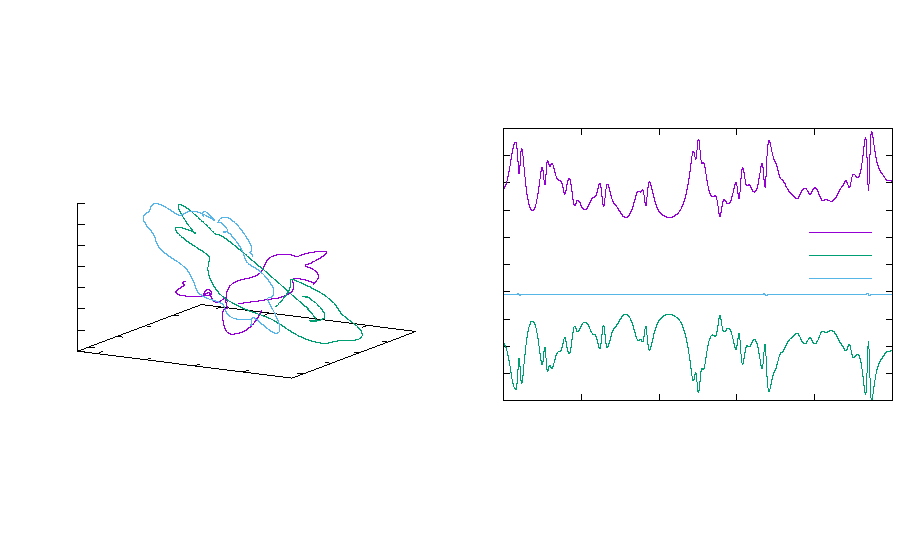
\includegraphics{MDSLP2}}%
    \gplfronttext
  \end{picture}%
\endgroup

	\caption{Trajectories (left) and plot of the kinetic, potential and total energy (right) for a system with $ N = 3 $ particles.}
	\label{fig:MDSLP2}
\end{figure}

\section{Problem 3}
The trajectories and energy plots of systems with $ N = 4 $, $ N = 5 $ and $ N = 6 $ are shown in \cref{fig:MDSLP3N4,fig:MDSLP3N5,fig:MDSLP3N6}.

\begin{figure}[h!]
	\centering
	% GNUPLOT: LaTeX picture with Postscript
\begingroup
  \makeatletter
  \providecommand\color[2][]{%
    \GenericError{(gnuplot) \space\space\space\@spaces}{%
      Package color not loaded in conjunction with
      terminal option `colourtext'%
    }{See the gnuplot documentation for explanation.%
    }{Either use 'blacktext' in gnuplot or load the package
      color.sty in LaTeX.}%
    \renewcommand\color[2][]{}%
  }%
  \providecommand\includegraphics[2][]{%
    \GenericError{(gnuplot) \space\space\space\@spaces}{%
      Package graphicx or graphics not loaded%
    }{See the gnuplot documentation for explanation.%
    }{The gnuplot epslatex terminal needs graphicx.sty or graphics.sty.}%
    \renewcommand\includegraphics[2][]{}%
  }%
  \providecommand\rotatebox[2]{#2}%
  \@ifundefined{ifGPcolor}{%
    \newif\ifGPcolor
    \GPcolorfalse
  }{}%
  \@ifundefined{ifGPblacktext}{%
    \newif\ifGPblacktext
    \GPblacktexttrue
  }{}%
  % define a \g@addto@macro without @ in the name:
  \let\gplgaddtomacro\g@addto@macro
  % define empty templates for all commands taking text:
  \gdef\gplbacktext{}%
  \gdef\gplfronttext{}%
  \makeatother
  \ifGPblacktext
    % no textcolor at all
    \def\colorrgb#1{}%
    \def\colorgray#1{}%
  \else
    % gray or color?
    \ifGPcolor
      \def\colorrgb#1{\color[rgb]{#1}}%
      \def\colorgray#1{\color[gray]{#1}}%
      \expandafter\def\csname LTw\endcsname{\color{white}}%
      \expandafter\def\csname LTb\endcsname{\color{black}}%
      \expandafter\def\csname LTa\endcsname{\color{black}}%
      \expandafter\def\csname LT0\endcsname{\color[rgb]{1,0,0}}%
      \expandafter\def\csname LT1\endcsname{\color[rgb]{0,1,0}}%
      \expandafter\def\csname LT2\endcsname{\color[rgb]{0,0,1}}%
      \expandafter\def\csname LT3\endcsname{\color[rgb]{1,0,1}}%
      \expandafter\def\csname LT4\endcsname{\color[rgb]{0,1,1}}%
      \expandafter\def\csname LT5\endcsname{\color[rgb]{1,1,0}}%
      \expandafter\def\csname LT6\endcsname{\color[rgb]{0,0,0}}%
      \expandafter\def\csname LT7\endcsname{\color[rgb]{1,0.3,0}}%
      \expandafter\def\csname LT8\endcsname{\color[rgb]{0.5,0.5,0.5}}%
    \else
      % gray
      \def\colorrgb#1{\color{black}}%
      \def\colorgray#1{\color[gray]{#1}}%
      \expandafter\def\csname LTw\endcsname{\color{white}}%
      \expandafter\def\csname LTb\endcsname{\color{black}}%
      \expandafter\def\csname LTa\endcsname{\color{black}}%
      \expandafter\def\csname LT0\endcsname{\color{black}}%
      \expandafter\def\csname LT1\endcsname{\color{black}}%
      \expandafter\def\csname LT2\endcsname{\color{black}}%
      \expandafter\def\csname LT3\endcsname{\color{black}}%
      \expandafter\def\csname LT4\endcsname{\color{black}}%
      \expandafter\def\csname LT5\endcsname{\color{black}}%
      \expandafter\def\csname LT6\endcsname{\color{black}}%
      \expandafter\def\csname LT7\endcsname{\color{black}}%
      \expandafter\def\csname LT8\endcsname{\color{black}}%
    \fi
  \fi
    \setlength{\unitlength}{0.0500bp}%
    \ifx\gptboxheight\undefined%
      \newlength{\gptboxheight}%
      \newlength{\gptboxwidth}%
      \newsavebox{\gptboxtext}%
    \fi%
    \setlength{\fboxrule}{0.5pt}%
    \setlength{\fboxsep}{1pt}%
\begin{picture}(8496.00,5040.00)%
    \gplgaddtomacro\gplbacktext{%
      \csname LTb\endcsname%
      \put(475,1695){\makebox(0,0){\strut{}$-2$}}%
      \put(770,1658){\makebox(0,0){\strut{}$-1$}}%
      \put(1064,1621){\makebox(0,0){\strut{}$0$}}%
      \put(1358,1584){\makebox(0,0){\strut{}$1$}}%
      \put(1652,1548){\makebox(0,0){\strut{}$2$}}%
      \put(1947,1511){\makebox(0,0){\strut{}$3$}}%
      \put(2240,1474){\makebox(0,0){\strut{}$4$}}%
      \put(2534,1437){\makebox(0,0){\strut{}$5$}}%
      \put(2771,1478){\makebox(0,0){\strut{}$-1$}}%
      \put(3068,1590){\makebox(0,0){\strut{}$0$}}%
      \put(3366,1702){\makebox(0,0){\strut{}$1$}}%
      \put(3663,1814){\makebox(0,0){\strut{}$2$}}%
      \put(3960,1926){\makebox(0,0){\strut{}$3$}}%
      \put(459,1983){\makebox(0,0)[r]{\strut{}$-2$}}%
      \put(459,2299){\makebox(0,0)[r]{\strut{}$-1$}}%
      \put(459,2615){\makebox(0,0)[r]{\strut{}$0$}}%
      \put(459,2930){\makebox(0,0)[r]{\strut{}$1$}}%
      \put(459,3245){\makebox(0,0)[r]{\strut{}$2$}}%
      \put(-75,2536){\makebox(0,0){\strut{}z}}%
    }%
    \gplgaddtomacro\gplfronttext{%
      \csname LTb\endcsname%
      \put(1318,1365){\makebox(0,0){\strut{}x}}%
      \put(3753,1507){\makebox(0,0){\strut{}y}}%
      \put(-75,2536){\makebox(0,0){\strut{}z}}%
    }%
    \gplgaddtomacro\gplbacktext{%
      \csname LTb\endcsname%
      \put(4540,1587){\makebox(0,0)[r]{\strut{}$-4$}}%
      \put(4540,1927){\makebox(0,0)[r]{\strut{}$-3$}}%
      \put(4540,2266){\makebox(0,0)[r]{\strut{}$-2$}}%
      \put(4540,2606){\makebox(0,0)[r]{\strut{}$-1$}}%
      \put(4540,2946){\makebox(0,0)[r]{\strut{}$0$}}%
      \put(4540,3286){\makebox(0,0)[r]{\strut{}$1$}}%
      \put(4540,3625){\makebox(0,0)[r]{\strut{}$2$}}%
      \put(4540,3965){\makebox(0,0)[r]{\strut{}$3$}}%
      \put(4672,1129){\makebox(0,0){\strut{}$0$}}%
      \put(5420,1129){\makebox(0,0){\strut{}$2$}}%
      \put(6167,1129){\makebox(0,0){\strut{}$4$}}%
      \put(6915,1129){\makebox(0,0){\strut{}$6$}}%
      \put(7662,1129){\makebox(0,0){\strut{}$8$}}%
      \put(8410,1129){\makebox(0,0){\strut{}$10$}}%
    }%
    \gplgaddtomacro\gplfronttext{%
      \csname LTb\endcsname%
      \put(4232,2657){\rotatebox{-270}{\makebox(0,0){\strut{}energy}}}%
      \put(6541,964){\makebox(0,0){\strut{}time t}}%
      \csname LTb\endcsname%
      \put(7480,3023){\makebox(0,0)[r]{\strut{}Kinetic energy}}%
      \csname LTb\endcsname%
      \put(7480,2803){\makebox(0,0)[r]{\strut{}Potential energy}}%
      \csname LTb\endcsname%
      \put(7480,2583){\makebox(0,0)[r]{\strut{}Total energy}}%
    }%
    \gplbacktext
    \put(0,0){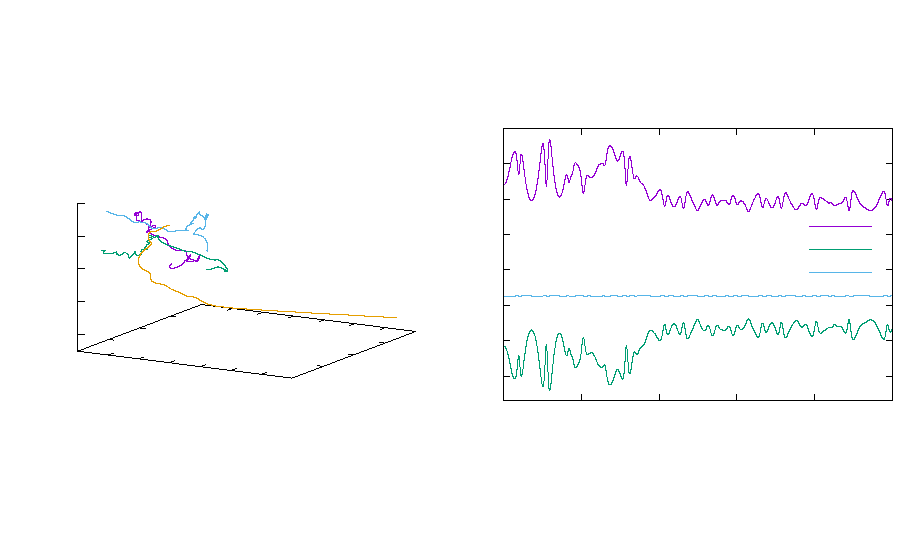
\includegraphics{MDSLP3N4}}%
    \gplfronttext
  \end{picture}%
\endgroup

	\caption{Trajectories (left) and plot of the kinetic, potential and total energy (right) for a system with $ N = 4 $ particles.}
	\label{fig:MDSLP3N4}
\end{figure}

\begin{figure}[h!]
	\centering
	% GNUPLOT: LaTeX picture with Postscript
\begingroup
  \makeatletter
  \providecommand\color[2][]{%
    \GenericError{(gnuplot) \space\space\space\@spaces}{%
      Package color not loaded in conjunction with
      terminal option `colourtext'%
    }{See the gnuplot documentation for explanation.%
    }{Either use 'blacktext' in gnuplot or load the package
      color.sty in LaTeX.}%
    \renewcommand\color[2][]{}%
  }%
  \providecommand\includegraphics[2][]{%
    \GenericError{(gnuplot) \space\space\space\@spaces}{%
      Package graphicx or graphics not loaded%
    }{See the gnuplot documentation for explanation.%
    }{The gnuplot epslatex terminal needs graphicx.sty or graphics.sty.}%
    \renewcommand\includegraphics[2][]{}%
  }%
  \providecommand\rotatebox[2]{#2}%
  \@ifundefined{ifGPcolor}{%
    \newif\ifGPcolor
    \GPcolorfalse
  }{}%
  \@ifundefined{ifGPblacktext}{%
    \newif\ifGPblacktext
    \GPblacktexttrue
  }{}%
  % define a \g@addto@macro without @ in the name:
  \let\gplgaddtomacro\g@addto@macro
  % define empty templates for all commands taking text:
  \gdef\gplbacktext{}%
  \gdef\gplfronttext{}%
  \makeatother
  \ifGPblacktext
    % no textcolor at all
    \def\colorrgb#1{}%
    \def\colorgray#1{}%
  \else
    % gray or color?
    \ifGPcolor
      \def\colorrgb#1{\color[rgb]{#1}}%
      \def\colorgray#1{\color[gray]{#1}}%
      \expandafter\def\csname LTw\endcsname{\color{white}}%
      \expandafter\def\csname LTb\endcsname{\color{black}}%
      \expandafter\def\csname LTa\endcsname{\color{black}}%
      \expandafter\def\csname LT0\endcsname{\color[rgb]{1,0,0}}%
      \expandafter\def\csname LT1\endcsname{\color[rgb]{0,1,0}}%
      \expandafter\def\csname LT2\endcsname{\color[rgb]{0,0,1}}%
      \expandafter\def\csname LT3\endcsname{\color[rgb]{1,0,1}}%
      \expandafter\def\csname LT4\endcsname{\color[rgb]{0,1,1}}%
      \expandafter\def\csname LT5\endcsname{\color[rgb]{1,1,0}}%
      \expandafter\def\csname LT6\endcsname{\color[rgb]{0,0,0}}%
      \expandafter\def\csname LT7\endcsname{\color[rgb]{1,0.3,0}}%
      \expandafter\def\csname LT8\endcsname{\color[rgb]{0.5,0.5,0.5}}%
    \else
      % gray
      \def\colorrgb#1{\color{black}}%
      \def\colorgray#1{\color[gray]{#1}}%
      \expandafter\def\csname LTw\endcsname{\color{white}}%
      \expandafter\def\csname LTb\endcsname{\color{black}}%
      \expandafter\def\csname LTa\endcsname{\color{black}}%
      \expandafter\def\csname LT0\endcsname{\color{black}}%
      \expandafter\def\csname LT1\endcsname{\color{black}}%
      \expandafter\def\csname LT2\endcsname{\color{black}}%
      \expandafter\def\csname LT3\endcsname{\color{black}}%
      \expandafter\def\csname LT4\endcsname{\color{black}}%
      \expandafter\def\csname LT5\endcsname{\color{black}}%
      \expandafter\def\csname LT6\endcsname{\color{black}}%
      \expandafter\def\csname LT7\endcsname{\color{black}}%
      \expandafter\def\csname LT8\endcsname{\color{black}}%
    \fi
  \fi
    \setlength{\unitlength}{0.0500bp}%
    \ifx\gptboxheight\undefined%
      \newlength{\gptboxheight}%
      \newlength{\gptboxwidth}%
      \newsavebox{\gptboxtext}%
    \fi%
    \setlength{\fboxrule}{0.5pt}%
    \setlength{\fboxsep}{1pt}%
\begin{picture}(8496.00,5040.00)%
    \gplgaddtomacro\gplbacktext{%
      \csname LTb\endcsname%
      \put(770,1658){\makebox(0,0){\strut{}$-1$}}%
      \put(1358,1584){\makebox(0,0){\strut{}$0$}}%
      \put(1947,1511){\makebox(0,0){\strut{}$1$}}%
      \put(2534,1437){\makebox(0,0){\strut{}$2$}}%
      \put(2771,1478){\makebox(0,0){\strut{}$-1$}}%
      \put(3167,1627){\makebox(0,0){\strut{}$0$}}%
      \put(3564,1777){\makebox(0,0){\strut{}$1$}}%
      \put(3960,1926){\makebox(0,0){\strut{}$2$}}%
      \put(459,1825){\makebox(0,0)[r]{\strut{}$-1$}}%
      \put(459,2231){\makebox(0,0)[r]{\strut{}$0$}}%
      \put(459,2636){\makebox(0,0)[r]{\strut{}$1$}}%
      \put(459,3042){\makebox(0,0)[r]{\strut{}$2$}}%
      \put(-75,2536){\makebox(0,0){\strut{}z}}%
    }%
    \gplgaddtomacro\gplfronttext{%
      \csname LTb\endcsname%
      \put(1318,1365){\makebox(0,0){\strut{}x}}%
      \put(3753,1507){\makebox(0,0){\strut{}y}}%
      \put(-75,2536){\makebox(0,0){\strut{}z}}%
    }%
    \gplgaddtomacro\gplbacktext{%
      \csname LTb\endcsname%
      \put(4540,1587){\makebox(0,0)[r]{\strut{}$-6$}}%
      \put(4540,2062){\makebox(0,0)[r]{\strut{}$-4$}}%
      \put(4540,2538){\makebox(0,0)[r]{\strut{}$-2$}}%
      \put(4540,3014){\makebox(0,0)[r]{\strut{}$0$}}%
      \put(4540,3489){\makebox(0,0)[r]{\strut{}$2$}}%
      \put(4540,3965){\makebox(0,0)[r]{\strut{}$4$}}%
      \put(4672,1129){\makebox(0,0){\strut{}$0$}}%
      \put(5420,1129){\makebox(0,0){\strut{}$2$}}%
      \put(6167,1129){\makebox(0,0){\strut{}$4$}}%
      \put(6915,1129){\makebox(0,0){\strut{}$6$}}%
      \put(7662,1129){\makebox(0,0){\strut{}$8$}}%
      \put(8410,1129){\makebox(0,0){\strut{}$10$}}%
    }%
    \gplgaddtomacro\gplfronttext{%
      \csname LTb\endcsname%
      \put(4232,2657){\rotatebox{-270}{\makebox(0,0){\strut{}energy}}}%
      \put(6541,964){\makebox(0,0){\strut{}time t}}%
      \csname LTb\endcsname%
      \put(7480,3035){\makebox(0,0)[r]{\strut{}Kinetic energy}}%
      \csname LTb\endcsname%
      \put(7480,2815){\makebox(0,0)[r]{\strut{}Potential energy}}%
      \csname LTb\endcsname%
      \put(7480,2595){\makebox(0,0)[r]{\strut{}Total energy}}%
    }%
    \gplbacktext
    \put(0,0){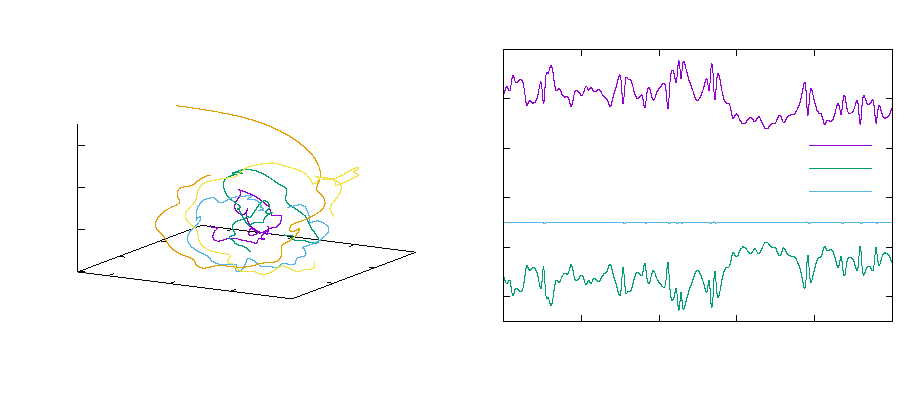
\includegraphics{MDSLP3N5}}%
    \gplfronttext
  \end{picture}%
\endgroup

	\caption{Trajectories (left) and plot of the kinetic, potential and total energy (right) for a system with $ N = 5 $ particles.}
	\label{fig:MDSLP3N5}
\end{figure}

\begin{figure}[h!]
	\centering
	% GNUPLOT: LaTeX picture with Postscript
\begingroup
  \makeatletter
  \providecommand\color[2][]{%
    \GenericError{(gnuplot) \space\space\space\@spaces}{%
      Package color not loaded in conjunction with
      terminal option `colourtext'%
    }{See the gnuplot documentation for explanation.%
    }{Either use 'blacktext' in gnuplot or load the package
      color.sty in LaTeX.}%
    \renewcommand\color[2][]{}%
  }%
  \providecommand\includegraphics[2][]{%
    \GenericError{(gnuplot) \space\space\space\@spaces}{%
      Package graphicx or graphics not loaded%
    }{See the gnuplot documentation for explanation.%
    }{The gnuplot epslatex terminal needs graphicx.sty or graphics.sty.}%
    \renewcommand\includegraphics[2][]{}%
  }%
  \providecommand\rotatebox[2]{#2}%
  \@ifundefined{ifGPcolor}{%
    \newif\ifGPcolor
    \GPcolorfalse
  }{}%
  \@ifundefined{ifGPblacktext}{%
    \newif\ifGPblacktext
    \GPblacktexttrue
  }{}%
  % define a \g@addto@macro without @ in the name:
  \let\gplgaddtomacro\g@addto@macro
  % define empty templates for all commands taking text:
  \gdef\gplbacktext{}%
  \gdef\gplfronttext{}%
  \makeatother
  \ifGPblacktext
    % no textcolor at all
    \def\colorrgb#1{}%
    \def\colorgray#1{}%
  \else
    % gray or color?
    \ifGPcolor
      \def\colorrgb#1{\color[rgb]{#1}}%
      \def\colorgray#1{\color[gray]{#1}}%
      \expandafter\def\csname LTw\endcsname{\color{white}}%
      \expandafter\def\csname LTb\endcsname{\color{black}}%
      \expandafter\def\csname LTa\endcsname{\color{black}}%
      \expandafter\def\csname LT0\endcsname{\color[rgb]{1,0,0}}%
      \expandafter\def\csname LT1\endcsname{\color[rgb]{0,1,0}}%
      \expandafter\def\csname LT2\endcsname{\color[rgb]{0,0,1}}%
      \expandafter\def\csname LT3\endcsname{\color[rgb]{1,0,1}}%
      \expandafter\def\csname LT4\endcsname{\color[rgb]{0,1,1}}%
      \expandafter\def\csname LT5\endcsname{\color[rgb]{1,1,0}}%
      \expandafter\def\csname LT6\endcsname{\color[rgb]{0,0,0}}%
      \expandafter\def\csname LT7\endcsname{\color[rgb]{1,0.3,0}}%
      \expandafter\def\csname LT8\endcsname{\color[rgb]{0.5,0.5,0.5}}%
    \else
      % gray
      \def\colorrgb#1{\color{black}}%
      \def\colorgray#1{\color[gray]{#1}}%
      \expandafter\def\csname LTw\endcsname{\color{white}}%
      \expandafter\def\csname LTb\endcsname{\color{black}}%
      \expandafter\def\csname LTa\endcsname{\color{black}}%
      \expandafter\def\csname LT0\endcsname{\color{black}}%
      \expandafter\def\csname LT1\endcsname{\color{black}}%
      \expandafter\def\csname LT2\endcsname{\color{black}}%
      \expandafter\def\csname LT3\endcsname{\color{black}}%
      \expandafter\def\csname LT4\endcsname{\color{black}}%
      \expandafter\def\csname LT5\endcsname{\color{black}}%
      \expandafter\def\csname LT6\endcsname{\color{black}}%
      \expandafter\def\csname LT7\endcsname{\color{black}}%
      \expandafter\def\csname LT8\endcsname{\color{black}}%
    \fi
  \fi
    \setlength{\unitlength}{0.0500bp}%
    \ifx\gptboxheight\undefined%
      \newlength{\gptboxheight}%
      \newlength{\gptboxwidth}%
      \newsavebox{\gptboxtext}%
    \fi%
    \setlength{\fboxrule}{0.5pt}%
    \setlength{\fboxsep}{1pt}%
\begin{picture}(8496.00,3528.00)%
    \gplgaddtomacro\gplbacktext{%
      \csname LTb\endcsname%
      \put(819,896){\makebox(0,0){\strut{}$0$}}%
      \put(1505,810){\makebox(0,0){\strut{}$1$}}%
      \put(2192,724){\makebox(0,0){\strut{}$2$}}%
      \put(2771,722){\makebox(0,0){\strut{}$-1$}}%
      \put(3167,871){\makebox(0,0){\strut{}$0$}}%
      \put(3564,1021){\makebox(0,0){\strut{}$1$}}%
      \put(3960,1170){\makebox(0,0){\strut{}$2$}}%
      \put(459,1069){\makebox(0,0)[r]{\strut{}$-1$}}%
      \put(459,1475){\makebox(0,0)[r]{\strut{}$0$}}%
      \put(459,1880){\makebox(0,0)[r]{\strut{}$1$}}%
      \put(459,2286){\makebox(0,0)[r]{\strut{}$2$}}%
      \put(-75,1780){\makebox(0,0){\strut{}z}}%
    }%
    \gplgaddtomacro\gplfronttext{%
      \csname LTb\endcsname%
      \put(1318,609){\makebox(0,0){\strut{}x}}%
      \put(3753,751){\makebox(0,0){\strut{}y}}%
      \put(-75,1780){\makebox(0,0){\strut{}z}}%
    }%
    \gplgaddtomacro\gplbacktext{%
      \csname LTb\endcsname%
      \put(4540,747){\makebox(0,0)[r]{\strut{}$-10$}}%
      \put(4540,1055){\makebox(0,0)[r]{\strut{}$-8$}}%
      \put(4540,1362){\makebox(0,0)[r]{\strut{}$-6$}}%
      \put(4540,1670){\makebox(0,0)[r]{\strut{}$-4$}}%
      \put(4540,1978){\makebox(0,0)[r]{\strut{}$-2$}}%
      \put(4540,2286){\makebox(0,0)[r]{\strut{}$0$}}%
      \put(4540,2593){\makebox(0,0)[r]{\strut{}$2$}}%
      \put(4540,2901){\makebox(0,0)[r]{\strut{}$4$}}%
      \put(4540,3209){\makebox(0,0)[r]{\strut{}$6$}}%
      \put(4672,373){\makebox(0,0){\strut{}$0$}}%
      \put(5420,373){\makebox(0,0){\strut{}$2$}}%
      \put(6167,373){\makebox(0,0){\strut{}$4$}}%
      \put(6915,373){\makebox(0,0){\strut{}$6$}}%
      \put(7662,373){\makebox(0,0){\strut{}$8$}}%
      \put(8410,373){\makebox(0,0){\strut{}$10$}}%
    }%
    \gplgaddtomacro\gplfronttext{%
      \csname LTb\endcsname%
      \put(4100,1901){\rotatebox{-270}{\makebox(0,0){\strut{}energy}}}%
      \put(6541,208){\makebox(0,0){\strut{}time t}}%
      \csname LTb\endcsname%
      \put(7480,2260){\makebox(0,0)[r]{\strut{}Kinetic energy}}%
      \csname LTb\endcsname%
      \put(7480,2040){\makebox(0,0)[r]{\strut{}Potential energy}}%
      \csname LTb\endcsname%
      \put(7480,1820){\makebox(0,0)[r]{\strut{}Total energy}}%
    }%
    \gplbacktext
    \put(0,0){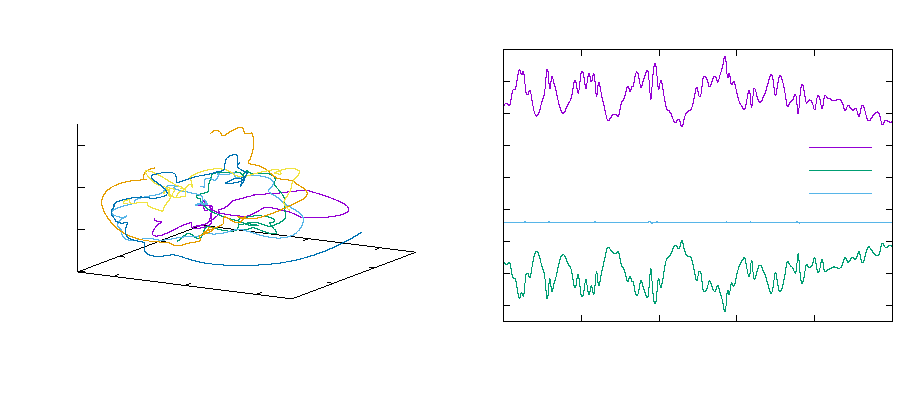
\includegraphics{MDSLP3N6}}%
    \gplfronttext
  \end{picture}%
\endgroup

	\caption{Trajectories (left) and plot of the kinetic, potential and total energy (right) for a system with $ N = 6 $ particles.}
	\label{fig:MDSLP3N6}
\end{figure}

\section{Problem 4}
\todo{Problem 4 maken}

\section{Problem 5}
\todo{Problem 5 maken}

\section{Problem 6}
\todo{Problem 6 maken}

\section{Problem 7}
\todo{Problem 7 maken}

\section{Problem 8}
\todo{Problem 8 maken}

\section{Problem 9}
\todo{Problem 9 maken}

\section{Master exercise}
\todo[inline]{choose 1 of the master exercises}

\insertbibliography
%\begin{appendices}
%% appendices hier
%
%
%\end{appendices}


\end{document}